\chapter{Event- and LiDAR-Based Depth Estimation using an Attention-Based Network}\label{sec:delta}

As noted in the conclusion of \cref{sec:aled}, our \acrshort{aled} network has two main issues:
\begin{enumerate*}[label=\textbf{(\arabic*)}]
  \item it shows large errors for close distances, something we want to avoid for robotic applications, and
  \item it can only predict dense depth maps, from which we can associate depths to each event, but at the cost of some accuracy. 
\end{enumerate*}
In this chapter, we aim at exploring these two issues and seeing how they could be solved using an attention-based network, which should allow for a better understanding of interactions between event and LiDAR data, and could theoretically allow for a sparse depth estimation without needing any dense frame-based representation.

The presented method and the associated results of this chapter were submitted as part of the ECCV 2024 conference. Since ECCV is a double-blind conference, a public project page is not yet available at the time of writing of this thesis, but a private playlist of videos showcasing some results is available at \url{https://www.youtube.com/playlist?list=PLLL0eWAd6OXBKmvfUNCR21iq2C4Ck8-B4}.

\section{Introduction}
Attention-based networks like the Transformer~\cite{Vaswani2017AttentionIA} are particularly powerful when it comes to representing interactions between elements of a sequence, like words in a sentence. While originally intended for \acrfull{nlp}, they have since become the standard architecture in numerous domains, including computer vision, and have shown impressive capabilities for multimodal data fusion~\cite{Prakash2021MultiModalFT,Chitta2022TransFuserIW}.

Therefore, in this chapter, we still aim at fusing sparse LiDAR and event data available at different rates, but doing it with an attention-based network. As will be described in the following sections, while our initial goal was to accomplish this fusion directly on sparse inputs and outputs, several theoretical and technical limitations were met. Therefore, we returned to denser representations, and propose here a novel attention-based network which we call \acrshort{delta}, able to combine information from low-rate projected LiDAR point clouds with higher-rate small temporal windows of events, in order to derive accurate dense depth maps.

Thanks to its attention- and recurrence-based design, we show that this network is able to extract the most relevant spatial and temporal features within and in-between the event and LiDAR data. The introduction of a propagation memory for fusion at the highest input rate and of a central memory acting as a main recurrence both allow us to outperform the state of the art, and are critical contributions as shown through an ablation study.

As for previous chapters, an extensive evaluation of \acrshort{delta} is conducted on multiple automotive datasets, where LiDAR and event sensors are most commonly used together. We show here that \acrshort{delta} is able to offer a clear improvement from \acrshort{aled} and the rest of the state of the art, in particular for close objects (which was the main limitation of \acrshort{aled}), where the average error is reduced up to four times.

This chapter is structured as follows. We first give an introduction to how the Transformer model and especially its attention mechanism work in \cref{sec:delta:intro_transf_att}. We then give an overview of the state of the art in \cref{sec:delta:sota}. We describe our attempts at estimating directly sparse depths and the issues we faced in \cref{sec:delta:sparse_network}, and our final dense solution in \cref{sec:delta:method}. We finally conduct our evaluation in \cref{sec:delta:eval}, before drawing some conclusions in \cref{sec:delta:conclusion}.


\section{An Introduction to the Transformer and Attention}\label{sec:delta:intro_transf_att}
Before going into the details of the work conducted in this chapter, we must take some time to explain how the Transformer architecture works, and especially its attention module.

\subsection{Overview of the Transformer Architecture}
The Transformer~\cite{Vaswani2017AttentionIA} is a novel neural network model proposed in 2017, originally intended for \acrfull{nlp}. The objective of this model was to answer the limitations met by former recurrence-based networks (such as \acrshortpl{lstm}): a tendency to forget context for long input sequences, and slow training and inference times due to their one-by-one processing of words. To solve these issues, the Transformer is able to treat the full input sequence in parallel at once, i.e., without splitting it into word-by-word inputs, and by explicitly modeling the relations between each word.

\begin{figure}
  \centering

  % Defining the colors that will be used
  \definecolor{color_em}{RGB}{255,255,255}
  \definecolor{color_sa}{RGB}{102,204,238}
  \definecolor{color_ca}{RGB}{68,119,170}
  \definecolor{color_ff}{RGB}{204,187,68}
  \definecolor{color_ls}{RGB}{187,187,187}

  \begin{subfigure}{0.7\linewidth}
    \centering
    \resizebox{\linewidth}{!}{
      \begin{tikzpicture}[every node/.style={outer sep=0.001}]
        % Changing the font
        \fontfamily{cmss}\selectfont

        % Input encoding
        \node (I) at (0,0) {Inputs};

        \node[draw, fill=color_em, rounded corners, minimum width=2.75cm, above=1cm of I, align=center] (Ie) {Input\\Embedding};

        \node[draw, circle, inner sep=0.001, minimum width=0.5cm, above=1cm of Ie] (Ip) {+};

        \node[draw, circle, minimum width=1cm, minimum height=1cm, left=1cm of Ip] (IPE) {};
        \draw[thick] ($(IPE)+(-0.5cm,0)$) sin ($(IPE)+(-0.25cm,0.3cm)$) cos (IPE) sin ($(IPE)+(0.25cm,-0.3cm)$) cos ($(IPE)+(0.5cm,0)$);

        \node[left=0.5cm of IPE, align=right] (IPEl) {Positional\\Encoding};

        % Self-attention encoders
        \node[draw, fill=color_sa, rounded corners, minimum width=2.75cm, above=1cm of Ip, align=center] (ISA) {Self-\\Attention};
        \node[draw, fill=color_ff, rounded corners, minimum width=2.75cm, above=1cm of ISA, align=center] (IFF) {Feed-Forward\\Block};

        \node[label={left:N\texttimes{}},draw,thick,dotted,fit=(ISA)(IFF)] {};

        % Masked self-attention decoders
        \node[draw, fill=color_sa, rounded corners, minimum width=2.75cm, right=2cm of ISA, align=center] (OSA) {Self-\\Attention};
        \node[draw, fill=color_ca, rounded corners, minimum width=2.75cm, above=1cm of OSA, align=center] (OCA) {Cross-\\Attention};
        \node[draw, fill=color_ff, rounded corners, minimum width=2.75cm, above=1cm of OCA, align=center] (OFF) {Feed-Forward\\Block};

        \node[label={right:\texttimes{}N},draw,thick,dotted,fit=(OSA)(OCA)(OFF)] {};

        % Output input encoding
        \node[draw, circle, inner sep=0.001, minimum width=0.5cm, below=1cm of OSA] (Op) {+};

        \node[draw, circle, minimum width=1cm, minimum height=1cm, right=1cm of Op] (OPE) {};
        \draw[thick] ($(OPE)+(-0.5cm,0)$) sin ($(OPE)+(-0.25cm,0.3cm)$) cos (OPE) sin ($(OPE)+(0.25cm,-0.3cm)$) cos ($(OPE)+(0.5cm,0)$);

        \node[draw, fill=color_em, rounded corners, minimum width=2.75cm, below=1cm of Op, align=center] (Oe) {Output\\Embedding};

        \node[right=0.5cm of OPE, align=left] (OPEl) {Positional\\Encoding};

        \node[below=1cm of Oe, align=center] (OI) {Previous\\Outputs};

        % Output decoding
        \node[draw, fill=color_ls, rounded corners, minimum width=2.75cm, above=1cm of OFF, align=center] (LPS) {Linear +\\Softmax};

        \node[above=1cm of LPS, align=center] (O) {Output\\Probabilities};

        % Paths
        \draw[->,>=latex, line width=0.3mm] (I) -- (Ie);
        \draw[->,>=latex, line width=0.3mm] (Ie) -- (Ip);
        \draw[->,>=latex, line width=0.3mm] (IPE) -- (Ip);
        \draw[->,>=latex, line width=0.3mm] (Ip) -- (ISA);
        \draw[->,>=latex, line width=0.3mm] (ISA) -- (IFF);

        \draw[->,>=latex, line width=0.3mm] (OI) -- (Oe);
        \draw[->,>=latex, line width=0.3mm] (Oe) -- (Op);
        \draw[->,>=latex, line width=0.3mm] (OPE) -- (Op);
        \draw[->,>=latex, line width=0.3mm] (Op) -- (OSA);
        \draw[->,>=latex, line width=0.3mm] (OSA) -- node [left=0.1cm, pos=0.7, inner sep=0.001] {\color{color_ca} \textbf{Q}} (OCA);
        \draw[->,>=latex, line width=0.3mm] (OCA) -- (OFF);
        \draw[->,>=latex, line width=0.3mm] (OFF) -- (LPS);
        \draw[->,>=latex, line width=0.3mm] (LPS) -- (O);

        \draw[->,>=latex, line width=0.3mm] (IFF) -- ($(IFF.north)+(0,0.5cm)$) -- ($(IFF.north)+(1.875cm,0.5cm)$) -- ($(OCA.west)+(-1.5cm,0)$) -- node [above=0.05cm, pos=0.6, inner sep=0.001] {\color{color_ca} \textbf{K/V}} (OCA);
      \end{tikzpicture}
    }
    \subcaption{Simplified view of the Transformer architecture.}\label{fig:delta:transformer:overview}
  \end{subfigure}
  \hfill
  \vline{}
  \hfill
  \begin{subfigure}{0.25\linewidth}
    \centering
    \resizebox{0.65\linewidth}{!}{
      \begin{tikzpicture}[every node/.style={outer sep=0.001}]
        % Changing the font
        \fontfamily{cmss}\selectfont

        \node[draw, fill=color_sa, rounded corners, minimum width=2.75cm, align=center] (MHA) at (0,0) {Multi-Head\\Attention};
        \node[draw, fill=color_sa, rounded corners, minimum width=2.75cm, above=0.5cm of MHA, align=center] (AN) {Add \& Norm};

        \draw[->,>=latex, line width=0.3mm] ($(MHA.south)-(0,0.65cm)$) -- ($(MHA.south)-(1cm,0.65cm)$) -- node [right=0.05cm, pos=0.4, inner sep=0.001] {\color{color_ca} \textbf{Q}} ($(MHA.south)-(1cm,0)$);
        \draw[->,>=latex, line width=0.3mm] ($(MHA.south)-(0,1.5cm)$) -- ($(MHA.south)-(0,0.65cm)$) -- node [right=0.05cm, pos=0.4, inner sep=0.001] {\color{color_ca} \textbf{K}} (MHA);
        \draw[->,>=latex, line width=0.3mm] ($(MHA.south)-(0,0.65cm)$) -- ($(MHA.south)+(1cm,-0.65cm)$) -- node [right=0.05cm, pos=0.4, inner sep=0.001] {\color{color_ca} \textbf{V}} ($(MHA.south)+(1cm,0)$);
        \draw[->,>=latex, line width=0.3mm] ($(MHA.south)-(0,1cm)$) -- ($(MHA.south)-(1.875cm,1cm)$) -- ($(AN.west)-(0.5cm,0)$) -- (AN);
        \draw[->,>=latex, line width=0.3mm] (MHA) -- (AN);
        \draw[->,>=latex, line width=0.3mm] (AN) -- ($(AN.north)+(0,0.5cm)$);
      \end{tikzpicture}
    }
    \subcaption{Detailed Self-Attention block}\label{fig:delta:transformer:sa}

    \resizebox{0.65\linewidth}{!}{
      \begin{tikzpicture}[every node/.style={outer sep=0.001}]
        % Changing the font
        \fontfamily{cmss}\selectfont

        \node[draw, fill=color_ca, rounded corners, minimum width=2.75cm, align=center] (MHA) at (0,0) {Multi-Head\\Attention};
        \node[draw, fill=color_ca, rounded corners, minimum width=2.75cm, above=0.5cm of MHA, align=center] (AN) {Add \& Norm};

        \draw[->,>=latex, line width=0.3mm] ($(MHA.south)-(1cm,1.5cm)$) -- ($(MHA.south)-(1cm,0.65cm)$) -- node [right=0.05cm, pos=0.4, inner sep=0.001] {\color{color_ca} \textbf{Q}} ($(MHA.south)-(1cm,0)$);
        \draw[->,>=latex, line width=0.3mm] ($(MHA.south)+(0.5cm,-1.5cm)$) -- ($(MHA.south)+(0.5cm,-0.65cm)$) -- ($(MHA.south)+(0,-0.65cm)$) -- node [right=0.05cm, pos=0.4, inner sep=0.001] {\color{color_ca} \textbf{K}} (MHA);
        \draw[->,>=latex, line width=0.3mm] ($(MHA.south)+(0.5cm,-0.65cm)$) -- ($(MHA.south)+(1cm,-0.65cm)$) -- node [right=0.05cm, pos=0.4, inner sep=0.001] {\color{color_ca} \textbf{V}} ($(MHA.south)+(1cm,0)$);
        \draw[->,>=latex, line width=0.3mm] ($(MHA.south)-(1cm,1cm)$) -- ($(MHA.south)-(1.875cm,1cm)$) -- ($(AN.west)-(0.5cm,0)$) -- (AN);
        \draw[->,>=latex, line width=0.3mm] (MHA) -- (AN);
        \draw[->,>=latex, line width=0.3mm] (AN) -- ($(AN.north)+(0,0.5cm)$);
      \end{tikzpicture}
    }
    \subcaption{Detailed Cross-Attention block}\label{fig:delta:transformer:ca}

    \resizebox{0.65\linewidth}{!}{
      \begin{tikzpicture}[every node/.style={outer sep=0.001}]
        % Changing the font
        \fontfamily{cmss}\selectfont

        \node[draw, fill=color_ff, rounded corners, minimum width=2.75cm, align=center] (FFL) at (0,0) {Feed-Forward\\Layer};
        \node[draw, fill=color_ff, rounded corners, minimum width=2.75cm, above=0.5cm of FFL, align=center] (AN) {Add \& Norm};

        \draw[->,>=latex, line width=0.3mm] ($(FFL.south)-(0,1cm)$) -- (FFL);
        \draw[->,>=latex, line width=0.3mm] ($(FFL.south)-(0,0.5cm)$) -- ($(FFL.south)-(1.875cm,0.5cm)$) -- ($(AN.west)-(0.5cm,0)$) -- (AN);
        \draw[->,>=latex, line width=0.3mm] (FFL) -- (AN);
        \draw[->,>=latex, line width=0.3mm] (AN) -- ($(AN.north)+(0,0.5cm)$);
      \end{tikzpicture}
    }
    \subcaption{Detailed Feed-Forward block}\label{fig:delta:transformer:ff}
  \end{subfigure}
  \caption{Overview of the Transformer architecture. Illustration inspired by~\cite{Vaswani2017AttentionIA}.}\label{fig:delta:transformer}
\end{figure}

To do so, as illustrated in \cref{fig:delta:transformer:overview}, each input word is converted into a token, i.e., a fixed-size vector representation of this word. As the Transformer is an order independent architecture, a positional encoding is added to each token, representing its position in the input sequence. This list of tokens is then given to an attention-based encoder-decoder which we will describe in the next paragraphs. The decoder also takes as input the previously predicted output tokens. A final linear+softmax layer is used to give probabilities over the full dictionary of words, with the word with the best probability being added as the next word to the previously predicted words. This process is repeated until the network predicts a special \acrfull{eos} token.

Regarding the encoder itself, it is composed of \(N\) successive blocks, each composed of a self-attention block (illustrated in \cref{fig:delta:transformer:sa}, tasked with representing the relations within the tokens, as will be explained in \cref{sec:delta:intro_transf_att:full_att}) and a feed-forward block (illustrated in \cref{fig:delta:transformer:ff}, tasked with refining the output of the self-attention block).

As for the decoder, it is also composed of \(N\) successive blocks, each composed of a self-attention block, a cross-attention block (illustrated in \cref{fig:delta:transformer:ca}, tasked with representing the relations between the previously predicted tokens and the encoded input tokens, as will also be explained in \cref{sec:delta:intro_transf_att:full_att}), and a feed-forward block.

In the following parts of this chapter, for simplicity of notation and of representation, we will note ``\textit{self-attention module}'' the block composed of a self-attention block (\smbluesquare{}) followed by a feed-forward block (\smyellowsquare{}), and ``\textit{cross-attention module}'' the block composed of a cross-attention block (\smdarkbluesquare{}) followed by a feed-forward block (\smyellowsquare{}).

\subsection{Full Attention}\label{sec:delta:intro_transf_att:full_att}
As noted before, the core element of the Transformer is its concept of attention, for representing explicitly relations within elements of a single sequence, or in-between elements of two sequences. This notion is particularly important typically (but not only) for \acrshort{nlp}: in a simple sentence like ``The cat could not eat its meal because \textit{it} was ill.'', understanding that the word ``\textit{it}'' refers to the cat rather than to the meal is non-trivial for a machine; being able to represent this relation explicitly is therefore important for a good learning.

While the concept of attention is not new (we can cite here the articles of Nadaraya and of Watson~\cite{Nadaraya1964OnER,Watson1964SmoothRA} both published in 1964, or the more recent article of Bahdanau \textit{et al.}~\cite{Bahdanau2014NeuralMT}), the Transformer was the first to propose a fully parallelizable formulation of attention, particularly suited for learning on large sequences. In their formulation, they consider three input matrices: a matrix of queries \(Q\) of shape \((N_Q, D)\), a matrix of keys \(K\) of shape \((N_{KV}, D)\), and a matrix of values \(V\) of shape \((N_{KV}, D)\), where \(N_Q\) and \(N_{KV}\) are respectively the number of vectors of queries and keys/values, and \(D\) is the dimensionality (i.e., the length) of the vectors.

They first compute a matrix of attention scores \(S\) by putting in relation the queries and the keys, i.e., by determining how the queries ``match'' the keys:
\begin{equation}
  S = \text{softmax}\left(\frac{QK^T}{\sqrt{D}}\right) \label{eq:delta:att_score}
\end{equation}
where \(S\) is of shape \((N_Q, N_{KV})\). By using the softmax, each of the \(N_Q\) rows contains a score for each of the keys, summing to 1. This matrix of attention scores is finally applied on the matrix of values, to obtain the final matrix of values after receiving attention \(A\):
\begin{equation}
  A = SV \label{eq:delta:att_values}
\end{equation}
where \(A\) is of the same shape as the queries, i.e., \((N_Q, D)\).

In practice, in case of self-attention, the three matrices \(Q\), \(K\), and \(V\) are obtained by multiplying the single input matrix \(I\) by matrices of learned weights \(W_Q\), \(W_K\), and \(W_V\):
\begin{align}
  Q &= I W_Q \nonumber\\
  K &= I W_K \\
  V &= I W_V \nonumber
\end{align}
In case of cross-attention, two input matrices are used, \(I_1\) and \(I_2\), and the \(Q\), \(K\), and \(V\) matrices are computed as:
\begin{align}
  Q &= I_1 W_Q \nonumber\\
  K &= I_2 W_K \\
  V &= I_2 W_V \nonumber
\end{align}
Therefore, self-attention is just a special case of cross-attention, where \(I_1 = I_2\).

\subsection{Linearized Attention}\label{sec:delta:intro_transf_att:lin_att}
As shown in \cref{eq:delta:att_score}, the matrix of attention scores \(S\) is of shape \((N_Q, N_{KV})\) (due to the multiplication of \(Q\) and \(K^T\)). Therefore, and since \(N_Q \gg D\) and \(N_{KV} \gg D\), the space complexity of the attention process is of
\begin{equation}
  \mathcal{O}(N_Q\times{}N_{KV}+N_Q\times{}D) \simeq \mathcal{O}(N^2) \label{eq:delta:full_att_complexity}
\end{equation}
i.e., it grows quadratically. In case of long input sequences, this memory requirement can quickly become a limitation. Therefore, several authors have proposed linearized versions of the attention process. We describe here the two formulations that we tested as part of our work, that both rely on the same core idea: reducing the space complexity by carrying out the multiplication of \(K^T\) and \(V\) first.

As shown by Katharopoulos \textit{et al.}~\cite{Katharopoulos2020TransformersAR}, \cref{eq:delta:att_score,eq:delta:att_values} can be generalized and rewritten as
\begin{equation}
  \left(\phi(Q) \phi(K)^T\right) V = \phi(Q) \left(\phi(K)^T V\right)
\end{equation}
where \(\phi(\cdot)\) is a feature map. Using the second formulation, the multiplication between \(K^T\) and \(V\) is applied first, resulting in a space complexity for the attention process of
\begin{equation}
  \mathcal{O}(D\times{}D+N_Q\times{}D) \simeq \mathcal{O}(N) \label{eq:delta:lin_att_complexity}
\end{equation}
i.e., a memory usage which grows linearly.

In their article, Katharopoulos \textit{et al.}~\cite{Katharopoulos2020TransformersAR} use the exponential linear unit function~\cite{Clevert2016FastAA} \(\text{elu}(\cdot)\) as their feature map:
\begin{equation}
  \phi(x) = \text{elu}(x) + 1
\end{equation}
Comparatively, Kamal \textit{et al.}~\cite{Kamal2023AssociativeMA} use the softmax activation function as their feature map:
\begin{equation}
  \phi(x) = \text{softmax}(x)
\end{equation}

However, as investigated by~\cite{Narang2021DoTM,Tay2022ScalingLV}, linear attention limits the ability of networks to train efficiently, reducing their maximum theoretical accuracy.

\section{Related Work}\label{sec:delta:sota}

\subsection{Transformers for Event-Based Data}
The Transformer~\cite{Vaswani2017AttentionIA} has become the state-of-the-art architecture in numerous domains. Its attention mechanism models explicitly the relations between relevant elements in a sequence, making it able to understand structures. For computer vision, the arrival of the Vision Transformer~\cite{Dosovitskiy2020AnII} has been a notable landmark, by outperforming more traditional convolution-based networks. As such, researchers have started investigating how the Transformer architecture could be adapted to event-based cameras. Two philosophies have emerged over the years.
\begin{enumerate*}[label=\textbf{(\arabic*)}]
  \item Some authors use directly the raw stream of events (without any pre-processing) as the input sequence to their network, and use the Transformer architecture to process it. This approach is particularly complex, as each event contains little information, making the modeling of their relations difficult for the Transformer. To contain enough context, sequences of events should also be of consequent size, whereas the Transformer was designed for smaller sequences. As such, this method has only been applied to the task of classification~\cite{Kamal2023AssociativeMA,Li2022EventT}, where the event data can be highly compressed by the network, as the final representation is only a small vector.
  \item To circumvent these issues, most authors instead accumulate events in a frame-like representation, and process it using a mixture of convolutional layers and of Transformer blocks. Investigated tasks include object detection~\cite{Gehrig2022RecurrentVT}, classification~\cite{Sabater2022EventTA+,Wang2022ExploitingSS,Sabater2022EventTA}, depth estimation~\cite{Sabater2022EventTA+}, optical flow~\cite{Tian2022EventTF}, and video reconstruction~\cite{Weng2021EventbasedVR}.
\end{enumerate*}

\subsection{Fusion of Events and LiDAR}
As seen throughout \cref{sec:aled}, to this day, most works using both the LiDAR and event-based modalities address the problem of extrinsic calibration~\cite{Song2018CalibrationOE,Ta2022L2ELT,Jiao2023LCECalibAL}, or use them as part of the construction of a dataset~\cite{Zhu2018TheMS,Gehrig2021DSECAS,Chaney2023M3EDMM}. Recently, authors have started investigating the issues of enhancing point clouds with event-based data~\cite{Li2021Enhancing3L}, of estimating dense depth maps from event and LiDAR data~\cite{Cui2022DenseDE}, and of human tracking in adversarial lighting conditions~\cite{Saucedo2023EventCA}.

\subsection{Depth Estimation using Events}
The idea of estimating sparse or dense depth maps from events has been actively explored over the past decade. Three main approaches can be distinguished.
\begin{enumerate*}[label=\textbf{(\arabic*)}]
  \item Some authors estimate depths in a monocular fashion, using only events from a single event camera~\cite{Zhu2019UnsupervisedEL,Ranon2021StereoSpikeDL,Kim2016RealTime3R,HidalgoCarrio2020LearningMD,Chiavazza2023LowlatencyMD,Nunes2023TimetocontactMB}, or using events and frames~\cite{Gehrig2021CombiningEA,Sabater2022EventTA+} from a DAVIS camera~\cite{Brandli2014A2}. These approaches are particularly challenging, as they lack any three dimensional information, and tend to result in overall lower performances.
  \item Some authors have tried to estimate depth in a stereo fashion, by using a pair of event cameras~\cite{Ranon2021StereoSpikeDL,Schraml2010DynamicSV,Schraml2016AnES,Nam2022StereoDF,Cho2023LearningAD,Ghosh2022MultiEventCameraDE}, with~\cite{Cho2023LearningAD} and~\cite{Ranon2021StereoSpikeDL} achieving notably good results.
  \item Finally, some authors prefer to use directly a depth sensor, and use the stream of event as a mean to densify and/or to temporally upsample the depth data. This depth sensor can either be an RGB-D camera~\cite{Weikersdorfer2014Eventbased3S} or a LiDAR~\cite{Li2021Enhancing3L,Cui2022DenseDE,Brebion2023LearningTE}, with our work described in the previous chapter~\cite{Brebion2023LearningTE} being the current state of the art on several datasets.
\end{enumerate*}
While methods from all other authors estimate a single depth per event, we will reuse in this chapter the concept of estimating two depths per event, as explained in the previous chapter (\cref{sec:aled:two_depths_per_event}).


\section{Predicting Sparse Depths with Transformers}\label{sec:delta:sparse_network}
Our initial objective was to be able to use a Transformer-like architecture to directly associate the sparse LiDAR points and the sparse events, and output sparse depths for each event. This idea relied on the basis that, as seen in \cref{sec:aled:eval:sparse}, a simple \acrfull{nn} approach for associating LiDAR points and events works already quite well, and that the ability of the Transformer to model explicitly relations between elements would lead to even better performances (especially for the higher and lower parts of the image where no LiDAR data is available). Therefore, we tried to apply this idea with several network architectures, the two main ones being represented in \cref{fig:delta:sparse_network_v1,fig:delta:sparse_network_v2}, and described in \cref{sec:delta:sparse_network_v1,sec:delta:sparse_network_v2}.

\subsection{The First Version}\label{sec:delta:sparse_network_v1}

In its first version, shown in \cref{fig:delta:sparse_network_v1}, we follow the design of our previous \acrshort{aled} network, with two independent encoding branches for the LiDAR and event data, a central memory for fusion, and a single decoding branch. As shown, no dense representation is used: the LiDAR and event data are given as a sequence (i.e., a list) of points to the network, and its output is a sequence of depths.

\begin{figure}
  \centering

  % Defining the colors that will be used
  \definecolor{color_pe}{RGB}{238,102,119}
  \definecolor{color_ll}{RGB}{204,187,68}
  \definecolor{color_sa}{RGB}{102,204,238}
  \definecolor{color_ca}{RGB}{68,119,170}

  \resizebox{\linewidth}{!}{
    \shorthandoff{:!}
    \begin{tikzpicture}[every node/.style={inner sep=0.001,outer sep=0.001}]
      % Changing the font
      \fontfamily{cmss}\selectfont

      % Helping grid
      %\draw[help lines] (0,0) grid (20,-9);

      % LiDAR encoding
      \node[] (L) at (0,0) {Input LiDAR};
      \node[below=0.3cm of L, align=center] (Lxy) {x\\y};

      \draw[decorate, decoration={brace, amplitude=0.1cm}, line width=0.3mm] ($(Lxy.north east)+(0.1cm,0)$) -- ($(Lxy.south east)+(0.1cm,0)$) node (Lxycb) [midway, xshift=0.1cm] {};

      \node[draw, fill=color_pe, rounded corners, minimum width=2cm, minimum height=1cm, on grid, right=2.5cm of Lxy, align=center] (Lxyh) {2D pos.\\encoder};
      \node[draw, fill=color_ll, rounded corners, minimum width=2cm, minimum height=1cm, below=0.3cm of Lxyh, align=center] (Ldh) {Linear\\layer};

      \node[on grid, left=2.5cm of Ldh, align=center] (Ld) {d};

      \node[draw, circle, minimum width=0.625cm, right=1.5cm of Lxyh] (LC) {C};

      \node[draw, fill=color_sa, rounded corners, minimum width=1cm, minimum height=1cm, right=1.5cm of LC, align=center] (LSA1) {SA\textsubscript{L1}};

      \node[draw, fill=color_ca, rounded corners, minimum width=1cm, minimum height=1cm, right=2cm of LSA1, align=center] (LCA) {CA\textsubscript{L}};

      \node[draw, fill=color_sa, rounded corners, minimum width=1cm, minimum height=1cm, right=1.5cm of LCA, align=center] (LSA2) {SA\textsubscript{L2}};

      % Central memory
      \node[draw, minimum width=1cm, minimum height=1cm, below=1cm of LCA, align=center] (M) {Cent.\\mem.};

      % Events encoding
      \node[draw, fill=color_ca, rounded corners, minimum width=1cm, minimum height=1cm, below=1cm of M, align=center] (ECA) {CA\textsubscript{E}};

      \node[draw, fill=color_sa, rounded corners, minimum width=1cm, minimum height=1cm, right=1.5cm of ECA, align=center] (ESA2) {SA\textsubscript{E2}};

      \node[draw, fill=color_sa, rounded corners, minimum width=1cm, minimum height=1cm, left=2cm of ECA, align=center] (ESA1) {SA\textsubscript{E1}};

      \node[draw, circle, minimum width=0.625cm, left=1.5cm of ESA1] (EC) {C};

      \node[draw, fill=color_pe, rounded corners, minimum width=2cm, minimum height=1cm, left=1.5cm of EC, align=center] (Exyh) {2D pos.\\encoder};

      \node[draw, fill=color_ll, rounded corners, minimum width=2cm, minimum height=1cm, below=0.3cm of Exyh, align=center] (Etph) {Linear\\layer};

      \node[on grid, left=2.5cm of Exyh, align=center] (Exy) {x\\y};
      \node[on grid, left=2.5cm of Etph, align=center] (Etp) {t\\p};

      \node[above=0.3cm of Exy, align=center] (E) {Input Events};

      \draw[decorate, decoration={brace, amplitude=0.1cm}, line width=0.3mm] ($(Exy.north east)+(0.1cm,0)$) -- ($(Exy.south east)+(0.1cm,0)$) node (Exycb) [midway, xshift=0.1cm] {};
      \draw[decorate, decoration={brace, amplitude=0.1cm}, line width=0.3mm] ($(Etp.north east)+(0.1cm,0)$) -- ($(Etp.south east)+(0.1cm,0)$) node (Etpcb) [midway, xshift=0.1cm] {};

      % Memory update
      \node[draw, circle, minimum width=0.5cm, between=LSA2 and M] (LP) {+};
      \node[draw, circle, minimum width=0.5cm, between=ESA2 and M] (EP) {+};

      % Decoding
      \node[draw, fill=color_ca, rounded corners, minimum width=1cm, minimum height=1cm, right=3cm of M, align=center] (DCA) {CA\textsubscript{D}};

      \node[draw, fill=color_sa, rounded corners, minimum width=1cm, minimum height=1cm, right=1.5cm of DCA, align=center] (DSA) {SA\textsubscript{D}};

      \node[draw, fill=color_ll, rounded corners, minimum width=2cm, minimum height=1cm, right=1.5cm of DSA, align=center] (Ddh) {Linear\\layer};

      \node[right=1.5cm of Ddh, align=center] (Odd) {d\textsubscript{bf}\\d\textsubscript{af}};

      \node[above=0.3cm of Odd, align=center] (O) {Output Depths};

      \draw[decorate, decoration={brace, amplitude=0.1cm, mirror}, line width=0.3mm] ($(Odd.north west)-(0.1cm,0)$) -- ($(Odd.south west)-(0.1cm,0)$) node (Oddcb) [midway, xshift=-0.1cm] {};

      % Paths
      \draw[->,>=latex, line width=0.3mm] (Lxycb.center) -- node [above=0.1cm, midway] {\tiny (N\textsubscript{L}, 2)} (Lxyh);
      \draw[->,>=latex, line width=0.3mm] ($(Ld.east)+(0.1cm,0)$) -- node [above=0.1cm, midway] {\tiny (N\textsubscript{L}, 1)} (Ldh);

      \draw[->,>=latex, line width=0.3mm] (Exycb.center) -- node [above=0.1cm, midway] {\tiny (N\textsubscript{E}, 2)} (Exyh);
      \draw[->,>=latex, line width=0.3mm] (Etpcb.center) -- node [above=0.1cm, midway] {\tiny (N\textsubscript{E}, 2)} (Etph);

      \draw[->,>=latex, line width=0.3mm] (Lxyh) -- node [above=0.1cm, midway] {\tiny (N\textsubscript{L}, D/2)} (LC);
      \draw[->,>=latex, line width=0.3mm] (Ldh) -|  node [above=0.1cm, pos=0.2] {\tiny (N\textsubscript{L}, D/2)} (LC);

      \draw[->,>=latex, line width=0.3mm] (Exyh) -- node [above=0.1cm, midway] {\tiny (N\textsubscript{E}, D/2)} (EC);
      \draw[->,>=latex, line width=0.3mm] (Etph) -| node [above=0.1cm, pos=0.2] {\tiny (N\textsubscript{E}, D/2)} (EC);

      \draw[->,>=latex, line width=0.3mm] (LC) -- node [above=0.1cm, midway] {\tiny (N\textsubscript{L}, D)} (LSA1);
      \draw[->,>=latex, line width=0.3mm] (EC) -- node [above=0.1cm, midway] {\tiny (N\textsubscript{E}, D)} (ESA1);

      \draw[->,>=latex, line width=0.3mm] (LSA1) -- node [above=0.1cm, pos=0.3] {\tiny (N\textsubscript{L}, D)} node [above=0.1cm, pos=0.8] {\tiny \color{color_ca} \textbf{K/V}} (LCA);
      \draw[->,>=latex, line width=0.3mm] (ESA1) -- node [above=0.1cm, pos=0.3] {\tiny (N\textsubscript{E}, D)} node [above=0.1cm, pos=0.8] {\tiny \color{color_ca} \textbf{K/V}} (ECA);

      \draw[->,>=latex, line width=0.3mm] (M) --  node [left=0.1cm, pos=0.3] {\tiny (M, D)} node [left=0.1cm, pos=0.8] {\tiny \color{color_ca} \textbf{Q}} (LCA);
      \draw[->,>=latex, line width=0.3mm] (M) --  node [left=0.1cm, pos=0.3] {\tiny (M, D)} node [left=0.1cm, pos=0.8] {\tiny \color{color_ca} \textbf{Q}} (ECA);

      \draw[->,>=latex, line width=0.3mm] (LCA) -- node [above=0.1cm, midway] {\tiny (M, D)} (LSA2);
      \draw[->,>=latex, line width=0.3mm] (ECA) -- node [above=0.1cm, midway] {\tiny (M, D)} (ESA2);

      \draw[->,>=latex, line width=0.3mm] (LSA2) |- (LP);
      \draw[->,>=latex, line width=0.3mm] (ESA2) |- (EP);

      \draw[->,>=latex, line width=0.3mm] ($(M.east)+(0,0.25cm)$) -| (LP);
      \draw[->,>=latex, line width=0.3mm] ($(M.east)-(0,0.25cm)$) -| (EP);

      \draw[->,>=latex, line width=0.3mm] (LP) -| ($(M.north)+(0.25cm,0)$);
      \draw[->,>=latex, line width=0.3mm] (EP) -| ($(M.south)+(0.25cm,0)$);

      \draw[->,>=latex, line width=0.3mm] (M) --  node [above=0.1cm, midway] {\tiny (M, D)} node [above=0.1cm, pos=0.875] {\tiny \color{color_ca} \textbf{K/V}} (DCA);
      \draw[->,>=latex, line width=0.3mm] ($(ESA1.east)+(1cm,0)$) -- ($(ESA1.east)+(1cm,-1cm)$) -|  node [right=0.1cm, pos=0.75] {\tiny (N\textsubscript{E}, D)} node [left=0.1cm, pos=0.95] {\tiny \color{color_ca} \textbf{Q}} (DCA);

      \draw[->,>=latex, line width=0.3mm] (DCA) -- node [above=0.1cm, midway] {\tiny (N\textsubscript{E}, D)} (DSA);

      \draw[->,>=latex, line width=0.3mm] (DSA) -- node [above=0.1cm, midway] {\tiny (N\textsubscript{E}, D)} (Ddh);

      \draw[->,>=latex, line width=0.3mm] (Ddh) -- node [above=0.1cm, midway] {\tiny (N\textsubscript{E}, 2)} (Oddcb);
    \end{tikzpicture}
    \shorthandon{:!}
  }

  \caption{The first version of our sparse attention-based network design. ``CA'' are cross-attention modules, ``SA'' are self-attention modules. The size of the data at each step is indicated above the arrows, where ``N\textsubscript{L}'' is the number of LiDAR points, ``N\textsubscript{E}'' is the number of events, ``M'' is the memory size, and ``D'' is the dimensionality.}\label{fig:delta:sparse_network_v1}
\end{figure}

\paragraph{Encoding}\label{sec:delta:sparse_network_v1:encoding}
On the LiDAR side, the \(x\) and \(y\) positions of the \(N_L\) projected points are encoded with the use of a fixed 2-dimensional positional encoder, following the formulation of Carion \textit{et al.}~\cite{Carion2020EndtoEndOD}, while the depth of the points are encoded by a linear layer, before being concatenated back into a single sequence of shape \((N_L, D)\). The same operation is applied on the events side: the \(x\) and \(y\) positions of the \(N_E\) events are encoded with the use of the same 2D positional encoder, and the timestamps and polarities are encoded by a linear layer, before being concatenated back into a single sequence of shape \((N_E, D)\). A self-attention module (SA\textsubscript{L1}/SA\textsubscript{E1} in \cref{fig:delta:sparse_network_v1}) is then used on both branches, to encode the internal relations between the LiDAR points and events respectively.

\paragraph{Memory Update}
Using the encoded input, a memory update is then generated. This process is the same for both the LiDAR and events side. A cross-attention module (CA\textsubscript{L}/CA\textsubscript{E}) is first used to generate an updated representation, where the current state of the memory (of shape \((M, D)\)) is used as the queries (i.e., the elements composing the memory ``ask'' how they should be updated) and where the encoded LiDAR or event input is used as the keys/values (i.e., they provide the values for the update). At the output of the cross-attention module, an update of shape \((M, D)\) is generated, which is refined by a self-attention module (SA\textsubscript{L2}/SA\textsubscript{E2}). The current state of the memory is finally updated by a summation and normalization with the refined update.

\paragraph{Decoding}
Since we want to estimate depths for each event individually, our decoding branch must be connected in some way to the input events. To do so, we use a cross-attention module (CA\textsubscript{D}), where this time the encoded events are used the queries (i.e., they ``ask'' what should their depths be), and the memory is used as the keys/values (i.e., it provides the values for the current state of the fused LiDAR and event data), generating an output of shape \((N_E, D)\). A final self-attention module (SA\textsubscript{D}) is used to refine the decoded values, before a final linear layer is used to reduce the dimensionality of the data, to reach an output of shape \((N_E, 2)\) (i.e., a list where each element is associated to its corresponding input event, and contains just the two predicted depths, \(d_\text{bf}\) and \(d_\text{af}\)).

\subsection{The Second Version}\label{sec:delta:sparse_network_v2}

In the first version of the network, the LiDAR points and events never interact directly, they only do so indirectly through the central memory. Therefore, in its second version illustrated in \cref{fig:delta:sparse_network_v2}, we removed this memory, and fused directly the LiDAR and event data through a single central cross-attention module.

\begin{figure}
  \centering

  % Defining the colors that will be used
  \definecolor{color_pe}{RGB}{238,102,119}
  \definecolor{color_ll}{RGB}{204,187,68}
  \definecolor{color_sa}{RGB}{102,204,238}
  \definecolor{color_ca}{RGB}{68,119,170}
  \definecolor{color_sk}{RGB}{140,140,140}

  \resizebox{\linewidth}{!}{
    \shorthandoff{:!}
    \begin{tikzpicture}[every node/.style={inner sep=0.001,outer sep=0.001}]
      % Changing the font
      \fontfamily{cmss}\selectfont

      % Helping grid
      %\draw[help lines] (0,0) grid (20,-9);

      % LiDAR encoding
      \node[] (L) at (0,0) {Input LiDAR};
      \node[below=0.3cm of L, align=center] (Lxy) {x\\y};

      \draw[decorate, decoration={brace, amplitude=0.1cm}, line width=0.3mm] ($(Lxy.north east)+(0.1cm,0)$) -- ($(Lxy.south east)+(0.1cm,0)$) node (Lxycb) [midway, xshift=0.1cm] {};

      \node[draw, fill=color_pe, rounded corners, minimum width=2cm, minimum height=1cm, on grid, right=2.5cm of Lxy, align=center] (Lxyh) {2D pos.\\encoder};
      \node[draw, fill=color_ll, rounded corners, minimum width=2cm, minimum height=1cm, below=0.3cm of Lxyh, align=center] (Ldh) {Linear\\layer};

      \node[on grid, left=2.5cm of Ldh, align=center] (Ld) {d};

      \node[draw, circle, minimum width=0.625cm, right=1.5cm of Lxyh] (LC) {C};

      \node[draw, fill=color_sa, rounded corners, minimum width=1cm, minimum height=1cm, right=1.5cm of LC, align=center] (LSA1) {SA};

      \node[draw, fill=color_sa, rounded corners, minimum width=1cm, minimum height=1cm, right=1.5cm of LSA1, align=center] (LSA2) {SA};

      % Events encoding
      \node[draw, fill=color_sa, rounded corners, minimum width=1cm, minimum height=1cm, below=3cm of LSA2, align=center] (ESA2) {SA};

      \node[draw, fill=color_sa, rounded corners, minimum width=1cm, minimum height=1cm, left=1.5cm of ESA2, align=center] (ESA1) {SA};

      \node[draw, circle, minimum width=0.625cm, left=1.5cm of ESA1] (EC) {C};

      \node[draw, fill=color_pe, rounded corners, minimum width=2cm, minimum height=1cm, left=1.5cm of EC, align=center] (Exyh) {2D pos.\\encoder};

      \node[draw, fill=color_ll, rounded corners, minimum width=2cm, minimum height=1cm, below=0.3cm of Exyh, align=center] (Etph) {Linear\\layer};

      \node[on grid, left=2.5cm of Exyh, align=center] (Exy) {x\\y};
      \node[on grid, left=2.5cm of Etph, align=center] (Etp) {t\\p};

      \node[above=0.3cm of Exy, align=center] (E) {Input Events};

      \draw[decorate, decoration={brace, amplitude=0.1cm}, line width=0.3mm] ($(Exy.north east)+(0.1cm,0)$) -- ($(Exy.south east)+(0.1cm,0)$) node (Exycb) [midway, xshift=0.1cm] {};
      \draw[decorate, decoration={brace, amplitude=0.1cm}, line width=0.3mm] ($(Etp.north east)+(0.1cm,0)$) -- ($(Etp.south east)+(0.1cm,0)$) node (Etpcb) [midway, xshift=0.1cm] {};

      % Decoding
      \node[draw, fill=color_ca, rounded corners, minimum width=1cm, minimum height=1cm, below right=1cm and 1.25cm of LSA2] (DCA) {CA};

      \node[draw, fill=color_sa, rounded corners, minimum width=1cm, minimum height=1cm, right=1.5cm of DCA, align=center] (DSA2) {SA};

      \node[draw, circle, color_sk, minimum width=0.5cm, right=1.5cm of DSA2] (DP2) {+};

      \node[draw, fill=color_sa, rounded corners, minimum width=1cm, minimum height=1cm, right=1.5cm of DP2, align=center] (DSA1) {SA};

      \node[draw, circle, color_sk, minimum width=0.5cm, right=1.5cm of DSA1] (DP1) {+};

      \node[draw, fill=color_ll, rounded corners, minimum width=2cm, minimum height=1cm, right=1.5cm of DP1, align=center] (Ddh) {Linear\\layer};

      \node[right=1.5cm of Ddh, align=center] (Odd) {d\textsubscript{bf}\\d\textsubscript{af}};

      \node[above=0.3cm of Odd, align=center] (O) {Output Depths};

      \draw[decorate, decoration={brace, amplitude=0.1cm, mirror}, line width=0.3mm] ($(Odd.north west)-(0.1cm,0)$) -- ($(Odd.south west)-(0.1cm,0)$) node (Oddcb) [midway, xshift=-0.1cm] {};

      % Paths
      \draw[->,>=latex, line width=0.3mm] (Lxycb.center) -- node [above=0.1cm, midway] {\tiny (N\textsubscript{L}, 2)} (Lxyh);
      \draw[->,>=latex, line width=0.3mm] ($(Ld.east)+(0.1cm,0)$) -- node [above=0.1cm, midway] {\tiny (N\textsubscript{L}, 1)} (Ldh);

      \draw[->,>=latex, line width=0.3mm] (Exycb.center) -- node [above=0.1cm, midway] {\tiny (N\textsubscript{E}, 2)} (Exyh);
      \draw[->,>=latex, line width=0.3mm] (Etpcb.center) -- node [above=0.1cm, midway] {\tiny (N\textsubscript{E}, 2)} (Etph);

      \draw[->,>=latex, line width=0.3mm] (Lxyh) -- node [above=0.1cm, midway] {\tiny (N\textsubscript{L}, D/2)} (LC);
      \draw[->,>=latex, line width=0.3mm] (Ldh) -|  node [above=0.1cm, pos=0.2] {\tiny (N\textsubscript{L}, D/2)} (LC);

      \draw[->,>=latex, line width=0.3mm] (Exyh) -- node [above=0.1cm, midway] {\tiny (N\textsubscript{E}, D/2)} (EC);
      \draw[->,>=latex, line width=0.3mm] (Etph) -| node [above=0.1cm, pos=0.2] {\tiny (N\textsubscript{E}, D/2)} (EC);

      \draw[->,>=latex, line width=0.3mm] (LC) -- node [above=0.1cm, midway] {\tiny (N\textsubscript{L}, D)} (LSA1);
      \draw[->,>=latex, line width=0.3mm] (EC) -- node [above=0.1cm, midway] {\tiny (N\textsubscript{E}, D)} (ESA1);

      \draw[->,>=latex, line width=0.3mm] (LSA1) -- node [above=0.1cm, midway] {\tiny (N\textsubscript{L}, D)} (LSA2);
      \draw[->,>=latex, line width=0.3mm] (ESA1) -- node [above=0.1cm, midway] {\tiny (N\textsubscript{E}, D)} (ESA2);

      \draw[->,>=latex, line width=0.3mm] (LSA2) -| node [above=0.1cm, pos=0.3] {\tiny (N\textsubscript{L}, D)} node [left=0.1cm, pos=0.9] {\tiny \color{color_ca} \textbf{K/V}} (DCA);
      \draw[->,>=latex, line width=0.3mm] (ESA2) -| node [above=0.1cm, pos=0.3] {\tiny (N\textsubscript{E}, D)} node [left=0.1cm, pos=0.9] {\tiny \color{color_ca} \textbf{Q}} (DCA);

      \draw[->,>=latex, line width=0.3mm] (DCA) -- node [above=0.1cm, midway] {\tiny (N\textsubscript{E}, D)} (DSA2);

      \draw[->,>=latex, line width=0.3mm] (DSA2) -- node [above=0.1cm, midway] {\tiny (N\textsubscript{E}, D)} (DP2);

      \draw[->,>=latex, line width=0.3mm] (DP2) -- node [above=0.1cm, midway] {\tiny (N\textsubscript{E}, D)} (DSA1);

      \draw[->,>=latex, line width=0.3mm] (DSA1) -- node [above=0.1cm, midway] {\tiny (N\textsubscript{E}, D)} (DP1);

      \draw[->,>=latex, line width=0.3mm] (DP1) -- node [above=0.1cm, midway] {\tiny (N\textsubscript{E}, D)} (Ddh);

      \draw[->,>=latex, line width=0.3mm] (Ddh) -- node [above=0.1cm, midway] {\tiny (N\textsubscript{E}, 2)} (Oddcb);

      \draw[dashed, color_sk, ->,>=latex, line width=0.3mm] ($(ESA1.east)+(0.75cm,0)$) -- ($(ESA1.east)+(0.75cm,-1cm)$) -| (DP2);
      \draw[dashed, color_sk, ->,>=latex, line width=0.3mm] ($(EC.east)+(0.75cm,0)$) -- ($(EC.east)+(0.75cm,-1.5cm)$) -| (DP1);
    \end{tikzpicture}
    \shorthandon{:!}
  }

  \caption{The second version of our sparse attention-based network design, without a memory. ``CA'' are cross-attention modules, ``SA'' are self-attention modules. The size of the data at each step is indicated above the arrows, where ``N\textsubscript{L}'' is the number of LiDAR points, ``N\textsubscript{E}'' is the number of events, ``M'' is the memory size, and ``D'' is the dimensionality. Skip connections are in gray.}\label{fig:delta:sparse_network_v2}
\end{figure}

\paragraph{Encoding}
The data encoding process remains mostly the same as the one of the first version of the network: LiDAR and event inputs are still sequences of points, and are fed in two separate branches. Two main changes can still be highlighted:
\begin{enumerate*}[label=\textbf{(\arabic*)}]
  \item two self-attention modules are used in each encoding branch, to better represent the internal relations between the LiDAR points and events respectively, and
  \item due to the absence of a memory, the two input branches are not independent anymore: LiDAR and event data must be fed synchronously.
\end{enumerate*}

\paragraph{Data Fusion}
The fusion between the LiDAR and event data is made through a single cross-attention module, where the \(N_E\) encoded events are the queries (i.e., they ``ask'' what should their depths be), and where the \(N_L\) encoded LiDAR points are the keys/values (i.e., they provide their depth values for the events). Since the events are the queries in the fusion process, the output is directly of shape \((N_E, D)\).

\paragraph{Decoding}
For the decoding, to mirror the encoding process, two self-attention modules are used to refine the decoding of the data. Compared to the first version of the network, skip connections with the input event data are also added for a better learning process. A final linear layer is used to reduce the dimensionality of the data, resulting as for the first network in an output of shape \((N_E, 2)\).

\subsection{Issues}
Unfortunately, both versions of the network suffered from major issues, making them ultimately unusable or producing results with low accuracy. We give in the following paragraph a rundown of all these issues.

\paragraph{Memory Usage}
Both versions of the network had to be simplified as much as possible, due to initially requiring too much computer memory. This issue is mostly due to the use of the Transformer architecture: as noted in \cref{eq:delta:full_att_complexity}, in its base variant, the Transformer has a space complexity of \(\mathcal{O}(N^2)\). In our case, we have as input thousands of LiDAR points, and up to a million of events for the most dynamic scenes, making the memory requirement explode. To counter this issue, we limited the number of input events by randomly cropping the inputs to smaller regions of size \((400\times{}400)\), by using the linearized attention methods of Katharopoulos \textit{et al.}~\cite{Katharopoulos2020TransformersAR} and of Kamal \textit{et al.}~\cite{Kamal2023AssociativeMA}, and by reducing as much as possible the number of self- and cross-attention modules as shown in \cref{fig:delta:sparse_network_v1,fig:delta:sparse_network_v2}. However, even after all these simplifications, the first version of the network was never fully functional: because of the central memory, and as recurrence is especially heavy during the training phase, the memory requirement was still often too high.

\paragraph{Granularity of Data}
The objective of the self- and cross-attention modules in our networks is to encode the relations within and in-between the LiDAR points and the events. However, a single event or a single LiDAR point carries very little amount of data (respectively, a depth for a single pixel, and a change in illumination also for a single pixel). Therefore, representing relations between such small data points is especially complex, as they do not carry an intrinsic meaning. Compared to words in a sentence for instance, nouns, adjectives, and verbs all carry specific meaning, and their relations can be more easily interpreted and modeled by the Transformer; in our case, this would be similar to applying the Transformer on letters independently instead of on complete words.

\paragraph{Lack of Structure}
When LiDAR points and events are positioned in image format, temporal and spatial relations, structures, and patterns appear immediately: buildings, vehicles, trees, \dots can be identified with ease. However, in a raw sequence format, this identification becomes a much more complex issue: two LiDAR points or events might have close spatial coordinates, close depths, or close timestamps, but it does not necessarily mean that they both belong to the same object in the scene. Their order in the sequence also does not carry any specific information: the order of two LiDAR points or two events can be inverted without changing their meaning. Once again, if we compare to words in a sentence, their order matters and is crucial for determining their relations and the overall meaning of the sentence (e.g., ``I know what I like'' is vastly different from ``I like what I know'', despite only two words being inverted).

\paragraph{Nearest-Neighbor-Like Behavior}

\begin{figure}
  \centering
  \begin{subfigure}{0.49\linewidth}
    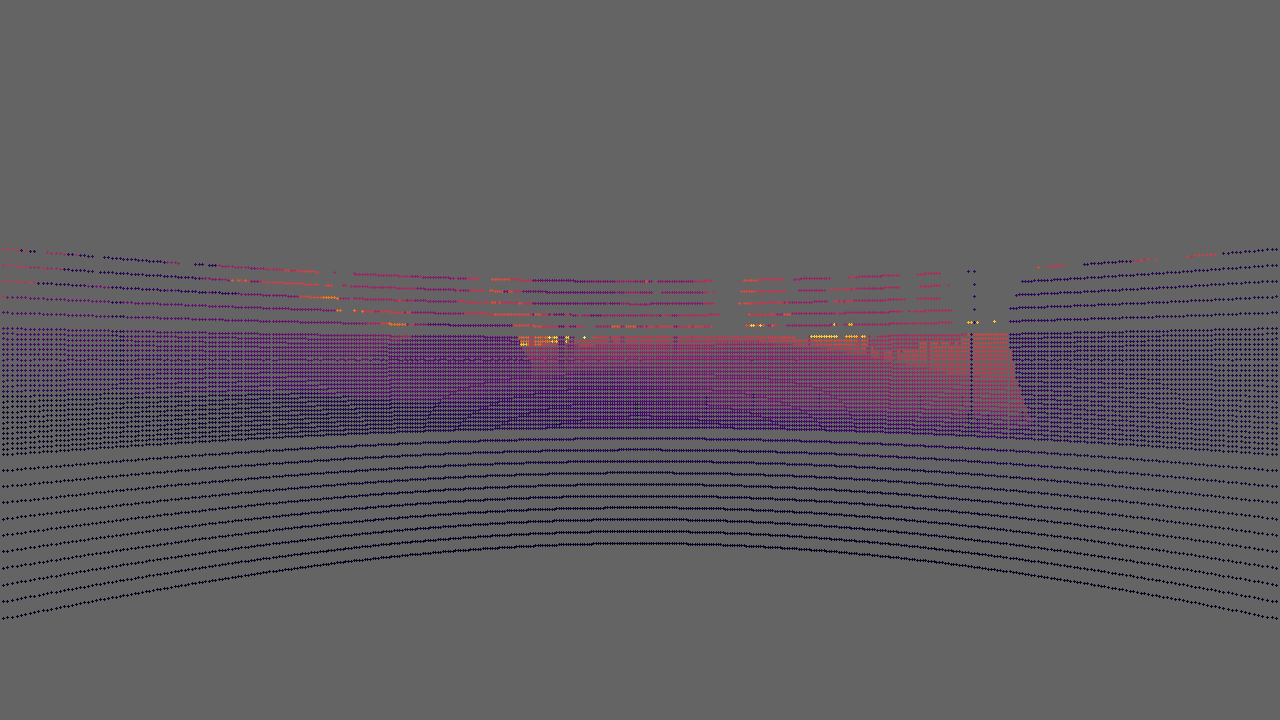
\includegraphics[width=\linewidth]{mainmatter/figures/5_depth_transf/sparse_network_cmp/lidar_lightgray_fixed.png}
    \subcaption{LiDAR projection}\label{subfig:delta:sparse_network_cmp:lidar}
  \end{subfigure}
  \begin{subfigure}{0.49\linewidth}
    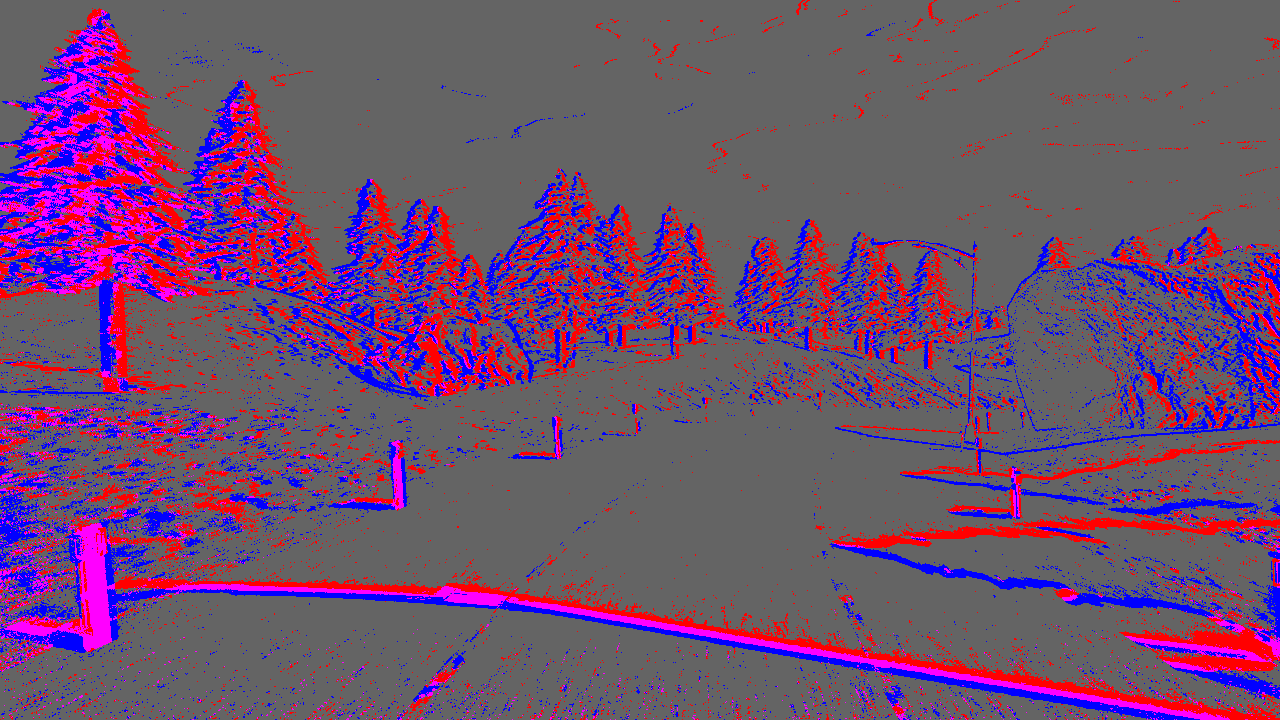
\includegraphics[width=\linewidth]{mainmatter/figures/5_depth_transf/sparse_network_cmp/events_lightgray_fixed.png}
    \subcaption{Events}\label{subfig:delta:sparse_network_cmp:evts}
  \end{subfigure}
  \begin{subfigure}{0.49\linewidth}
    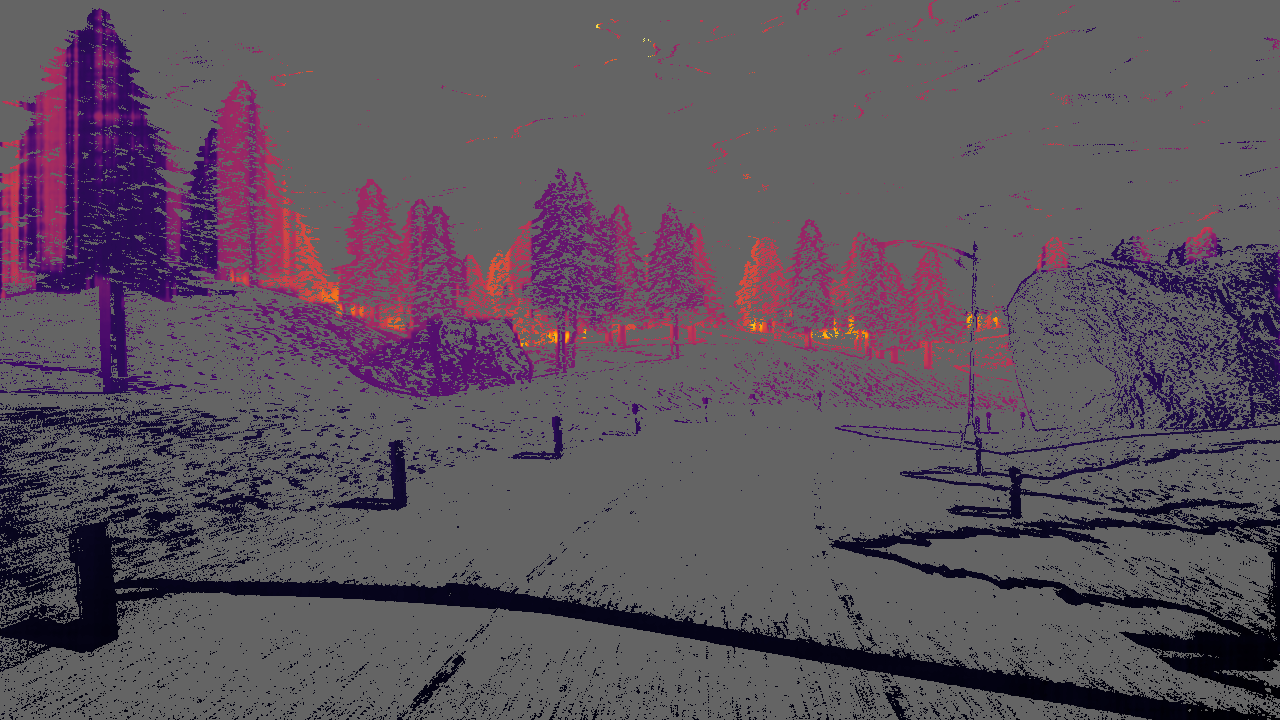
\includegraphics[width=\linewidth]{mainmatter/figures/5_depth_transf/sparse_network_cmp/predbf_lightgray_fixed.png}
    \subcaption{Prediction of the network}\label{subfig:delta:sparse_network_cmp:pred}
  \end{subfigure}
  \begin{subfigure}{0.49\linewidth}
    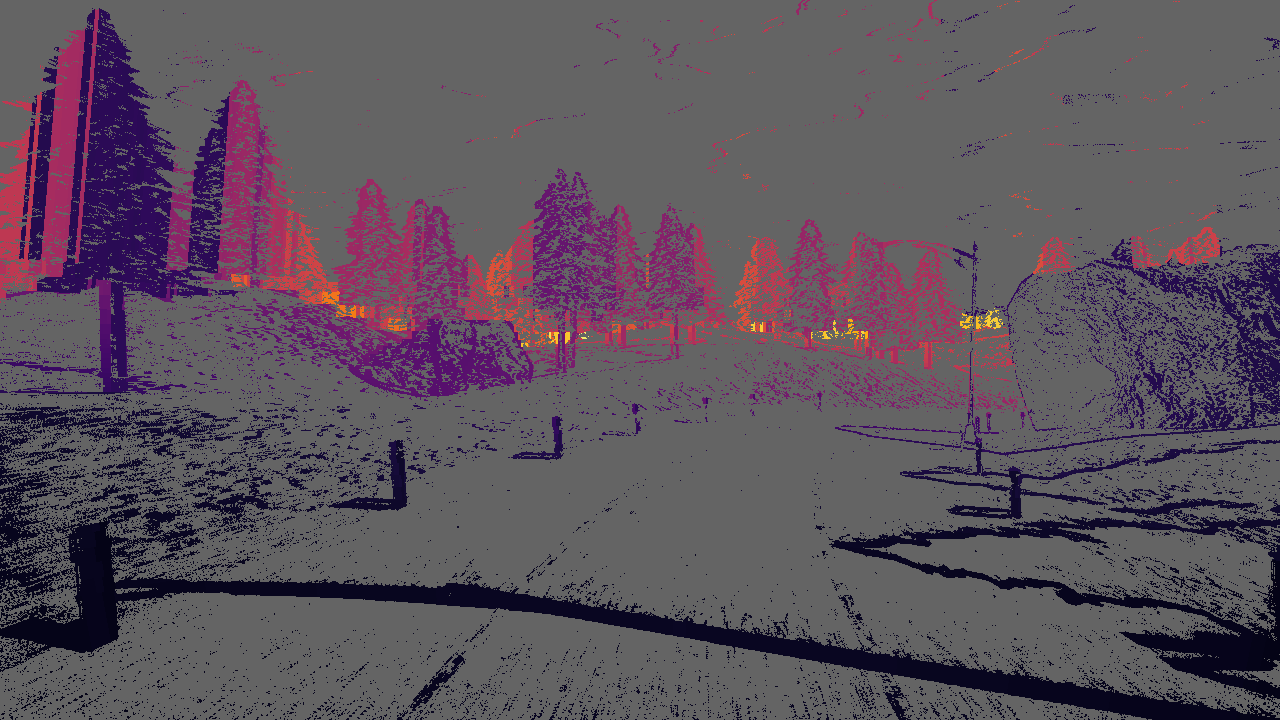
\includegraphics[width=\linewidth]{mainmatter/figures/5_depth_transf/sparse_network_cmp/nn_lightgray_fixed.png}
    \subcaption{Prediction of the \acrshort{nn} method}\label{subfig:delta:sparse_network_cmp:nn}
  \end{subfigure}
  \begin{subfigure}{0.49\linewidth}
    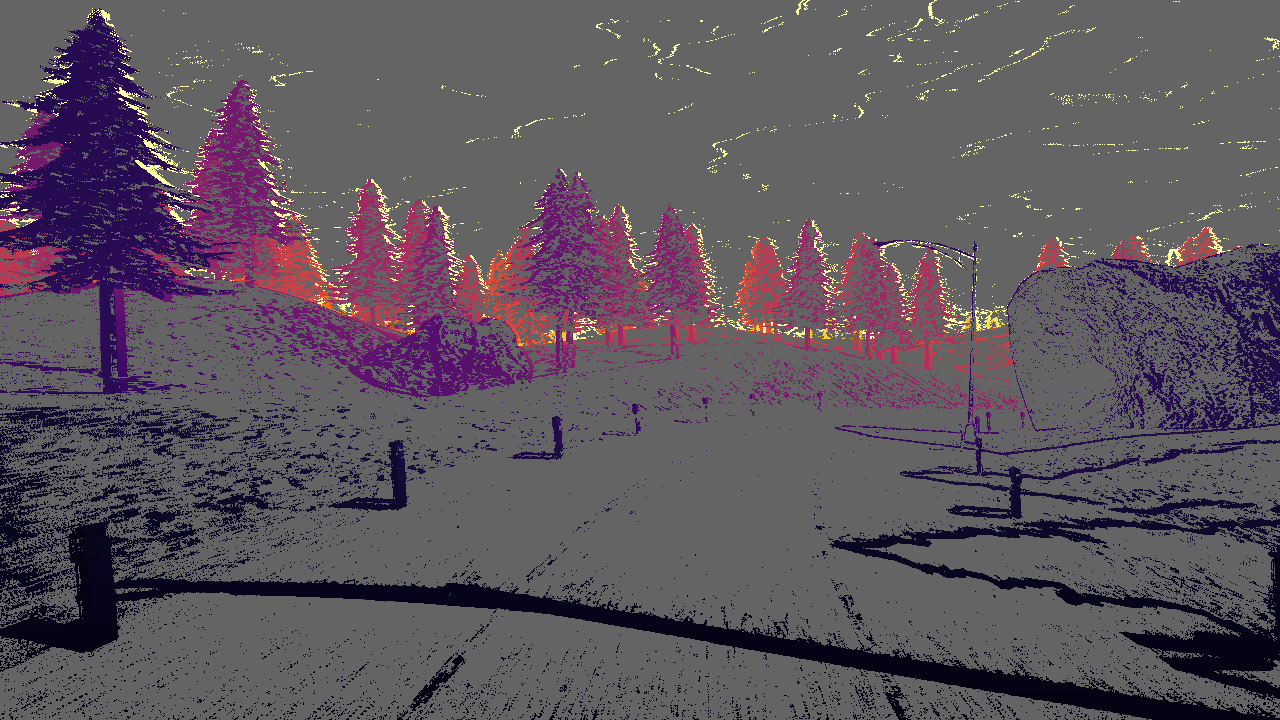
\includegraphics[width=\linewidth]{mainmatter/figures/5_depth_transf/sparse_network_cmp/gtbf_lightgray_fixed.png}
    \subcaption{Ground truth}\label{subfig:delta:sparse_network_cmp:gt}
  \end{subfigure}
  \caption{Results for the second version of our sparse network, for the previous depths \(d_\text{bf}\). As a reminder, the output of the network and of the \acrshort{nn} method is just a sequence of depths; we place them here in an image format for a better visualization.}\label{fig:delta:sparse_network_cmp}
\end{figure}

We display in \cref{fig:delta:sparse_network_cmp} example results achieved by the second version of the network after a complete training on our \acrshort{sled} dataset. As can be seen, while the depth association in \cref{subfig:delta:sparse_network_cmp:pred} is not catastrophic, it remains far from the ground truth: individual trees are not well separated, weird vertical artifacts appear (especially visible for the tree on the left), and events belonging to the sky (i.e., at the maximum distance, in pale yellow in the ground truth) are never identified as such. Actually, when observing the results produced by the simple \acrfull{nn} method in \cref{subfig:delta:sparse_network_cmp:nn}, the exact same issues appear, and the overall image looks strangely similar. This would indicate that our sparse attention-based network is only able to relate events and LiDAR points based on their spatial position like the \acrshort{nn} method, and that it has no real understanding of the content of the scene to correctly assign the depths.

\paragraph{Loss on Cross-Attention}\label{sec:delta:sparse_network:issues:loss_att}
Several attempts were made to improve the results of the network. The first main one was introducing a loss on the cross-attention during the training. The idea here was that supervising how events and LiDAR points are put in relation by the network would force it to stop going for the simple Nearest-Neighbor-like behavior, and instead force it to recognize patterns. However, this additional loss did not bring any improvement, as it only converged a little before the network reached its usual Nearest-Neighbor-like behavior, at which point it stopped converging. Attempts were made to give more importance to this loss, but always resulted in the divergence of the training process.

\paragraph{Maximum Distance Token}
Another element that was tested for improving the results was the introduction of a special ``maximum distance'' value, to fix the issue of events belonging to the sky never being identified as such. For the implementation, for each predicted depth, a secondary binary output was added, where the network would have to say whether or not the event should be placed at the maximum distance (and if so, the predicted depth would not be considered). Two different behaviors were observed here:
\begin{enumerate*}[label=\textbf{(\arabic*)}]
  \item in most cases, the network would mark all events as not being at the maximum distance, and would continue having the Nearest-Neighbor-like behavior as presented before;
  \item but in some cases, the network would consider that all events above a certain \(y\) value belonged to the sky, which while more interesting, still does not show a good understanding of the content of the scene, as this \(y\) value would not change during the full duration of a sequence, and as some objects like the top of the trees would be included in the sky. 
\end{enumerate*}

\subsection{Additional Experiments}
All the experiments described so far on a sparse depth estimation only constitute a fraction of all the tests that were conducted in the first part of the third year of thesis. Among all the other tests, we can list
\begin{itemize}
  \item a purely self-attention-based version of the network, where events and LiDAR points are concatenated as a single sequence directly after the encoding heads (with a different embedding added to each modality to allow the network to recognize them);
  \item a U-Net version of the network, where the event and LiDAR data would be progressively compressed during the encoding, and decompressed (with skip connections) during the decoding, allowing for more attention modules while decreasing memory usage;
  \item the test of more complex encoding and decoding heads;
  \item the addition of a special ``maximum range'' token to the LiDAR points, with a supervision of the cross-attention to force the events at maximum range to have a high attention score when associated to this token;
  \item the transformation of the maximum distance of the \acrshort{sled} dataset from 200m to 100m, meaning that more events are at that maximum distance in the ground truth, in the hope that the network would better learn about this special case.
\end{itemize}
Yet, none of these changes brought any improvement to the results presented in \cref{fig:delta:sparse_network_cmp}.


\section{Dense DELTA Method}\label{sec:delta:method}

\subsection{Switching to a Patch-Based Approach}
As shown in the previous section, the fully sparse version of the attention-based depth estimation network never yielded compelling results. Therefore, an important decision was taken: switching from this sparse depth estimation approach, for which the Transformer does not seem to be able to produce correct results, to a dense depth estimation approach, as in \cref{sec:aled}, where we expect the Transformer to be more suited.

For that purpose, we will reuse the concept of patches, as initially introduced by Dosovitskiy \textit{et al.} in their work on the Vision Transformer~\cite{Dosovitskiy2020AnII}, where their goal was to apply the Transformer on images. Their idea was to split each image into \(N_P\) small \((16\times{}16)\) patches, linearly project each patch as a single vector of dimensionality \(D\), add a positional encoding to differentiate each vector based on the position of the patch in the image, and use these vectors as the input sequence of shape \((N_P, D)\) to the Transformer. Compared to our sparse approach, each patch contains much more data than a single LiDAR point or a single event, conserves the local spatial and temporal structures of the data it contains, and results in a much more compact input representation of fixed size (from up to a million of events to only a few thousands of patches for \acrshort{hd} input), making the relations within and in-between the patches more simple for the network to learn.

While several iterations were required to achieve accurate results, we will only describe here the final version of the network for more clarity. Therefore, we propose in this chapter a novel attention-based recurrent network to estimate dense depth maps from LiDAR and event data. We call it \acrshort{delta}, for \acrlong{delta}.


\subsection{Architecture}\label{sec:delta:method:architecture}
As illustrated in \cref{fig:delta:network}, our network is based on a U-Net architecture~\cite{Ronneberger2015UNetCN}, with two input branches for frame-like representations of the LiDAR and accumulated event data, a central memory state, and a decoding branch. In total, \acrshort{delta} contains 180.9 million of trainable parameters.

\begin{figure}
  \centering

  % Defining the colors that will be used
  \definecolor{color_l}{RGB}{204,187,68}
  \definecolor{color_e}{RGB}{238,102,119}
  \definecolor{color_d}{RGB}{34,136,51}
  \definecolor{color_ca}{RGB}{68,119,170}
  \definecolor{color_sa}{RGB}{102,204,238}
  \definecolor{color_gru}{RGB}{187,187,187}
  \definecolor{color_sk}{RGB}{140,140,140}
  \definecolor{color_skd}{RGB}{170,51,119}

  \resizebox{\linewidth}{!}{
    \shorthandoff{:!}
    \begin{tikzpicture}[every node/.style={inner sep=0.001,outer sep=0.001,font=\normalsize}]
      % Changing the font
      \fontfamily{cmss}\selectfont

      % Helping grid
      %\draw[help lines] (0,0) grid (22,-16);

      % LiDAR encoding
      \node[] (L) at (0,0) {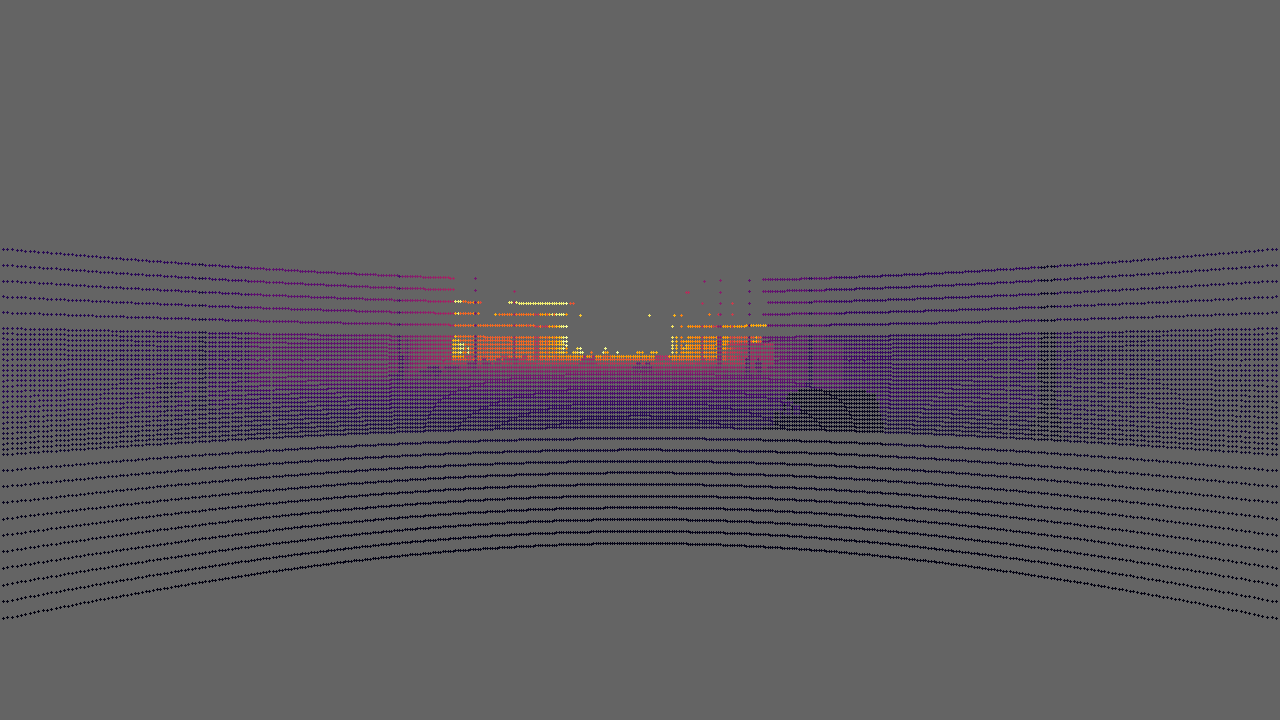
\includegraphics[height=2cm,cfbox=color_l 0.05cm 0pt]{mainmatter/figures/5_depth_transf/network/lidar005158_lightgray_fixed.png}};
      \node[above=0.1cm of L] (Ll) {\normalsize Input LiDAR};

      \node[draw, trapezium, minimum width=1.25cm, on grid, right=4.5cm of L, opacity=0.0] (tmplh) {};
      \node[draw, trapezium, fill=color_l, minimum width=1.25cm, rotate around={-90:(tmplh.center)}] (LH) at (tmplh) {};

      \node[draw, circle, minimum width=0.625cm, right=0.5cm of tmplh] (LP) {\Large +};

      \node[draw, fill=color_ca, rounded corners, minimum width=1cm, minimum height=1cm, right=2.25cm of LP] (LCA) {CA\textsubscript{P2}};

      \node[draw, fill=color_sa, rounded corners, minimum width=1cm, minimum height=1cm, right=3.25cm of LCA] (LSA1) {SA};

      \node[draw, fill=color_sa, rounded corners, minimum width=1cm, minimum height=1cm, right=1.5cm of LSA1] (LSA2) {SA};

      % Events encoding + propagation memory
      \node[below=2.9cm of L] (E) {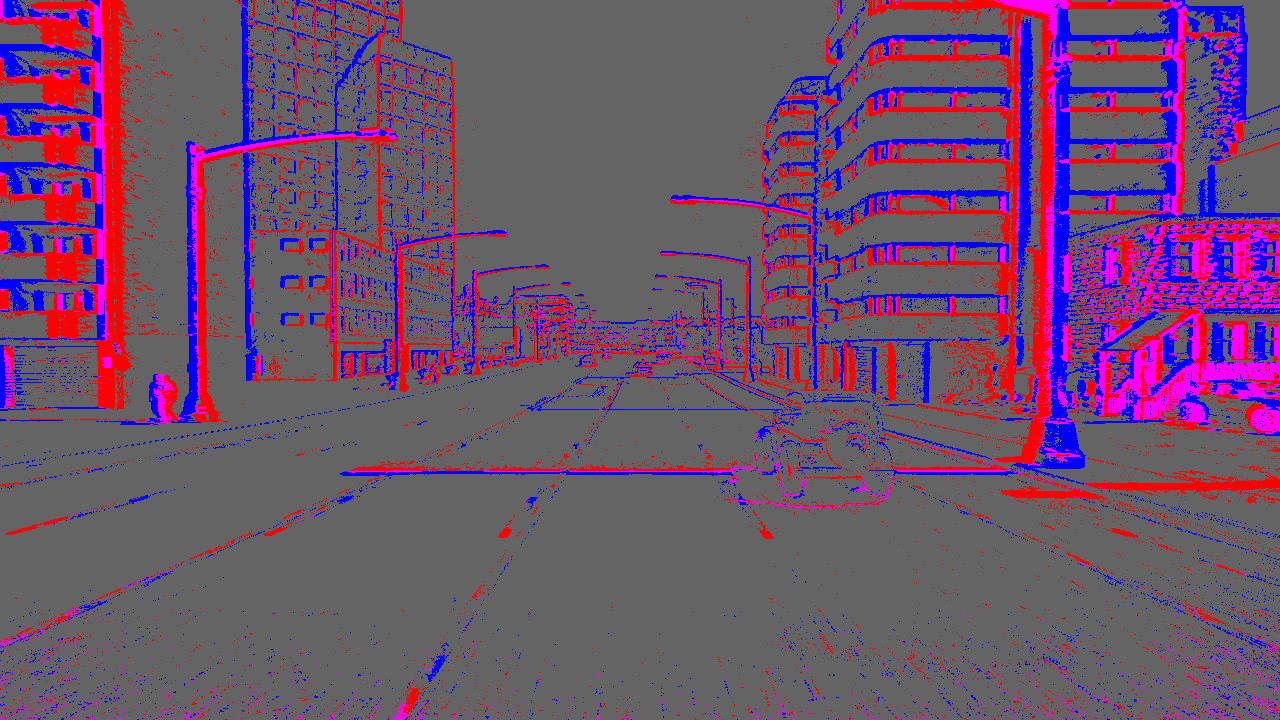
\includegraphics[height=2cm,cfbox=color_e 0.05cm 0pt]{mainmatter/figures/5_depth_transf/network/evts005158_lightgray_fixed.png}};
      \node[above=0.1cm of E] (El) {\normalsize Input Events};

      \node[draw, trapezium, minimum width=1.25cm, on grid, right=4.5cm of E, opacity=0.0] (tmpeh) {};
      \node[draw, trapezium, fill=color_e, minimum width=1.25cm, rotate around={-90:(tmpeh.center)}] (EH) at (tmpeh) {};

      \node[draw, circle, minimum width=0.625cm, right=0.5cm of tmpeh] (EP) {\Large +};

      \node[draw, fill=color_ca, rounded corners, minimum width=1cm, minimum height=1cm, below=2.6667cm of LCA] (PCA) {CA\textsubscript{P1}};

      \node[draw, minimum width=1cm, minimum height=1cm, above=0.8cm of PCA, align=center] (P) {Prop.\\mem.};

      \node[draw, fill=color_sa, rounded corners, minimum width=1cm, minimum height=1cm, below right=0.3333cm and 3.25cm of PCA] (ESA1) {SA};

      \node[draw, fill=color_sa, rounded corners, minimum width=1cm, minimum height=1cm, right=1.5cm of ESA1] (ESA2) {SA};

      % Positional encoding
      \node[draw, circle, minimum width=1cm, minimum height=1cm, between=LP and EP] (PE) {};
      \draw[thick] ($(PE)+(-0.5cm,0)$) sin ($(PE)+(-0.25cm,0.3cm)$) cos (PE) sin ($(PE)+(0.25cm,-0.3cm)$) cos ($(PE)+(0.5cm,0)$);

      % Central memory update
      \node[draw, fill=color_ca, rounded corners, minimum width=1cm, minimum height=1cm, below right=1.5cm and 0.75cm of LSA2] (MCA) {CA\textsubscript{F}};

      \node[draw, fill=color_gru, rounded corners, minimum width=1cm, minimum height=1cm, right=0.75cm of MCA] (MGRU) {GRU};

      \node[draw, minimum width=1cm, minimum height=1cm, right=0.75cm of MGRU, align=center] (M) {Cent.\\mem.};

      % Decoding
      \node[draw, fill=color_sa, rounded corners, minimum width=1cm, minimum height=1cm, on grid, below=3.5cm of ESA2] (DSA2) {SA};

      \node[draw, fill=color_sa, rounded corners, minimum width=1cm, minimum height=1cm, left=1.5cm of DSA2] (DSA1) {SA};

      \node[draw, trapezium, minimum width=1.25cm, on grid, below=3.5cm of tmpeh, opacity=0.0] (tmpdh) {};
      \node[draw, trapezium, fill=color_d, minimum width=1.25cm, rotate around={-90:(tmpdh.center)}] (DH) at (tmpdh) {};

      \node[on grid, left=4.5cm of tmpdh] (D) {
        \begin{tikzpicture}
          \node[on grid] (Daf) {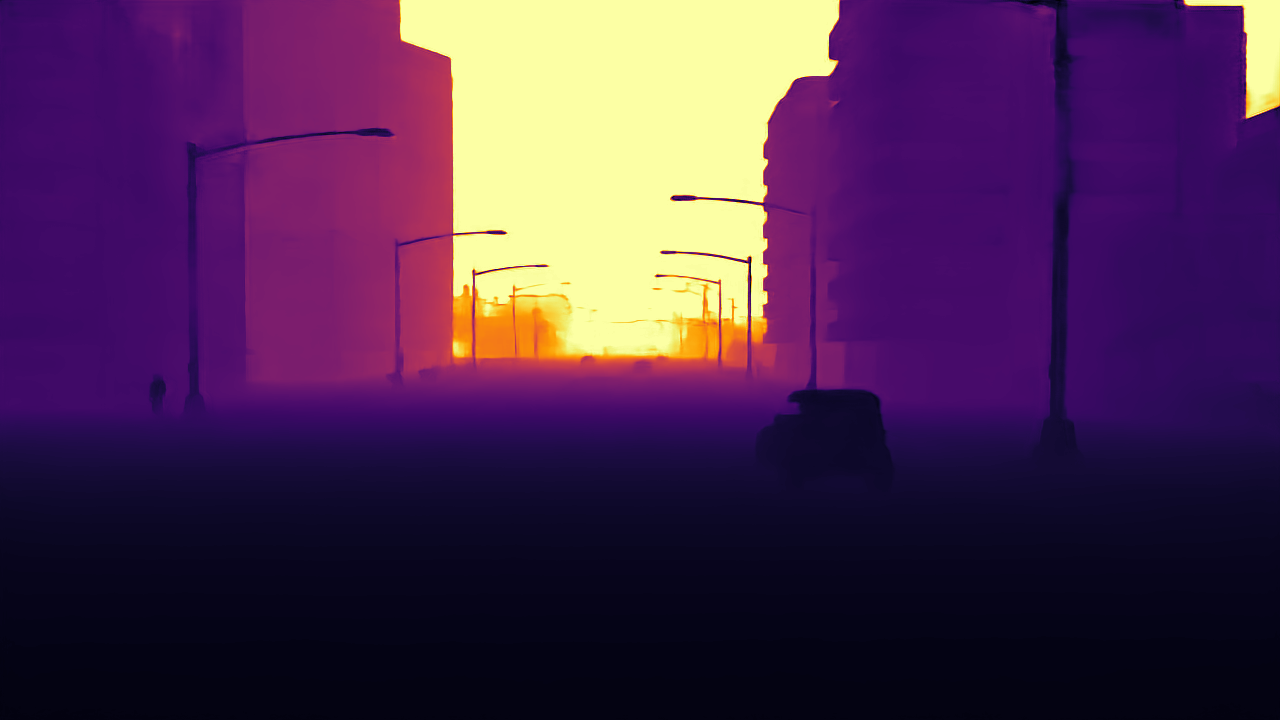
\includegraphics[height=1.85cm,cfbox=color_d 0.05cm 0pt]{mainmatter/figures/5_depth_transf/network/predaf005158.png}};
          \node[on grid, below left=0.25cm and 0.25cm of Daf] (Dbf) {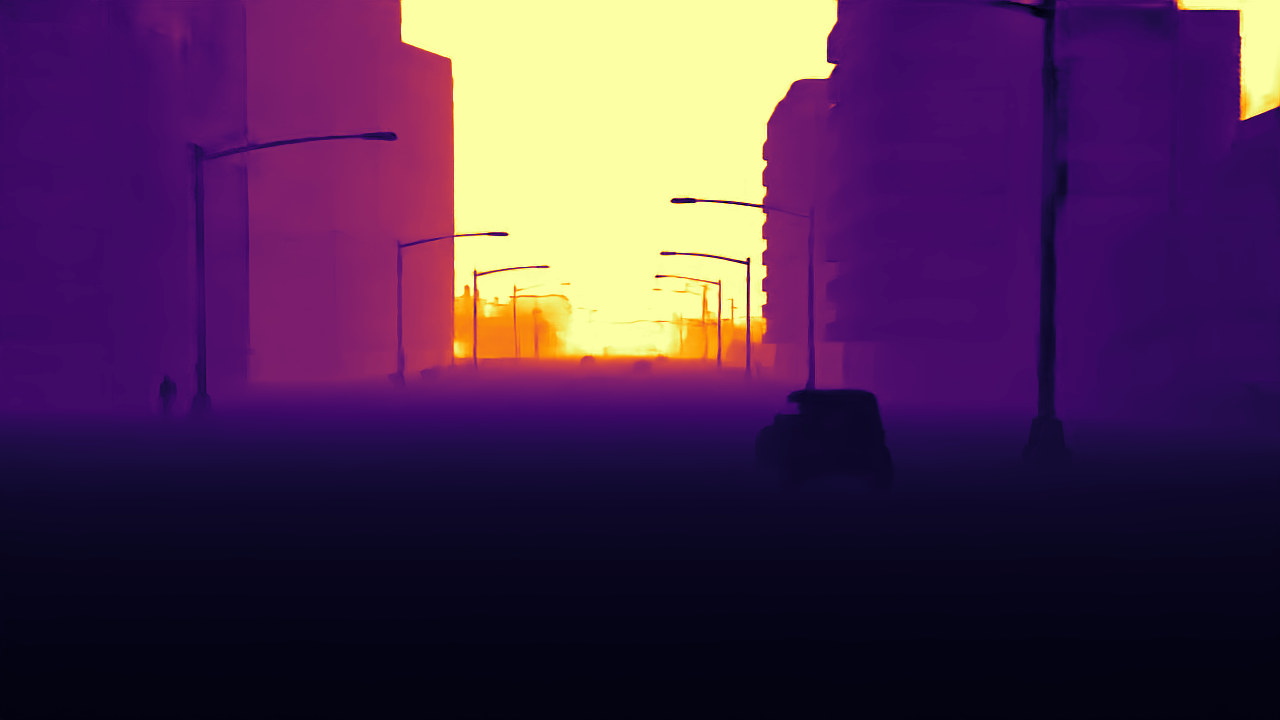
\includegraphics[height=1.85cm,cfbox=color_d 0.05cm 0pt]{mainmatter/figures/5_depth_transf/network/predbf005158.png}};
        \end{tikzpicture}
      };
      \node[above=0.1cm of D] (Dl) {\normalsize Output Depth Maps};

      % Skip connections (SA)
      \node[draw, circle, color_sk, minimum width=0.625cm, below left=1.6875cm and 0.75cm of LSA1] (SP1a) {\Large +};
      \node[draw, circle, color_sk, minimum width=0.625cm, below left=1.6875cm and 0.75cm of LSA2] (SP2a) {\Large +};
      \node[draw, circle, color_sk, minimum width=0.625cm, left=0.25cm of DSA1] (SP1b) {\Large +};
      \node[draw, circle, color_sk, minimum width=0.625cm, left=0.25cm of DSA2] (SP2b) {\Large +};

      % Paths
      \draw[dashed, color_sk, ->, >=latex, line width=0.5mm] (ESA1.west -| SP1a) -- (SP1a);
      \draw[dashed, color_sk, ->, >=latex, line width=0.5mm] (ESA2.west -| SP2a) -- (SP2a);
      \draw[dashed, color_sk, ->, >=latex, line width=0.5mm] (LSA1.west -| SP1a) -- (SP1a);
      \draw[dashed, color_sk, ->, >=latex, line width=0.5mm] (LSA1.west -| SP2a) -- (SP2a);
      \draw[dashed, color_sk, ->, >=latex, line width=0.5mm] (SP1a) -| (SP1b);
      \draw[dashed, color_sk, ->, >=latex, line width=0.5mm] (SP2a) -| (SP2b);
      \draw[dashdotted, color_skd, ->, >=latex, line width=0.5mm] (EH) -- (DH);

      \draw[->,>=latex, line width=0.5mm, color_l] (L) -- node [above=0.1cm, midway] (al) {(B, H, W, 1)} (LH);
      \draw[->,>=latex, line width=0.5mm, color_l] (LH) -- (LP);
      \draw[->,>=latex, line width=0.5mm, color_l] (LP) -- node [above=0.1cm, pos=0.85] (aplq) {\color{color_ca} \textbf{Q}} (LCA);
      \draw[->,>=latex, line width=0.5mm, color_e] (LCA) -- (LSA1);
      \draw[->,>=latex, line width=0.5mm, dashed, color_l] (LCA) -- (LSA1);
      \draw[->,>=latex, line width=0.5mm, color_e] (LSA1) -- (LSA2);
      \draw[->,>=latex, line width=0.5mm, dashed, color_l] (LSA1) -- (LSA2);
      \draw[->,>=latex, line width=0.5mm, color_e] (LSA2) -| node [left=0.1cm, pos=0.95] (amkv) {\color{color_ca} \textbf{K/V}} (MCA);
      \draw[->,>=latex, line width=0.5mm, dashed, color_l] (LSA2) -| (MCA);

      \draw[->,>=latex, line width=0.5mm, color_e] (E) -- node [above=0.1cm, midway] (ae) {(B, H, W, 4)} (EH);
      \draw[->,>=latex, line width=0.5mm, color_e] (EH) -- (EP);
      \draw[->,>=latex, line width=0.5mm, color_e] (EP -| PCA) -- node [left=0.1cm, pos=0.7] (apkv) {\color{color_ca} \textbf{K/V}} (PCA);
      \draw[->,>=latex, line width=0.5mm, color_e] (EP) -- (ESA1);
      \draw[->,>=latex, line width=0.5mm, color_e] (ESA1) -- (ESA2);
      \draw[->,>=latex, line width=0.5mm, color_e] (ESA2) -| node [left=0.1cm, pos=0.935] (amq) {\color{color_ca} \textbf{Q}} (MCA);

      \draw[->,>=latex, line width=0.5mm] (PE) -- (LP);
      \draw[->,>=latex, line width=0.5mm] (PE) -- (EP);

      \draw[->,>=latex, line width=0.5mm, color_e] ([xshift=-0.2cm] P.south) -- node [left=0.1cm, pos=0.75] (apq) {\color{color_ca} \textbf{Q}} node [left=0.1cm, pos=0.3] (apq2) {(B, 128, D)} ([xshift=-0.2cm] PCA.north);
      \draw[->,>=latex, line width=0.5mm, color_e] ([xshift=0.2cm] PCA.north) -- node [right=0.1cm] (apo) {(B, 128, D)} ([xshift=0.2cm] P.south);
      \draw[->,>=latex, line width=0.5mm, color_e] (P) -- node [left=0.1cm, pos=0.7] (aplkv) {\color{color_ca} \textbf{K/V}} node [right=0.1cm] (aplkv2) {(B, 128, D)} (LCA);

      \draw[->,>=latex, line width=0.5mm] (MCA) -- (MGRU);
      \draw[->,>=latex, line width=0.5mm] ([yshift=0.2cm] M.west) -- ([yshift=0.2cm] MGRU.east);
      \draw[->,>=latex, line width=0.5mm] ([yshift=-0.2cm] MGRU.east) -- ([yshift=-0.2cm] M.west);

      \draw[->,>=latex, line width=0.5mm, color_d] (M) |- (DSA2);
      \draw[->,>=latex, line width=0.5mm, color_d] (DSA2) -- (SP2b);
      \draw[->,>=latex, line width=0.5mm, color_d] (SP2b) -- (DSA1);
      \draw[->,>=latex, line width=0.5mm, color_d] (DSA1) -- (SP1b);
      \draw[->,>=latex, line width=0.5mm, color_d] (SP1b) -- (DH);
      \draw[->,>=latex, line width=0.5mm, color_d] (DH) -- node [above=0.1cm, midway] (ad) {(B, H, W, 2)} (D);

      % Separation between network and legend
      \draw[line width=0.6mm] ($(D.south west)+(-0.5cm,-1cm)$) -- ($(D.south west)+(23.75cm,-1cm)$);

      % Legend title
      \node[align=center, below right=1.75cm and 10cm of D.south west] (Title) {\Large\textbf{Legend}};

      % Legend for Encoding heads
      \node[draw, trapezium, minimum width=1cm, below left=1.25cm and 10.5cm of Title, opacity=0.0] (tmplh) {};
      \node[draw, trapezium, fill=color_l, minimum width=1cm, rotate around={-90:(tmplh.center)}] (LH) at (tmplh) {};

      \node[draw, trapezium, minimum width=1cm, right=0cm of tmplh, opacity=0.0] (tmpeh) {};
      \node[draw, trapezium, fill=color_e, minimum width=1cm, rotate around={-90:(tmpeh.center)}] (EH) at (tmpeh) {};

      \node[align=center, right=0.3cm of tmpeh] (HEl) {\normalsize Convolutional\\\normalsize encoding heads};

      % Legend for Decoding head
      \node[draw, trapezium, minimum width=1cm, on grid, below left=1.25cm and -0.075cm of tmpeh.south west, opacity=0.0] (tmpdh) {};
      \node[draw, trapezium, fill=color_d, minimum width=1cm, rotate around={-90:(tmpdh.center)}] (DH) at (tmpdh) {};

      \node[align=center, right=0.775cm of tmpdh] (HDl) {\normalsize Convolutional\\\normalsize decoding head};

      % Legend for Cross-attention
      \node[draw, fill=color_ca, rounded corners, minimum width=1cm, minimum height=1cm, right=1.5cm of HEl] (CA) {CA};

      \node[align=center, right=0.5cm of CA] (CAl) {\normalsize Cross-attention\\\normalsize module};

      % Legend for Self-attention
      \node[draw, fill=color_sa, rounded corners, minimum width=1cm, minimum height=1cm, on grid, below=0.75cm of CA.south] (SA) {SA};

      \node[align=center, right=0.7cm of SA] (SAl) {\normalsize Self-attention\\\normalsize module};

      % Legend for Positional encoding
      \node[draw, circle, minimum width=1cm, minimum height=1cm, right=1.5cm of CAl] (PE) {};
      \draw[thick] ($(PE)+(-0.5cm,0)$) sin ($(PE)+(-0.25cm,0.3cm)$) cos (PE) sin ($(PE)+(0.25cm,-0.3cm)$) cos ($(PE)+(0.5cm,0)$);

      \node[align=center, right=0.8cm of PE] (PEl) {\normalsize Positional\\\normalsize embedding};

      % Legend for GRU
      \node[draw, fill=color_gru, rounded corners, minimum width=1cm, minimum height=1cm, on grid, below=0.75cm of PE.south] (GRU) {GRU};

      \node[align=center, right=0.5cm of GRU] (GRUl) {\normalsize Gated Recurrent\\\normalsize Unit module};

      % Legend for Propagation memory
      \node[draw, align=center, minimum width=1cm, minimum height=1cm, right=1.5cm of PEl] (P) {Prop.\\mem.};

      \node[align=center, right=0.75cm of P] (Pl) {\normalsize Propagation\\\normalsize memory};

      % Legend for Central memory
      \node[draw, align=center, minimum width=1cm, minimum height=1cm, on grid, below=0.75cm of P.south] (M) {Cent.\\mem.};

      \node[align=center, right=1.1cm of M] (Ml) {\normalsize Central\\\normalsize memory};

      % Legend for Skip connections
      \node[minimum width=1cm, minimum height=1cm, right=1.5cm of Pl] (S) {};
      \draw[dashed, color_sk, ->, >=latex, line width=0.5mm] (S.west) -- (S.east);

      \node[align=center, right=0.8cm of S] (Sl) {\normalsize Skip\\\normalsize connections};

      % Legend for Evts for guiding the decoding
      \node[minimum width=1cm, minimum height=1cm, on grid, below=0.75cm of S.south] (G) {};
      \draw[dashdotted, color_skd, ->, >=latex, line width=0.5mm] (G.west) -- (G.east);

      \node[align=center, right=0.95cm of G] (Gl) {\normalsize Decoding\\\normalsize guide};
    \end{tikzpicture}
    \shorthandon{:!}
  }

  \caption{The complete architecture of our \acrshort{delta} network. Unless noted, data is of shape \((B, N_P, D)\), where \(B\) is the batch size, \(N_P\) is the number of patches, and \(D\) is the dimensionality.}\label{fig:delta:network}
\end{figure}

\paragraph{Encoding heads}
As explained earlier, the event and LiDAR data (both of shape \((H, W, C)\), where \(C\) is the number of channels) are first split into small patches of size \(P\times{}P\), as originally proposed by Dosovitskiy \textit{et al.}~\cite{Dosovitskiy2020AnII}. This process is done through stacked \(5\times{}5\) convolutional layers, and results in data of shape \((N_P, D)\), where \(N_P\) is the number of patches, and \(D = P\times{}P\times{}C\) the dimensionality of each patch. These encoded patches are then summed with a fixed 2-dimensional positional embedding, following the formulation of Carion \textit{et al.}~\cite{Carion2020EndtoEndOD}. This way, each patch has its own unique signature, making the network able to distinguish them.

\paragraph{Data encoding and fusion}
Both the event and LiDAR patches each go through two self-attention modules, to encode the internal relations between their own patches. A cross-attention module (CA\textsubscript{F} in \cref{fig:delta:network}) is then used to encode the cross-relations of both the event and LiDAR patches, with the encoded events being the queries and the encoded LiDAR being the keys/values (as we want in the end to obtain depth maps, similarly to the sparse network of \cref{fig:delta:sparse_network_v2}).

\paragraph{LiDAR propagation}
Due to the use of this cross-attention module, contrary to the work proposed in \cref{sec:aled}, our LiDAR and event branches can not be totally decorrelated, as both LiDAR and event data are necessary at each time step. On the basis that event data might be more frequently available than LiDAR point clouds, unless new LiDAR data is available, we propagate at each time step the previous LiDAR data using the incoming events. To do so, the events are used to update a small (\cref{sec:delta:eval:impl_detail:memory_size}) propagation memory via a cross-attention module (CA\textsubscript{P1} in \cref{fig:delta:network}). As before, the memory is the queries (i.e., it ``asks'' how its values should be updated), and the events are the keys/values (i.e., the events provide the new propagation model). This propagation memory is then used in a second cross-attention module (CA\textsubscript{P2}), where the previous LiDAR data is the queries, and where the propagation memory serves as the keys/values, in order to output an updated LiDAR representation.

\paragraph{Memory update}\label{sec:method:memory}
Considering the case where the event camera and the LiDAR are placed on a dynamic platform (e.g., a road vehicle), then if that platform was to come to a halt (e.g., at an intersection or in a traffic jam), few to no event would be produced by the camera. As such, densifying the LiDAR would become a difficult task, as the events would not be able to provide the guiding information required. To solve this issue, given the sequential nature of the inputs, we add a central state, whose role is to give a memory effect to the network. This way, even if the event camera and LiDAR become static, the network can still exploit the memory of the previous information from these sensors to derive accurate predictions. Additionally, the use of this memory state has the benefit of stabilizing the output of the network. Regarding the implementation, the fused LiDAR and event data are given to a \acrfull{gru} module, which updates this central memory.

\paragraph{Decoding}
To obtain the final depth maps, the data from the central memory first passes through two self-attention modules, each followed by a skip connection with the corresponding summed and normalized LiDAR and event data from the encoding branch. To be able to have an image-like output, a final decoding head is used to regroup the decoded patches and reshape the data to its original size. This decoding head is composed of stacked convex upsampling modules~\cite{Teed2020RAFTRA}, where the upsampling is guided by the corresponding data from the events encoding head. The output is of shape \((H, W, 2)\), where the ``before'' depth map \(D_\text{bf}\) is in the first channel, and the ``after'' depth map \(D_\text{af}\) is in the second channel. 

\subsection{Loss Functions}
To train \acrshort{delta}, we use the exact same two complementary losses as in \cref{sec:aled}, \cref{sec:aled:method:loss}: the pixel-wise \(\ell_1\) loss \(\mathcal{L}_\text{pw}\), and the multiscale gradient-matching loss \(\mathcal{L}_\text{msg}\). Both losses are applied here with the same weights, as we did not observe any improvement by giving more importance to one or the other. Our final loss \(\mathcal{L}\) is therefore a summation of both these losses over a full sequence of predictions of length \(T\):
\begin{equation}
  \mathcal{L} = \sum_{t=1}^T \sum_{\text{bf}, \text{af}} (\mathcal{L}_\text{pw}^t + \mathcal{L}_{\text{msg}}^t).
\end{equation}


\section{Evaluation}\label{sec:delta:eval}

\subsection{Datasets}
To conduct the training and evaluation of \acrshort{delta}, we use in this chapter both our \acrshort{sled} dataset and the MVSEC dataset~\cite{Zhu2018TheMS}, as in the previous chapter. For a more complete evaluation, we also use the M3ED dataset~\cite{Chaney2023M3EDMM}. However, due to its size, and since its authors do not provide any LiDAR data for the test set, we can not use it as is. To still be able to provide insightful results, we subsampled the dataset and redefined the train/validation/test sets as shown in \cref{tab:delta:split_m3ed}.

\begin{table}[ht]
  \centering
  \resizebox{\linewidth}{!}{
    \begin{tabular}{@{}lcr@{}}
      \toprule
      Redefined set & Recordings & Total length \\
      \midrule
      Train & \Verb|penno_small_loop_day|; \Verb|rittenhouse_day|; \Verb|penno_small_loop_night| & 8m02s \\
      Val & \Verb|horse_day|; \Verb|ucity_small_loop_night| & 8m59s \\
      Test & \Verb|city_hall_day|; \Verb|city_hall_night| & 9m43s \\
      \bottomrule
    \end{tabular}
  }
  \caption{M3ED sets used within this chapter.}\label{tab:delta:split_m3ed}
\end{table}

\subsection{Implementation Details}
\paragraph{Data representation}\label{sec:delta:eval:impl_detail:data_repres}
The event data is split in temporal windows of fixed size \(\Delta t\), based on the rate of the ground truth of each dataset (\(\Delta t = 50\text{ms}\) for \acrshort{sled} and MVSEC, \(\Delta t = 100\text{ms}\) for M3ED). The events in each window are then accumulated into an Event Volume of shape \((H, W, 4)\), following the formulation of Zhu \textit{et al.}~\cite{Zhu2019UnsupervisedEL}. Compared to \acrshort{aled}, where the formulation of Perot \textit{et al.}~\cite{Perot2020LearningTD} was used, the formulation of Zhu \textit{et al.} is more compact, by not separating the polarities of the events, allowing for their data to be fully kept by our network while limiting the memory usage, as will be explained in the next paragraph. As for the LiDAR point clouds, they are represented as their projection on the event camera's image plane. Pixels without any depth value are set to 0. Both the LiDAR projections and ground truth depth maps are normalized between 0 and 1, where 1 is the maximum LiDAR range in the dataset in use.

\paragraph{Data size}
To reach a patch size \(P\) of 16 pixels, we use five convolutional layers in the encoding heads, and four convex upsampling modules in the decoding head. To be able to keep all data intact, we chose to use \mbox{\(D = 1024\)}, as each patch from the event data contains \(16 \times 16 \times 4 = 1024\) elements (patch size \texttimes{} number of channels of an Event Volume), and as using greater values of \(D\) would raise the memory usage too high. During training, data is randomly cropped to a size of \(512 \times 512\) pixels for the high-resolution \acrshort{sled} and M3ED datasets, and to \(256 \times 256\) pixels for the low-resolution MVSEC dataset.

\paragraph{Memories size and initialization}\label{sec:delta:eval:impl_detail:memory_size}
Since the role of the central memory is to condense past data, its shape must be the same as the rest of the data in the network, i.e., \((N, D)\). On the contrary, the propagation memory is only a parametric representation of how the LiDAR data should be propagated to match the current events. While its dimensionality is still constrained to \(D\), its number of elements \(N\) can be tuned: we empirically chose a size of \(128\) in this work. As for their initialization, the central memory is initialized with a copy of the two-dimensional positional embedding, while the initial state of the propagation memory is learned.

\paragraph{Training details}
For training on all datasets, we use the Adam optimizer~\cite{Kingma2015AdamAM} with a batch size \(B = 4\). When training from scratch on the \acrshort{sled} and the M3ED datasets, 50 epochs are used, the initial learning rate is set to \(10^{-4}\), and it is decayed by \(0.01^{1/49}\) after each epoch (in order to reach a learning rate of \(10^{-6}\) at the last epoch). When training from scratch on the MVSEC dataset, 20 epochs are used, and the learning rate is set to a constant value of \(10^{-4}\). When finetuning on MVSEC or M3ED, 3 epochs are used, and the learning rate is set to \(10^{-5}\).

\paragraph{Evaluation metrics}
For all datasets, we use the same metrics for dense and sparse evaluation as in \cref{sec:aled}. Following the convention on the MVSEC dataset~\cite{Zhu2018TheMS}, results in the following subsections will also be presented with various cutoff distances (10m, 20m, 30m, half the maximum range, and the maximum range). As for \acrshort{aled}, \acrshort{delta} is trained on the full depth maps, i.e., at the maximum range, and these cutoffs are only applied at test time.

\subsection{Results on the SLED Dataset}\label{sec:delta:eval:results_sled}
We begin by training the network solely on the \acrshort{sled} dataset, and denote this version DELTA\textsubscript{SL}. Results of DELTA\textsubscript{SL} on the testing set of \acrshort{sled} are presented in \cref{tab:delta:results_sled}, compared with those of ALED\textsubscript{SL} originally given in \cref{tab:aled:results_sled}.

\begin{table}[ht]
  \centering
  \resizebox{\linewidth}{!}{
    \begin{tabular}{@{}clccccccccccc@{}}
      \addlinespace[-\aboverulesep]
      \cmidrule[\heavyrulewidth]{2-13}
      \multirow{13}[5]{*}{\rotatebox[origin=c]{90}{\large \textbf{ALED\textsubscript{SL}}}} & & \multirow{3}[3]{*}{\textbf{Cutoff}} & \multicolumn{4}{c}{\textbf{Dense depths errors}} & \multicolumn{4}{c}{\textbf{Sparse depths errors}} & \multicolumn{2}{c}{\textbf{Depth change map errors}} \\ \cmidrule(lr){4-7} \cmidrule(lr){8-11} \cmidrule(lr){12-13}
      & & & \multicolumn{2}{c}{On \(D_\text{bf}\)} & \multicolumn{2}{c}{On \(D_\text{af}\)} & \multicolumn{2}{c}{On \(D_\text{bf}\)} & \multicolumn{2}{c}{On \(D_\text{af}\)} & \multirow{2}[1]{*}{Mean (m)} & Correctly classified events (\%) \\ \cmidrule(lr){4-5} \cmidrule(lr){6-7} \cmidrule(lr){8-9} \cmidrule(lr){10-11}
      & & & Mean (m) & AbsRel & Mean (m) & AbsRel & NN (m) & ALED\textsubscript{SL} (m) & NN (m) & ALED\textsubscript{SL} (m) & & (with a threshold of \rpm{}1m) \\
      \cmidrule{2-13}
      & \multirow{5}{*}{\Verb|Town01|} & 10m & 1.24 & 0.201 & 1.37 & 0.236 & 1.32 & 1.46 & 2.24 & 1.79 & \textbf{2.11} & 90.27 \\
      & & 20m & 2.08 & 0.231 & 2.27 & 0.255 & 1.51 & 1.84 & 2.53 & 2.15 & 3.18 & 85.07 \\
      & & 30m & 2.72 & 0.238 & 2.92 & 0.260 & 1.71 & 2.37 & 2.83 & 2.67 & \textbf{3.88} & 81.68 \\
      & & 100m & 4.25 & 0.240 & 4.51 & 0.261 & 2.40 & 3.48 & 3.91 & 3.95 & \textbf{5.12} & 77.48 \\
      & & 200m & \textbf{4.53} & 0.172 & \textbf{4.81} & 0.187 & 7.86 & \textbf{5.44} & 9.76 & \textbf{6.23} & \textbf{7.36} & 75.54 \\
      \cmidrule{2-13}
      & \multirow{5}{*}{\Verb|Town03|} & 10m & 2.00 & 0.289 & 2.09 & 0.301 & 0.47 & 0.56 & 0.67 & 0.66 & 1.14 & 93.70 \\
      & & 20m & 2.85 & 0.299 & 2.97 & 0.311 & 0.64 & 0.75 & 1.12 & 0.87 & 2.54 & 87.16 \\
      & & 30m & 3.33 & 0.291 & 3.45 & 0.302 & 0.92 & 1.11 & 1.61 & 1.26 & 3.23 & 83.71 \\
      & & 100m & 4.60 & 0.274 & 4.77 & 0.284 & 1.88 & 2.55 & 3.17 & 2.88 & 4.47 & 78.50 \\
      & & 200m & 4.86 & 0.215 & 5.03 & 0.223 & 4.43 & 3.60 & 5.93 & 4.10 & \textbf{6.20} & 77.23 \\
      \cmidrule[\heavyrulewidth]{2-13}
      \addlinespace[-\belowrulesep]
      \\
      \addlinespace[-\aboverulesep]
      \cmidrule[\heavyrulewidth]{2-13}
      \multirow{13}[5]{*}{\rotatebox[origin=c]{90}{\large \textbf{DELTA\textsubscript{SL}}}} & & \multirow{3}[3]{*}{\textbf{Cutoff}} & \multicolumn{4}{c}{\textbf{Dense depths errors}} & \multicolumn{4}{c}{\textbf{Sparse depths errors}} & \multicolumn{2}{c}{\textbf{Depth change map errors}} \\ \cmidrule(lr){4-7} \cmidrule(lr){8-11} \cmidrule(lr){12-13}
      & & & \multicolumn{2}{c}{On \(D_\text{bf}\)} & \multicolumn{2}{c}{On \(D_\text{af}\)} & \multicolumn{2}{c}{On \(D_\text{bf}\)} & \multicolumn{2}{c}{On \(D_\text{af}\)} & \multirow{2}[1]{*}{Mean (m)} & Correctly classified events (\%) \\ \cmidrule(lr){4-5} \cmidrule(lr){6-7} \cmidrule(lr){8-9} \cmidrule(lr){10-11}
      & & & Mean (m) & AbsRel & Mean (m) & AbsRel & NN (m) & DELTA\textsubscript{SL} (m) & NN (m) & DELTA\textsubscript{SL} (m) & & (with a threshold of \rpm{}1m) \\
      \cmidrule{2-13}
      & \multirow{5}{*}{\Verb|Town01|} & 10m & \textbf{0.64} & \textbf{0.101} & \textbf{0.67} & \textbf{0.105} & 1.32 & \textbf{1.14} & 2.24 & \textbf{1.25} & 2.19 & \textbf{91.81} \\
      & & 20m & \textbf{1.45} & \textbf{0.138} & \textbf{1.50} & \textbf{0.144} & 1.51 & \textbf{1.62} & 2.53 & \textbf{1.74} & \textbf{3.17} & \textbf{87.81} \\
      & & 30m & \textbf{2.11} & \textbf{0.155} & \textbf{2.17} & \textbf{0.161} & 1.71 & \textbf{2.03} & 2.83 & \textbf{2.15} & \textbf{3.88} & \textbf{84.45} \\
      & & 100m & \textbf{3.80} & \textbf{0.174} & \textbf{3.89} & \textbf{0.179} & 2.40 & \textbf{3.05} & 3.91 & \textbf{3.24} & 5.14 & \textbf{79.86} \\
      & & 200m & 5.37 & \textbf{0.133} & 5.42 & \textbf{0.136} & 7.86 & 6.04 & 9.76 & 6.24 & 7.94 & \textbf{77.47} \\
      \cmidrule{2-13}
      & \multirow{5}{*}{\Verb|Town03|} & 10m & \textbf{0.49} & \textbf{0.081} & \textbf{0.50} & \textbf{0.082} & 0.47 & \textbf{0.36} & 0.56 & \textbf{0.40} & \textbf{0.76} & \textbf{97.35} \\
      & & 20m & \textbf{1.15} & \textbf{0.107} & \textbf{1.18} & \textbf{0.109} & 0.64 & \textbf{0.58} & 1.12 & \textbf{0.64} & \textbf{2.31} & \textbf{91.84} \\
      & & 30m & \textbf{1.72} & \textbf{0.121} & \textbf{1.77} & \textbf{0.124} & 0.92 & \textbf{0.90} & 1.61 & \textbf{0.98} & \textbf{3.06} & \textbf{88.35} \\
      & & 100m & \textbf{3.12} & \textbf{0.133} & \textbf{3.18} & \textbf{0.136} & 1.88 & \textbf{2.25} & 3.17 & \textbf{2.38} & \textbf{4.30} & \textbf{82.88} \\
      & & 200m & \textbf{4.81} & \textbf{0.114} & \textbf{4.81} & \textbf{0.116} & 4.43 & \textbf{3.54} & 5.93 & \textbf{3.72} & 6.69 & \textbf{81.18} \\
      \cmidrule[\heavyrulewidth]{2-13}
      \addlinespace[-\belowrulesep]
    \end{tabular}
  }
  \caption{Errors of ALED\textsubscript{SL} (top) and of DELTA\textsubscript{SL} (bottom) on our \acrshort{sled} dataset for various cutoff depth distances. From left to right: dense depth errors (absolute and relative) on the full \(D_\text{bf}\) and \(D_\text{af}\) depth maps; sparse depth errors (only pixels with events are considered); absolute depth change maps (\(D_\text{af}-D_\text{bf}\)) errors and percentage of correctly classified events based on this depth difference.}\label{tab:delta:results_sled}
\end{table}

Compared to the results of ALED\textsubscript{SL}, a clear improvement can be seen across all metrics. Improvement is particularly important for the close objects, as the average raw errors at the 10m cutoff is divided by 2 and by 4 for the \verb|Town01| and \verb|Town03| maps respectively. Improvement is less significant at longer ranges, but as noted in the conclusion of \cref{sec:aled} (\cref{sec:aled:conclusion}), close surroundings of the robot are more important when operating than distant objects.

Errors on sparse depths (i.e., depths given to each event) are also much better than those of ALED\textsubscript{SL}. Despite only being trained on dense data, these errors often surpass those of the simpler Nearest Neighbor (NN) approach, which was not the case for ALED\textsubscript{SL} on the ``before'' depth maps \(D_\text{bf}\).

Errors between the \(D_\text{bf}\) and the \(D_\text{af}\) depth maps are also more consistent. Regarding the depth change maps, errors are often better than those of ALED\textsubscript{SL}, and the classification of events based on them (whether or not they belong to the edge of an object) is better for all cutoff distances. All these observations indicate that our network has an overall better learning of the temporal propagation of the depths.

\begin{figure}
  \centering
  \setlength\tabcolsep{1pt}
  \renewcommand{\arraystretch}{0.5}
  \begin{tabular}{@{}ccc@{}}
    \raisebox{2cm}[0pt][0pt]{\rotatebox[origin=c]{90}{Ground truth}} &
    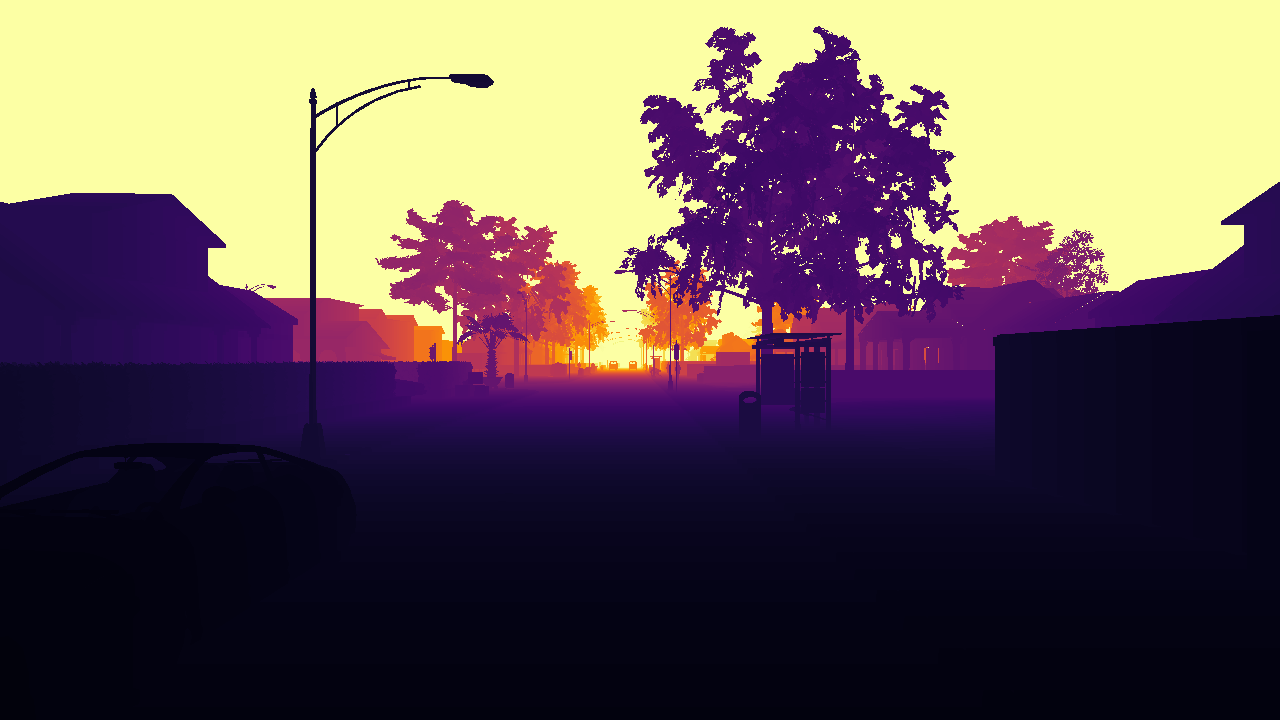
\includegraphics[width=0.475\linewidth]{mainmatter/figures/5_depth_transf/sled_cmp/data_and_gt/gtprev001662.png} &
    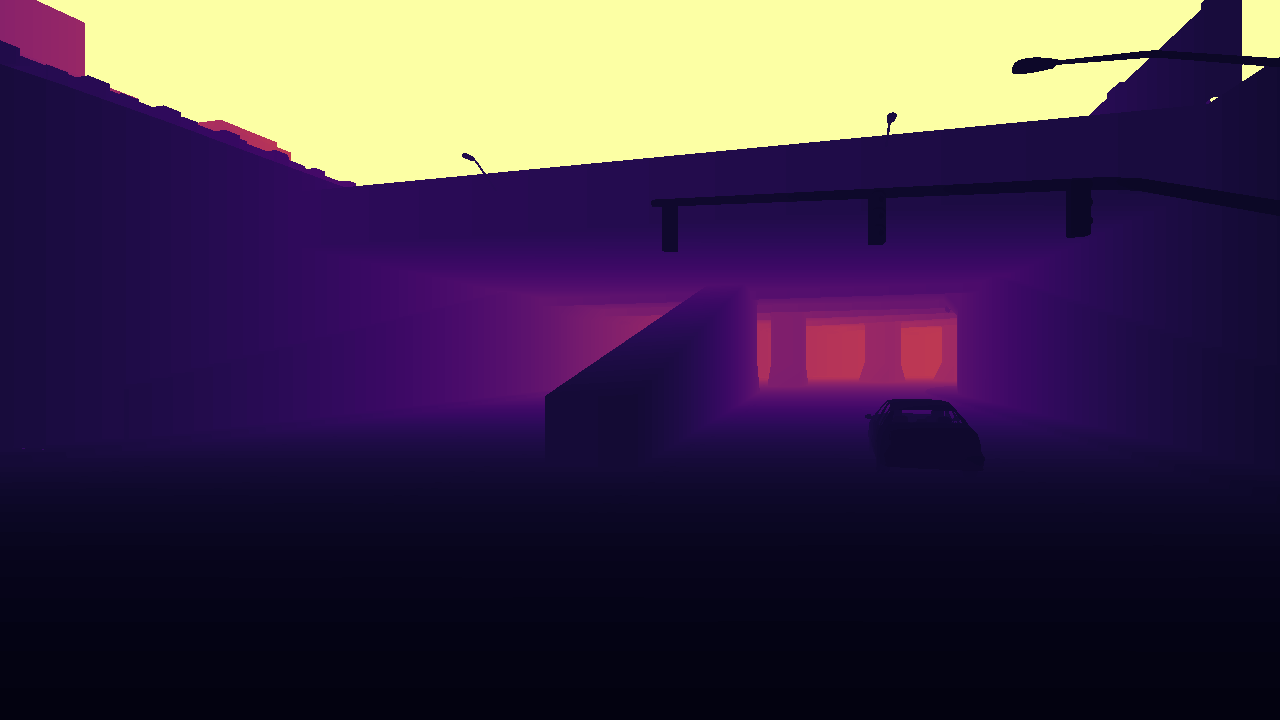
\includegraphics[width=0.475\linewidth]{mainmatter/figures/5_depth_transf/sled_cmp/data_and_gt/gtprev007812.png} \\
    \raisebox{2cm}[0pt][0pt]{\rotatebox[origin=c]{90}{ALED\textsubscript{SL}}} &
    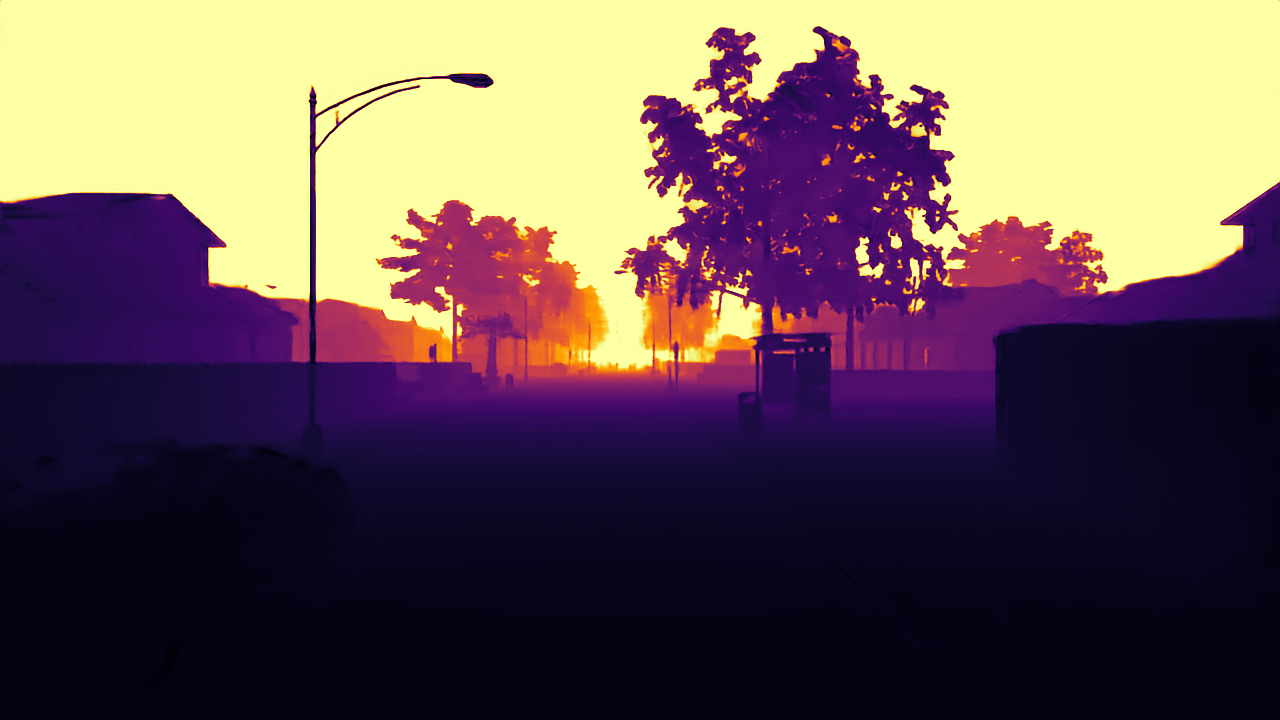
\includegraphics[width=0.475\linewidth]{mainmatter/figures/5_depth_transf/sled_cmp/aled/prev001662.png} &
    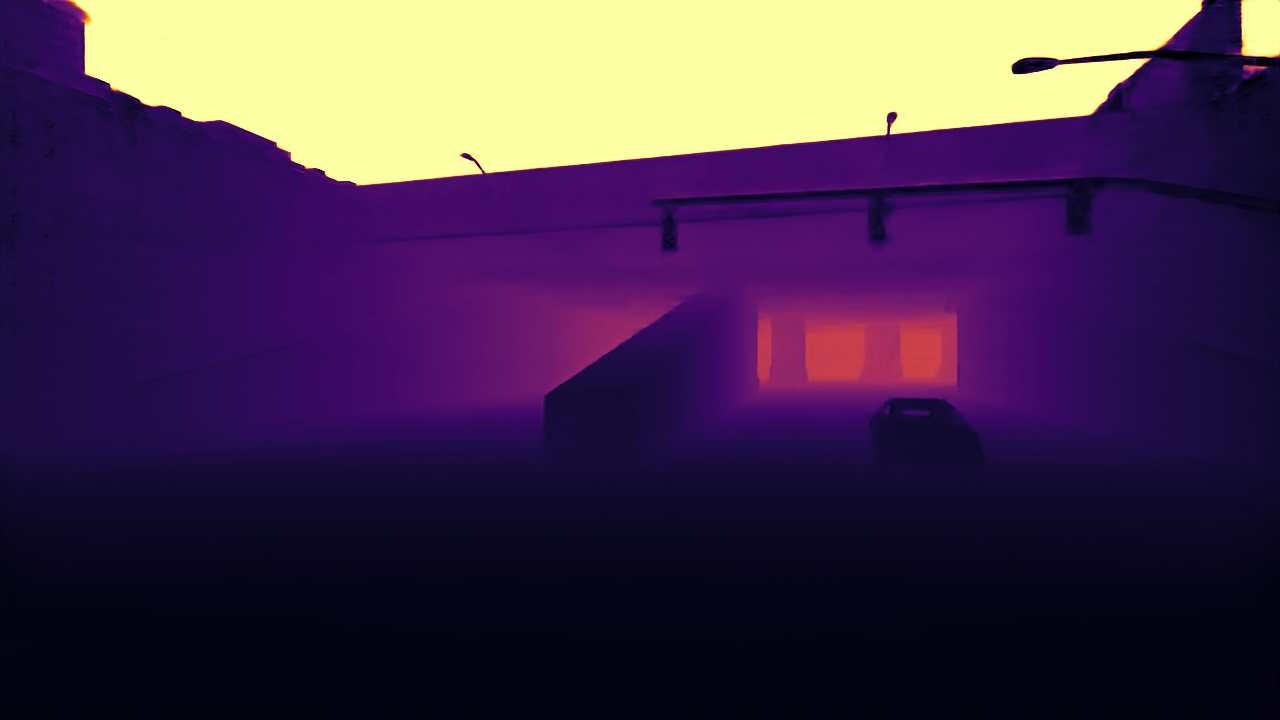
\includegraphics[width=0.475\linewidth]{mainmatter/figures/5_depth_transf/sled_cmp/aled/prev007812.png} \\
    \raisebox{2cm}[0pt][0pt]{\rotatebox[origin=c]{90}{DELTA\textsubscript{SL}}} &
    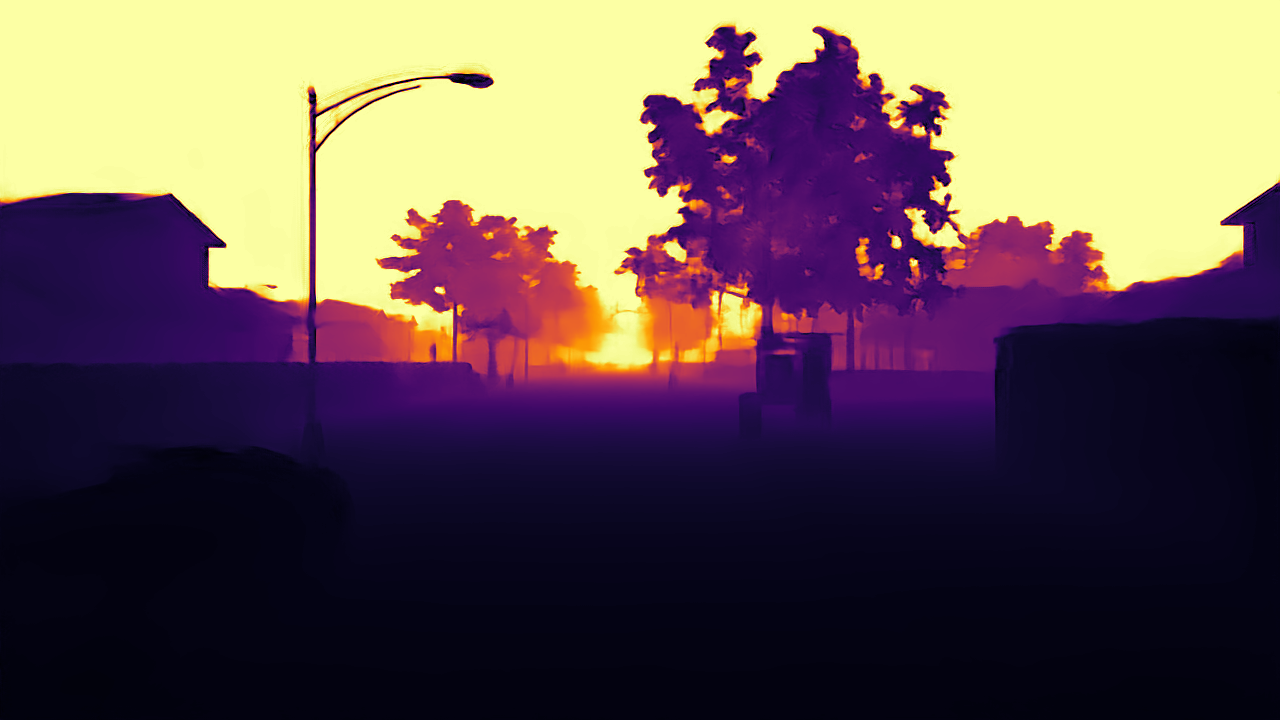
\includegraphics[width=0.475\linewidth]{mainmatter/figures/5_depth_transf/sled_cmp/delta/predbf001662.png} &
    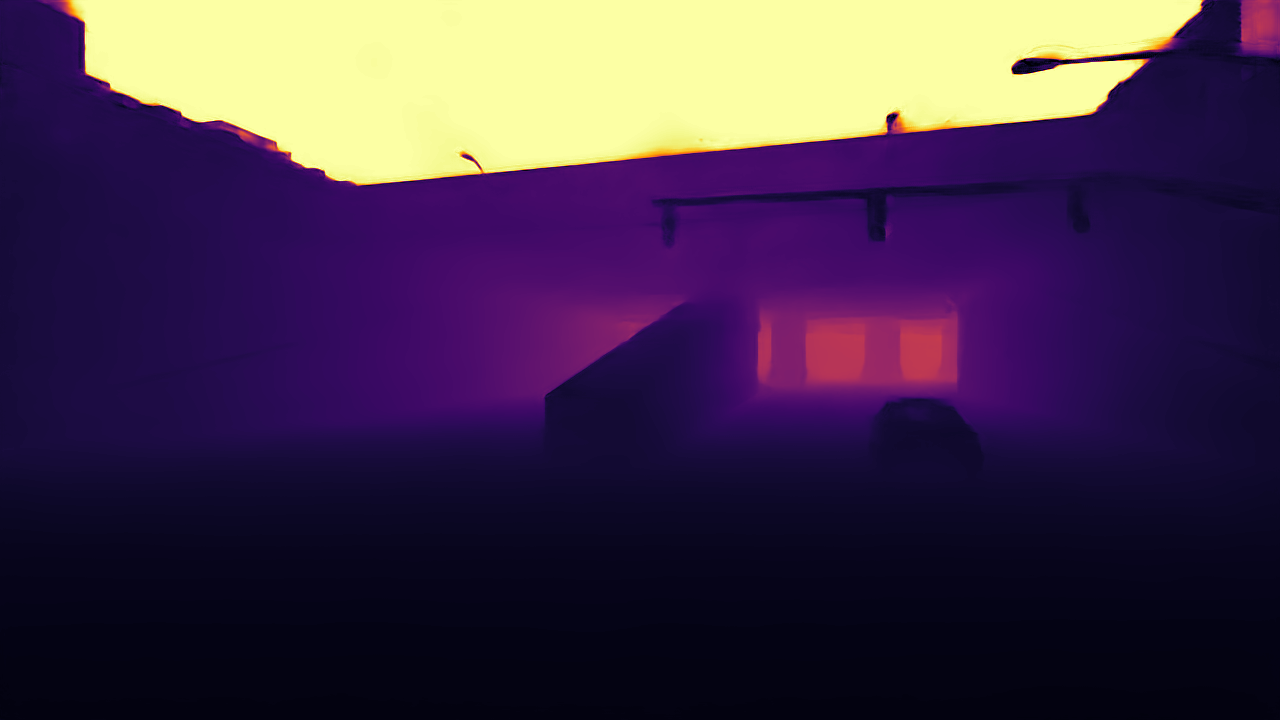
\includegraphics[width=0.475\linewidth]{mainmatter/figures/5_depth_transf/sled_cmp/delta/predbf007812.png} \\
    \raisebox{2cm}[0pt][0pt]{\rotatebox[origin=c]{90}{Errors ALED\textsubscript{SL}}} &
    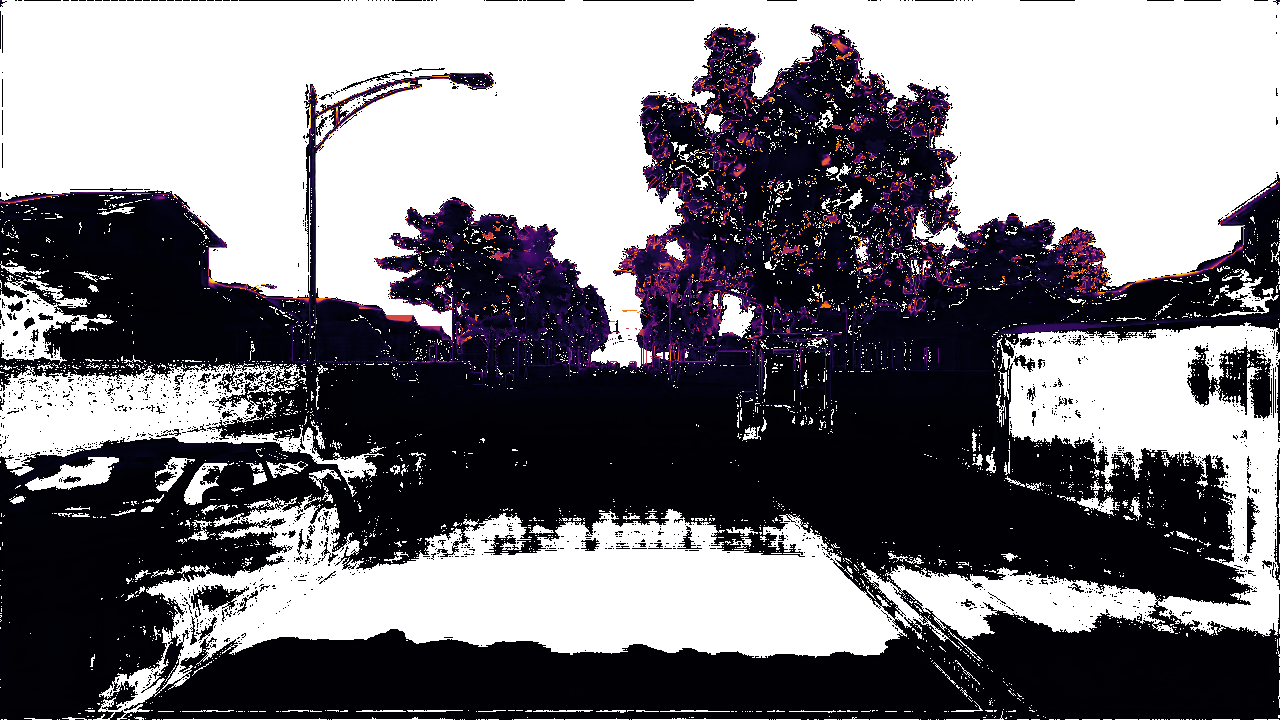
\includegraphics[width=0.475\linewidth]{mainmatter/figures/5_depth_transf/sled_cmp/aled/errorbf001662.png} &
    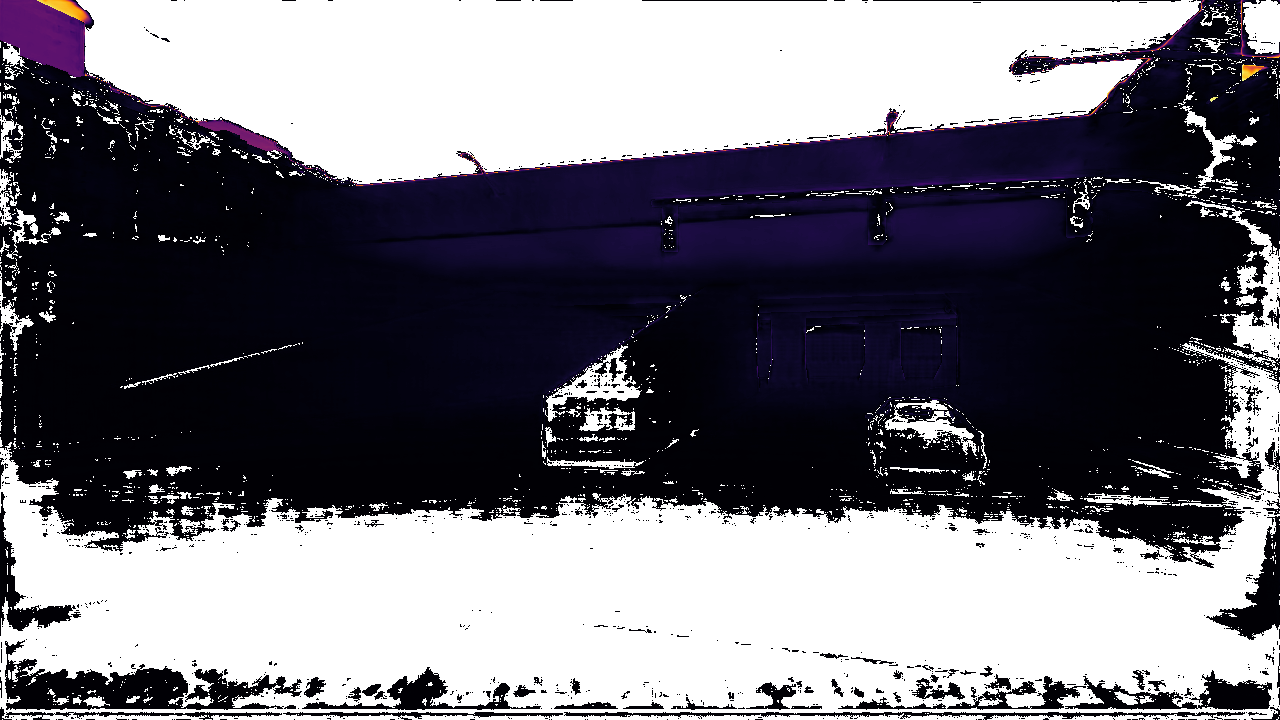
\includegraphics[width=0.475\linewidth]{mainmatter/figures/5_depth_transf/sled_cmp/aled/errorbf007812.png} \\
    \raisebox{2cm}[0pt][0pt]{\rotatebox[origin=c]{90}{Errors DELTA\textsubscript{SL}}} &
    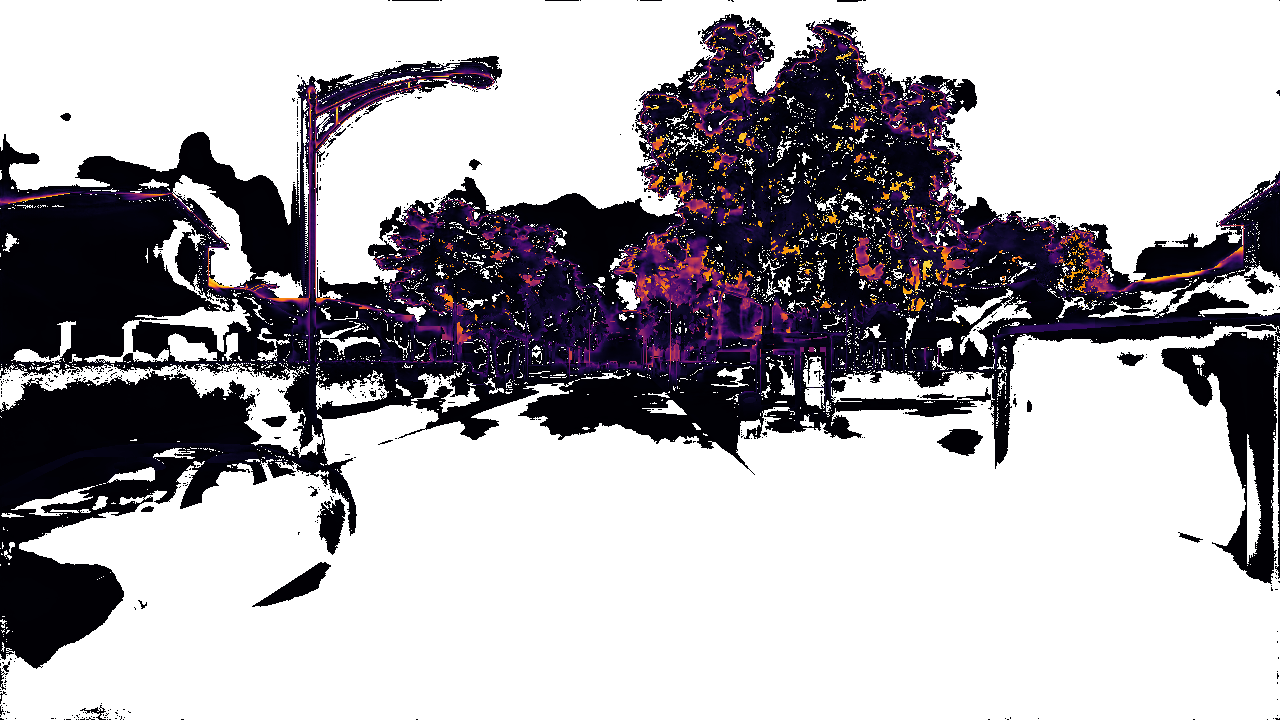
\includegraphics[width=0.475\linewidth]{mainmatter/figures/5_depth_transf/sled_cmp/delta/errorbf001662.png} &
    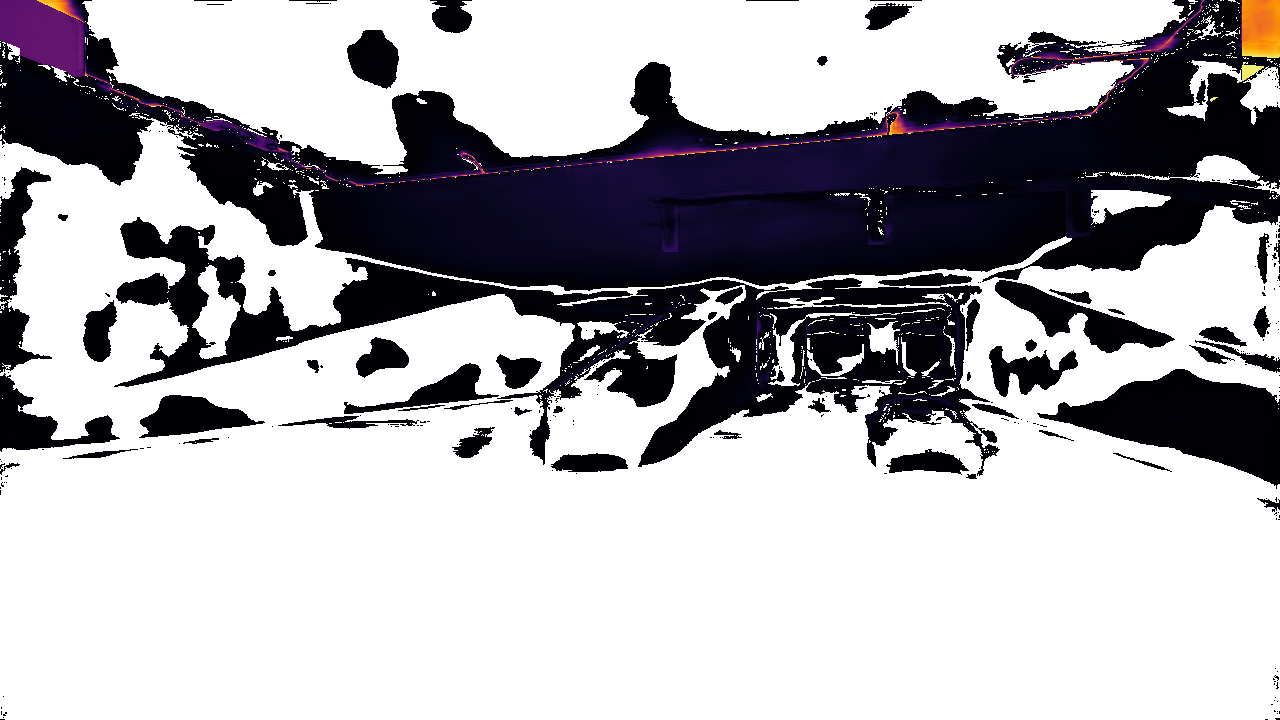
\includegraphics[width=0.475\linewidth]{mainmatter/figures/5_depth_transf/sled_cmp/delta/errorbf007812.png}
  \end{tabular}
  \cprotect\caption{Results on the \verb|Town01_08| (left) and \verb|Town03_19| (right) sequences of our \acrshort{sled} dataset, for the ``before'' depth map \(D_\text{bf}\). From top to bottom: ground truth depth map; result from ALED\textsubscript{SL}; result from DELTA\textsubscript{SL}; error maps of both methods, where pixels with an error inferior to 0.5m are in white.}\label{fig:delta:cmp_sled}
\end{figure}

Visual results are also presented in \cref{fig:delta:cmp_sled}. Looking at the predicted depth maps, our network is able to infer accurate results, close to the ground truth, but with edges looking less sharp than the ones of \acrshort{aled}. Looking at the error maps, they confirm the observations made on the quantitative results: we commit very small errors at close ranges (especially for the ground) and larger errors at longer ranges, and \acrshort{aled} commits small errors over the whole depth map.

If the reader is interested, the full numerical results for each sequence of the testing set and more visual results are both given in \cref{sec:appendix:delta:sled_full,sec:appendix:delta:visual_results_sled} respectively, and results in video format are available through the link given at the very beginning of this chapter (\cpageref{sec:delta}).

\subsection{Results on the MVSEC Dataset}
As for \acrshort{aled}, to evaluate our network on the MVSEC dataset, we follow two distinct strategies:
\begin{itemize}
  \item we only train it on MVSEC, noted as DELTA\textsubscript{MV}, and 
  \item we reuse the weights trained on the \acrshort{sled} dataset, DELTA\textsubscript{SL}, and finetune them on the MVSEC dataset: we denote it as DELTA\textsubscript{SL\(\rightarrow\)MV}.
\end{itemize}
The results of both versions are given in \cref{tab:delta:results_mvsec}, in addition to the results of other methods of the state of the art.

\begin{table}[ht]
  \centering
  \resizebox{\linewidth}{!}{
    \begin{tabular}{@{}cccccccccc@{}}
      \toprule
      \multirow{2}[1]{*}{\textbf{Recording}} & \multirow{2}[1]{*}{\textbf{Cutoff}} & \textbf{Events (stereo)} & \multicolumn{2}{c}{\textbf{Events \& Frames}} & \multicolumn{5}{c}{\textbf{Events \& LiDAR}} \\ \cmidrule(lr){3-3} \cmidrule(lr){4-5} \cmidrule(lr){6-10}
      & & StereoSpike~\cite{Ranon2021StereoSpikeDL} & RAMNet~\cite{Gehrig2021CombiningEA} & EvT\textsuperscript{+}~\cite{Sabater2022EventTA+} & Cui \textit{et al.}~\cite{Cui2022DenseDE} & ALED\textsubscript{MV} & \textbf{DELTA\textsubscript{MV}} & ALED\textsubscript{SL\(\rightarrow\)MV} & \textbf{DELTA\textsubscript{SL\(\rightarrow\)MV}} \\
      \midrule
      \multirow{5}{*}{\Verb|outdoor_day_1|} & 10m & 0.79 & 1.39 & 1.24 & 1.24 & 0.91 & 0.74 & \textbf{0.50} & \underline{0.59} \\
      & 20m & 1.47 & 2.17 & 1.91 & 1.28 & 1.22 & 1.10 & \textbf{0.80} & \underline{0.93} \\
      & 30m & 1.92 & 2.76 & 2.36 & 4.87 & 1.43 & 1.34 & \textbf{1.02} & \underline{1.17} \\
      & 50m & - & - & - & - & 1.67 & 1.65 & \textbf{1.31} & \underline{1.46} \\
      & 100m & 3.17 & - & - & - & 1.96 & 1.98 & \textbf{1.60} & \underline{1.79} \\
      \midrule
      \multirow{5}{*}{\Verb|outdoor_night_1|} & 10m & \textbf{1.38} & 2.50 & \underline{1.45} & 2.26 & 1.75 & 1.52 & 1.52 & 1.54 \\
      & 20m & 2.26 & 3.19 & 2.10 & 2.19 & 2.10 & \underline{1.93} & \textbf{1.81} & 2.00 \\
      & 30m & 2.97 & 3.82 & 2.88 & 4.50 & 2.25 & \underline{2.17} & \textbf{1.95} & 2.25 \\
      & 50m & - & - & - & - & \underline{2.44} & \underline{2.44} & \textbf{2.20} & 2.48 \\
      & 100m & 4.82 & - & - & - & \underline{2.73} & 2.81 & \textbf{2.54} & 2.87 \\
      \midrule
      \multirow{5}{*}{\Verb|outdoor_night_2|} & 10m & - & 1.21 & 1.48 & 1.88 & 1.19 & 1.17 & \underline{1.09} & \textbf{1.01} \\
      & 20m & - & 2.31 & 2.13 & 2.14 & 1.65 & 1.60 & \textbf{1.49} & \underline{1.50} \\
      & 30m & - & 3.28 & 2.90 & 4.67 & 1.81 & 1.79 & \textbf{1.64} & \underline{1.74} \\
      & 50m & - & - & - & - & 1.95 & 1.97 & \textbf{1.80} & \underline{1.91} \\
      & 100m & - & - & - & - & \underline{2.11} & 2.17 & \textbf{1.97} & 2.13 \\
      \midrule
      \multirow{5}{*}{\Verb|outdoor_night_3|} & 10m & - & 1.01 & 1.38 & 1.78 & 0.85 & 0.94 & \underline{0.81} & \textbf{0.78} \\
      & 20m & - & 2.34 & 2.03 & 1.93 & \underline{1.25} & 1.37 & \textbf{1.16} & 1.26 \\
      & 30m & - & 3.43 & 2.77 & 4.55 & \underline{1.42} & 1.60 & \textbf{1.33} & 1.53 \\
      & 50m & - & - & - & - & \underline{1.57} & 1.80 & \textbf{1.51} & 1.74 \\
      & 100m & - & - & - & - & \underline{1.73} & 1.99 & \textbf{1.66} & 1.95 \\
      \bottomrule
    \end{tabular}
  }
  \caption{Absolute depth errors (in meters) on the MVSEC dataset for various cutoff depth distances (for the ``before'' depth maps \(D_\text{bf}\)).}\label{tab:delta:results_mvsec}
\end{table}

Compared to the results of StereoSpike~\cite{Ranon2021StereoSpikeDL}, RAMNet~\cite{Gehrig2021CombiningEA}, EvT\textsuperscript{+}~\cite{Sabater2022EventTA+}, and Cui \textit{et al.}~\cite{Cui2022DenseDE}, our method yields consistently better results, especially with pre-training on the \acrshort{sled} dataset. Compared to ALED\textsubscript{MV} and ALED\textsubscript{SL\(\rightarrow\)MV}, the results of DELTA\textsubscript{MV} and DELTA\textsubscript{SL\(\rightarrow\)MV} remain relatively close, often achieving first or second place in the case of DELTA\textsubscript{SL\(\rightarrow\)MV}. Why the clear improvement from ALED observed on the \acrshort{sled} dataset (\cref{sec:delta:eval:results_sled}) is not replicated here is most probably because of the large change in resolution between the \acrshort{sled} and MVSEC datasets, as the information contained in the \(16 \times 16\) patches becomes quite different on the low-resolution data of MVSEC. The position of the patches also differs between the two datasets: a patch located at the bottom of an image from MVSEC has the position of a patch located at the middle of an image from \acrshort{sled}, meaning that the network must re-learn the link between the positional encoding and the information in the patches. Both these elements make the finetuning more complex for an attention-based network like \acrshort{delta} than for a convolutional-based network like \acrshort{aled}, hence the results of \cref{tab:delta:results_mvsec}.

Visual results are also presented in \cref{fig:delta:cmp_mvsec}, comparing them with those of Cui \textit{et al.}~\cite{Cui2022DenseDE} and of ALED\textsubscript{SL\(\rightarrow\)MV}. While the method of Cui \textit{et al.} allows for a better conservation of the edges of the objects, it fails at producing smooth depth gradients (especially on the ground, where clear delimitations are visible), and it is limited to the vertical range of the LiDAR data. Comparing the results of DELTA\textsubscript{SL\(\rightarrow\)MV} to those of ALED\textsubscript{SL\(\rightarrow\)MV}, the visualizations reflect the observations made during the quantitative evaluation: the depth maps have a good accuracy, but are slightly less sharp than those of ALED\textsubscript{SL\(\rightarrow\)MV}, and lack some small details. As noted in \cref{sec:aled} for \acrshort{aled}, \acrshort{delta} also suffers from the lack of ground truth data for the sky, resulting in the purple blobs in the upper areas of all predictions.

\begin{figure}
  \centering
  \setlength\tabcolsep{1pt}
  \renewcommand{\arraystretch}{0.5}
  \begin{tabular}{@{}cccc@{}}
    \raisebox{1.7cm}[0pt][0pt]{\rotatebox[origin=c]{90}{Events}} &
    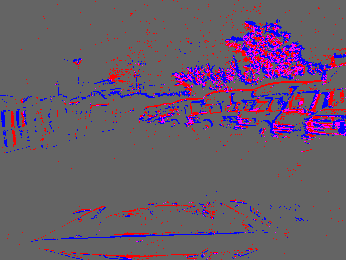
\includegraphics[width=0.31\linewidth]{mainmatter/figures/5_depth_transf/mvsec_cmp/data_and_gt/evts002965_lightgray_fixed.png} &
    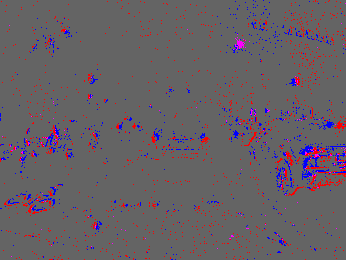
\includegraphics[width=0.31\linewidth]{mainmatter/figures/5_depth_transf/mvsec_cmp/data_and_gt/evts007350_lightgray_fixed.png} &
    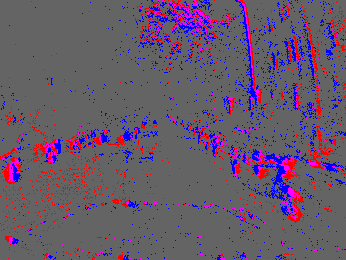
\includegraphics[width=0.31\linewidth]{mainmatter/figures/5_depth_transf/mvsec_cmp/data_and_gt/evts013112_lightgray_fixed.png} \\
    \raisebox{1.7cm}[0pt][0pt]{\rotatebox[origin=c]{90}{LiDAR proj.}} &
    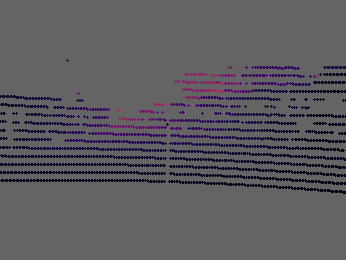
\includegraphics[width=0.31\linewidth]{mainmatter/figures/5_depth_transf/mvsec_cmp/data_and_gt/lidar002965_big_lightgray_fixed.png} &
    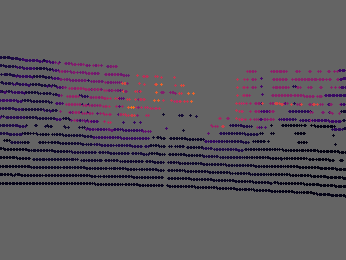
\includegraphics[width=0.31\linewidth]{mainmatter/figures/5_depth_transf/mvsec_cmp/data_and_gt/lidar007350_big_lightgray_fixed.png} &
    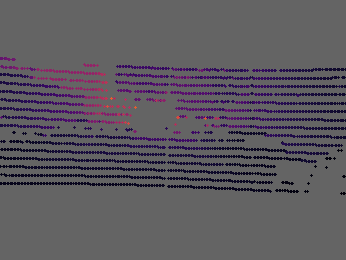
\includegraphics[width=0.31\linewidth]{mainmatter/figures/5_depth_transf/mvsec_cmp/data_and_gt/lidar013112_big_lightgray_fixed.png} \\
    \raisebox{1.7cm}[0pt][0pt]{\rotatebox[origin=c]{90}{Ground truth}} &
    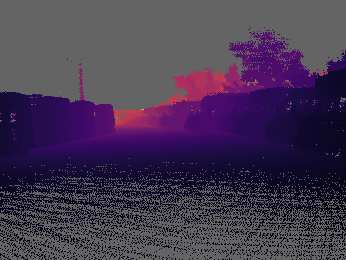
\includegraphics[width=0.31\linewidth]{mainmatter/figures/5_depth_transf/mvsec_cmp/data_and_gt/gtbf002965_lightgray_fixed.png} &
    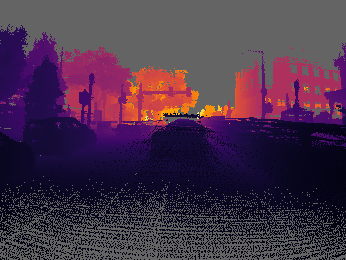
\includegraphics[width=0.31\linewidth]{mainmatter/figures/5_depth_transf/mvsec_cmp/data_and_gt/gtbf007350_lightgray_fixed.png} &
    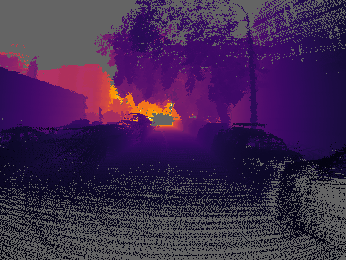
\includegraphics[width=0.31\linewidth]{mainmatter/figures/5_depth_transf/mvsec_cmp/data_and_gt/gtbf013112_lightgray_fixed.png} \\
    \raisebox{1.7cm}[0pt][0pt]{\rotatebox[origin=c]{90}{Cui \textit{et al.}~\cite{Cui2022DenseDE}}} &
    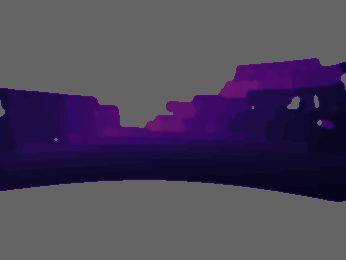
\includegraphics[width=0.31\linewidth]{mainmatter/figures/5_depth_transf/mvsec_cmp/cui_et_al/002965_pred_cvt_cropped_lightgray_fixed.png} &
    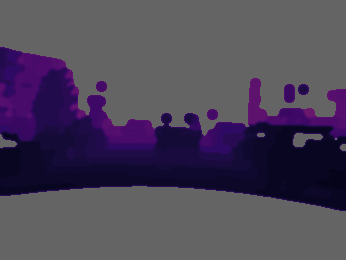
\includegraphics[width=0.31\linewidth]{mainmatter/figures/5_depth_transf/mvsec_cmp/cui_et_al/007350_pred_cvt_cropped_lightgray_fixed.png} &
    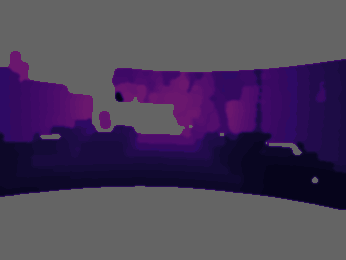
\includegraphics[width=0.31\linewidth]{mainmatter/figures/5_depth_transf/mvsec_cmp/cui_et_al/013112_pred_cvt_lightgray_fixed.png} \\
    \raisebox{1.7cm}[0pt][0pt]{\rotatebox[origin=c]{90}{ALED\textsubscript{SL\(\rightarrow\)MV}}} &
    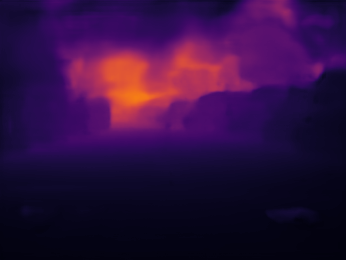
\includegraphics[width=0.31\linewidth]{mainmatter/figures/5_depth_transf/mvsec_cmp/aled/prev002965.png} &
    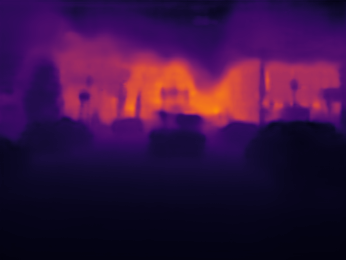
\includegraphics[width=0.31\linewidth]{mainmatter/figures/5_depth_transf/mvsec_cmp/aled/prev007350.png} &
    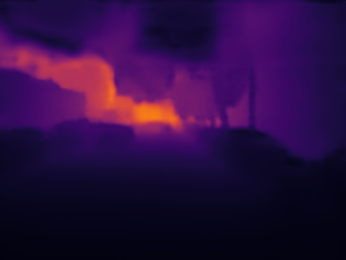
\includegraphics[width=0.31\linewidth]{mainmatter/figures/5_depth_transf/mvsec_cmp/aled/prev013112.png} \\
    \raisebox{1.7cm}[0pt][0pt]{\rotatebox[origin=c]{90}{DELTA\textsubscript{SL\(\rightarrow\)MV}}} &
    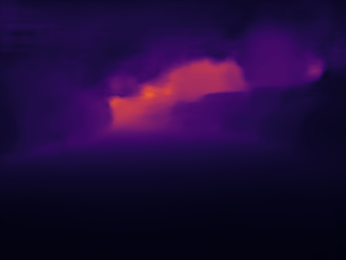
\includegraphics[width=0.31\linewidth]{mainmatter/figures/5_depth_transf/mvsec_cmp/delta/predbf002965.png} &
    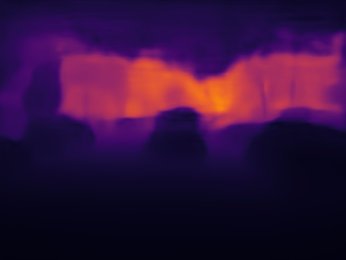
\includegraphics[width=0.31\linewidth]{mainmatter/figures/5_depth_transf/mvsec_cmp/delta/predbf007350.png} &
    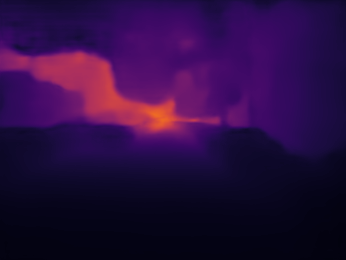
\includegraphics[width=0.31\linewidth]{mainmatter/figures/5_depth_transf/mvsec_cmp/delta/predbf013112.png}
  \end{tabular}
  \cprotect\caption{Qualitative results on the MVSEC dataset. From top to bottom: events; LiDAR projection (with size of points increased for a better visibility); ground truth; results from Cui \textit{et al.}~\cite{Cui2022DenseDE}; results from ALED\textsubscript{SL\(\rightarrow\)MV}; results from DELTA\textsubscript{SL\(\rightarrow\)MV}. Sequences shown, from left to right: \verb|outdoor_day_1|; \verb|outdoor_night_1|; \verb|outdoor_night_2|.}\label{fig:delta:cmp_mvsec}
\end{figure}

If the reader is interested, more qualitative results are given in \cref{sec:appendix:delta:visual_results_mvsec}, and results in video format are available through the link given at the very beginning of this chapter (\cpageref{sec:delta}).

\subsection{Results on the M3ED Dataset}
Like the evaluation on the MVSEC dataset, we follow two distinct strategies when evaluating on the M3ED dataset:
\begin{itemize}
  \item we only train it on M3ED, noted as DELTA\textsubscript{M3}, and
  \item we reuse the weights trained on the \acrshort{sled} dataset, DELTA\textsubscript{SL}, and finetune them on the M3ED dataset: we denote it DELTA\textsubscript{SL\(\rightarrow\)M3}.
\end{itemize}
Both the results of DELTA\textsubscript{M3} and of DELTA\textsubscript{SL\(\rightarrow\)M3} are given in \cref{tab:delta:results_m3ed}.

\begin{table}[ht]
  \centering
  \scalebox{0.75}{
    \begin{tabular}{@{}cccc@{}}
      \toprule
      Recording & Cutoff & DELTA\textsubscript{M3} & DELTA\textsubscript{SL\(\rightarrow\)M3} \\
      \midrule
      \multirow{5}{*}{\Verb|city_hall_day|} & 10m & \textbf{0.30} & 0.58 \\
      & 20m & \textbf{0.45} & 0.71 \\
      & 30m & \textbf{0.60} & 0.85 \\
      & 60m & \textbf{0.92} & 1.07 \\
      & 120m & \textbf{1.02} & 1.19 \\
      \midrule
      \multirow{5}{*}{\Verb|city_hall_night|} & 10m & \textbf{0.26} & 0.55 \\
      & 20m & \textbf{0.39} & 0.67 \\
      & 30m & \textbf{0.49} & 0.79 \\
      & 60m & \textbf{0.69} & 1.02 \\
      & 120m & \textbf{0.81} & 1.21 \\
      \bottomrule
    \end{tabular}
  }
  \caption{Absolute depth errors (in meters) on the M3ED dataset for various cutoff depth distances (for the ``before'' depth maps \(D_\text{bf}\)).}\label{tab:delta:results_m3ed}
\end{table}

Again, the errors remain very low on both sequences, with the error at the maximum cutoff distance being close to or under 1m. Yet, results here differ from those on the \acrshort{sled} and MVSEC datasets, as better errors are obtained when training directly on the M3ED dataset than when pre-training on the \acrshort{sled} dataset. This apparent discrepancy can be explained when observing the visual results given in \cref{fig:delta:cmp_m3ed}. As shown, the ground truth depth maps of the M3ED dataset are very sparse, and due to the process used for building them, ground truth values are concentrated in the center of the objects, with very few values at their edges. As such, by being only trained on this dataset, DELTA\textsubscript{M3} outputs good numerical errors, but poor-looking depth maps with large blobs and a scanline effect following the outline of LiDAR points projection, making the identification of objects difficult. On the contrary, the pre-training on the \acrshort{sled} dataset allows DELTA\textsubscript{SL\(\rightarrow\)M3} to output depth maps where objects appear more clearly (for instance, the lamp post in the top-left part of \cref{fig:delta:cmp_m3ed}). However, by doing so, the output depth maps are more rough. Another element which could explain why the finetuning is difficult is that network inputs when using M3ED are intrinsically different from those of \acrshort{sled}, with events being accumulated over 100ms instead of 50ms (see \cref{sec:delta:eval:impl_detail:data_repres}), and with the LiDAR data covering the whole vertical range of the image.

\begin{figure}
  \centering
  \setlength\tabcolsep{1pt}
  \renewcommand{\arraystretch}{0.5}
  \begin{tabular}{@{}ccc@{}}
    \raisebox{2cm}[0pt][0pt]{\rotatebox[origin=c]{90}{Events}} &
    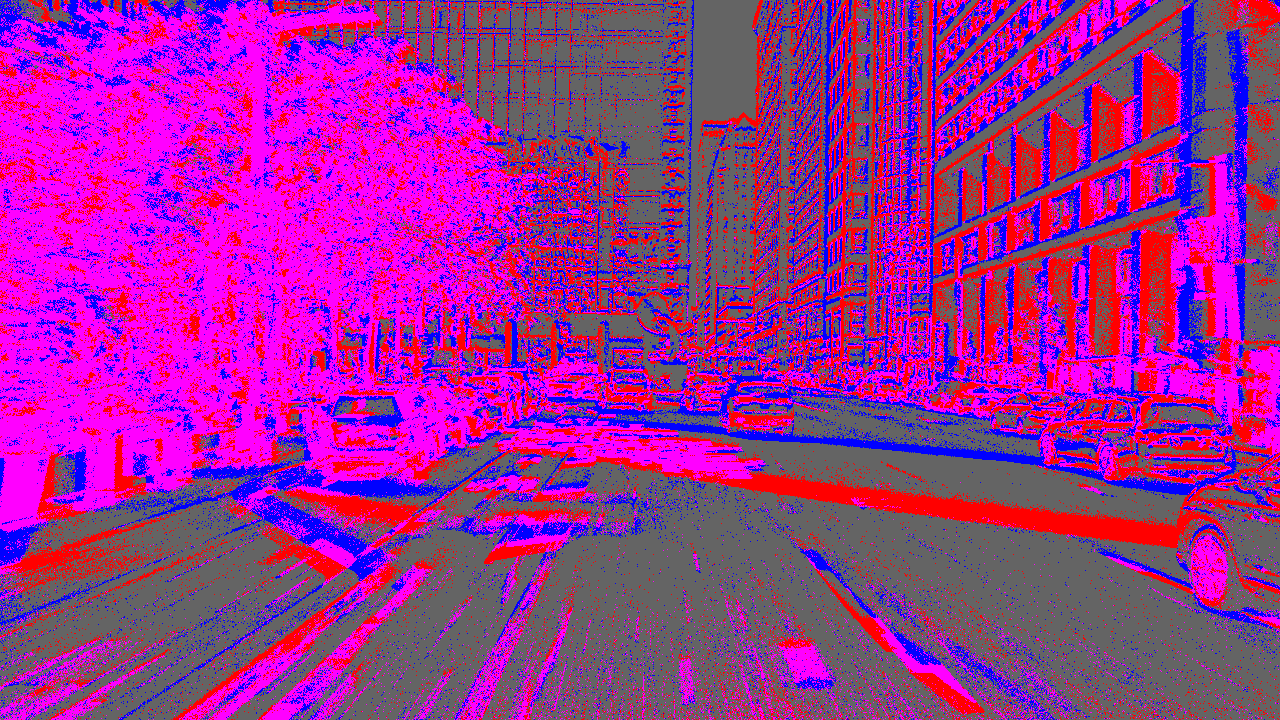
\includegraphics[width=0.475\linewidth]{mainmatter/figures/5_depth_transf/m3ed_cmp/evts000198_lightgray_fixed.png} &
    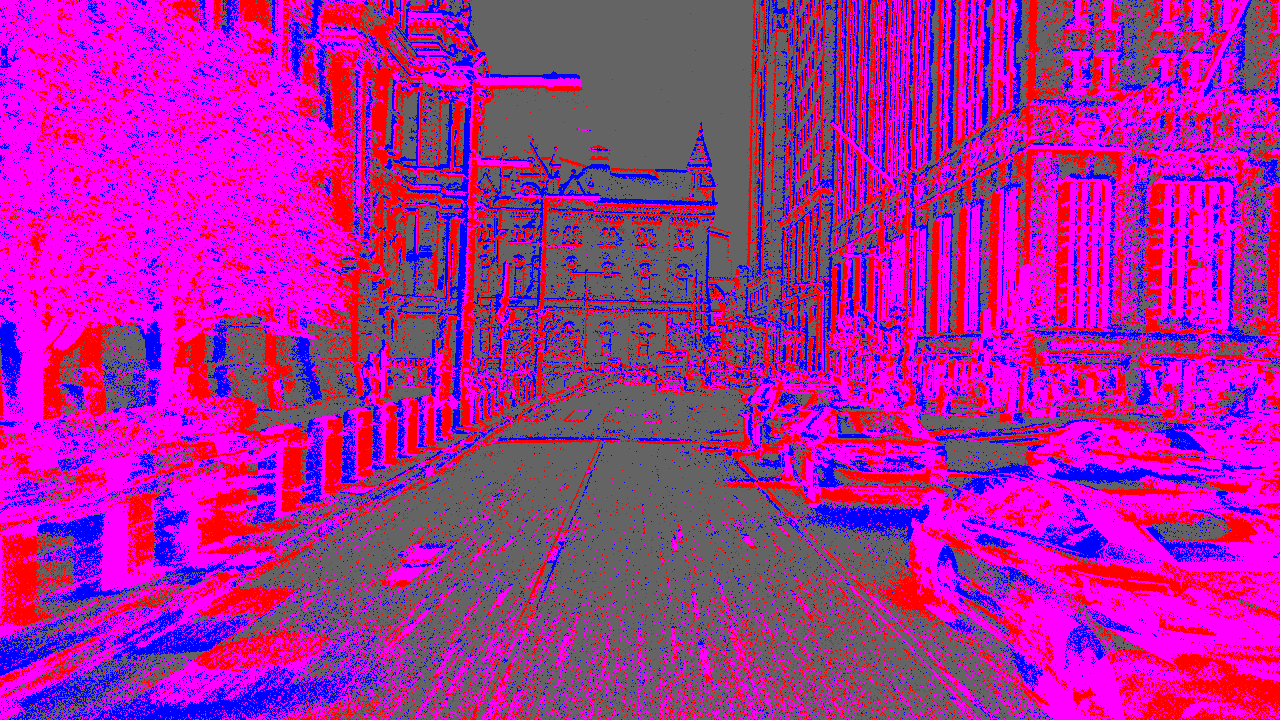
\includegraphics[width=0.475\linewidth]{mainmatter/figures/5_depth_transf/m3ed_cmp/evts000518_lightgray_fixed.png} \\
    \raisebox{2cm}[0pt][0pt]{\rotatebox[origin=c]{90}{LiDAR proj.}} &
    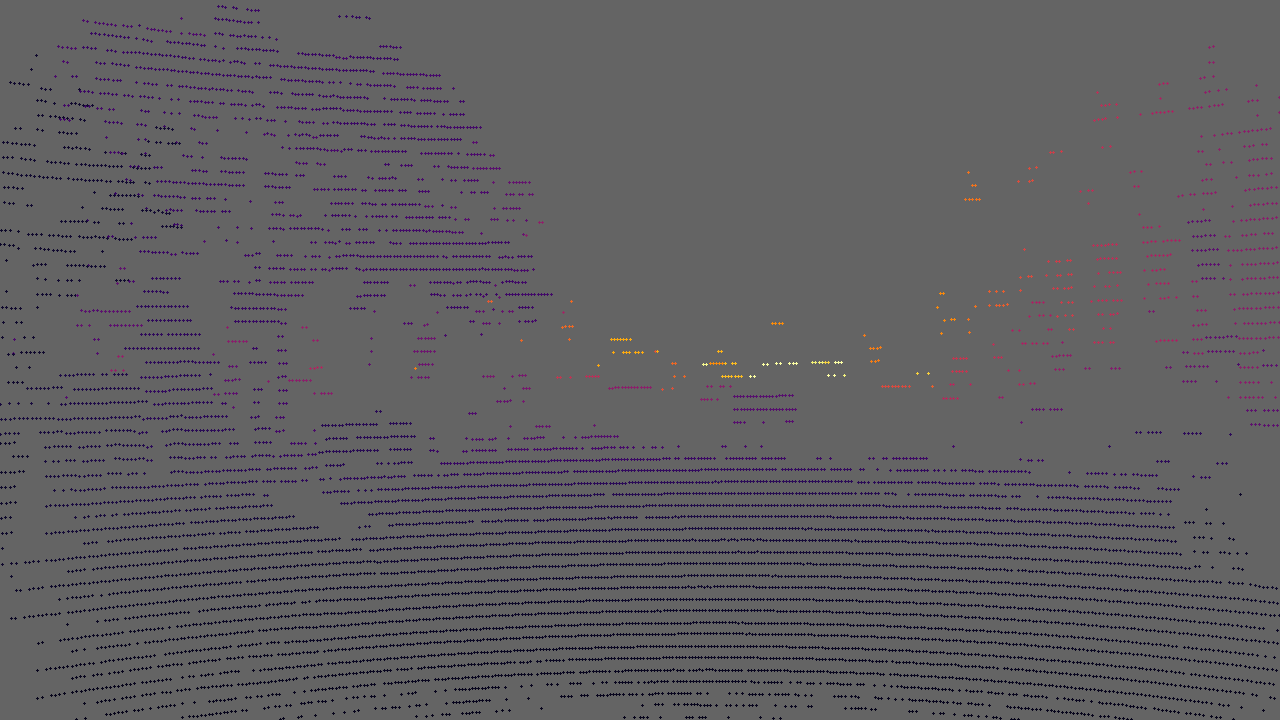
\includegraphics[width=0.475\linewidth]{mainmatter/figures/5_depth_transf/m3ed_cmp/lidar000198_lightgray_fixed.png} &
    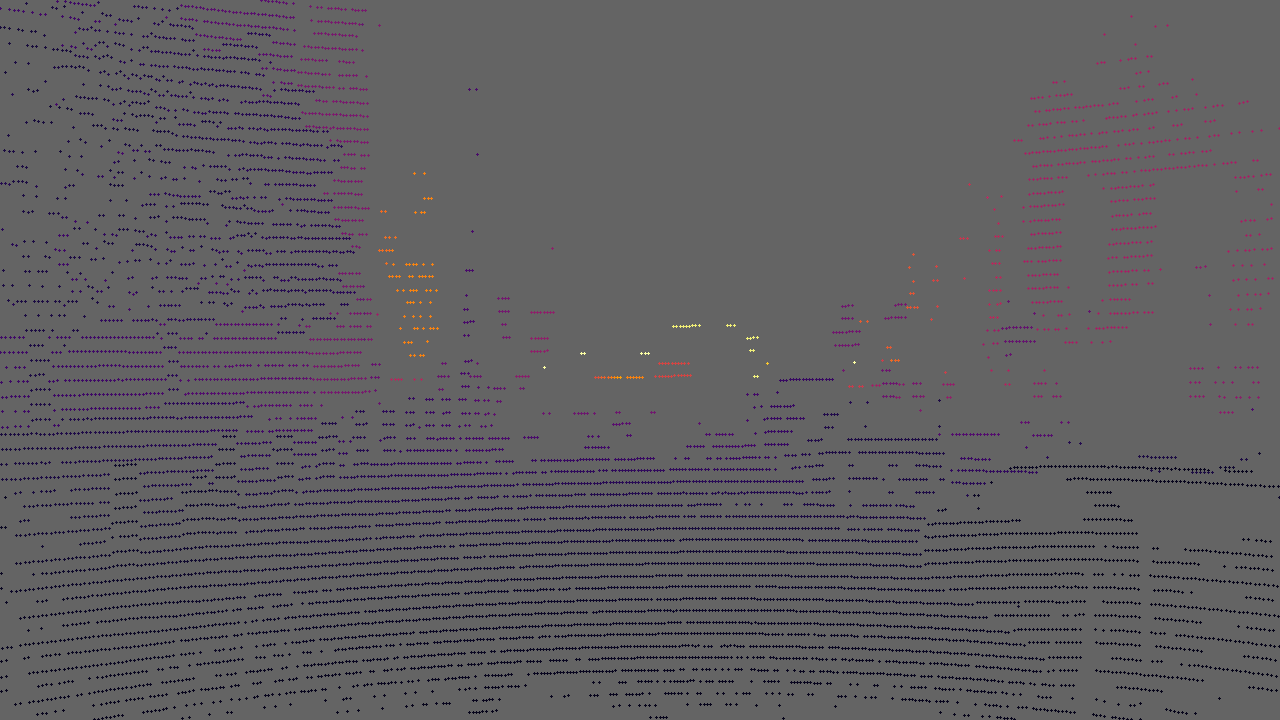
\includegraphics[width=0.475\linewidth]{mainmatter/figures/5_depth_transf/m3ed_cmp/lidar000518_lightgray_fixed.png} \\
    \raisebox{2cm}[0pt][0pt]{\rotatebox[origin=c]{90}{Ground truth}} &
    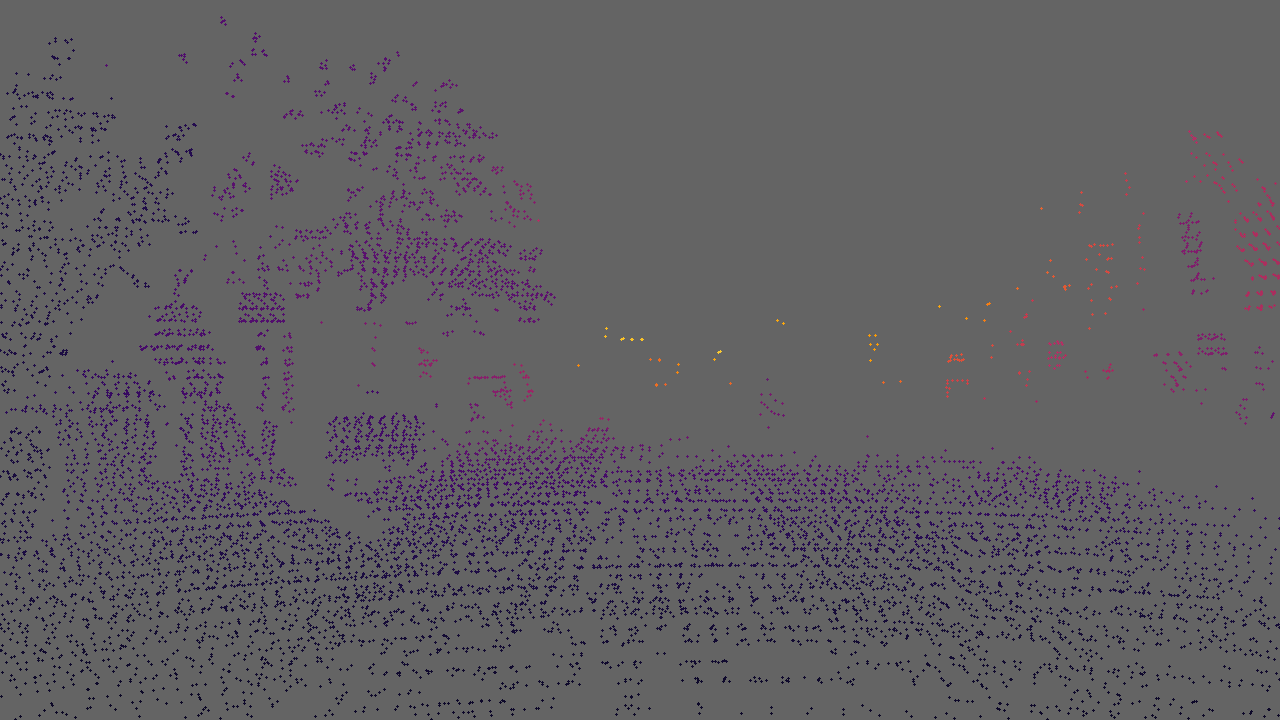
\includegraphics[width=0.475\linewidth]{mainmatter/figures/5_depth_transf/m3ed_cmp/gtbf000198_lightgray_fixed.png} &
    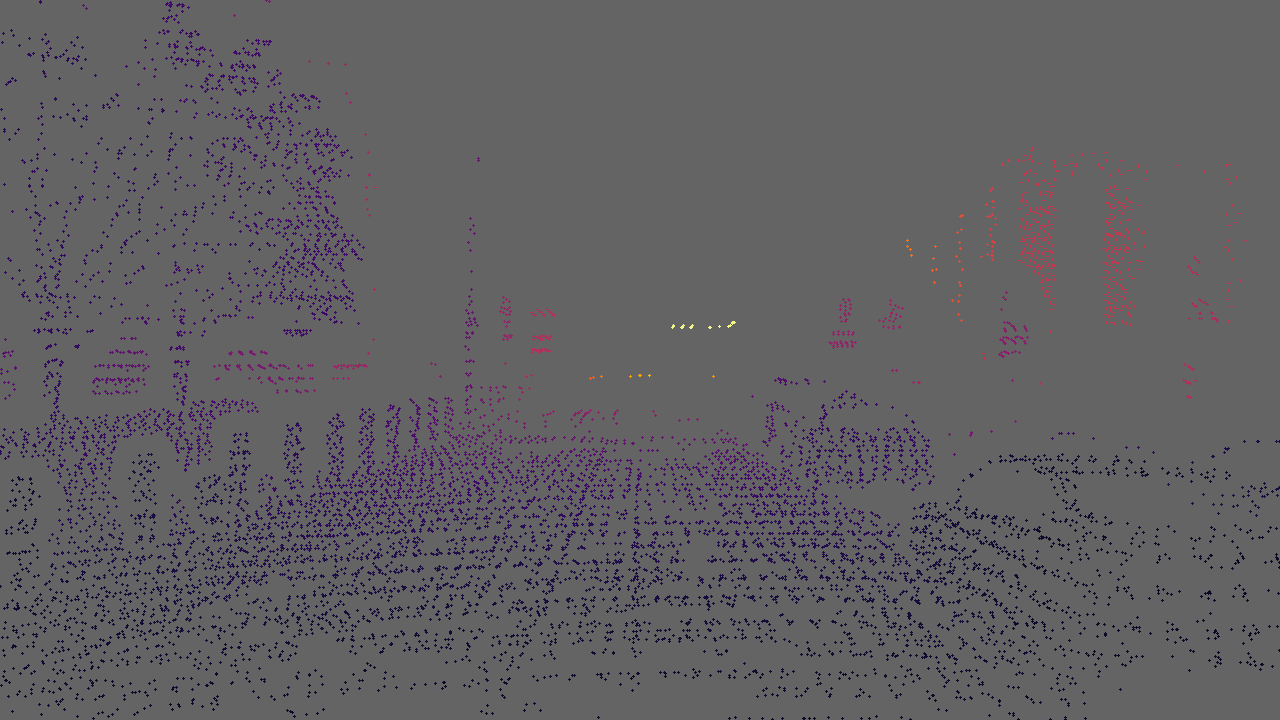
\includegraphics[width=0.475\linewidth]{mainmatter/figures/5_depth_transf/m3ed_cmp/gtbf000518_lightgray_fixed.png} \\
    \raisebox{2cm}[0pt][0pt]{\rotatebox[origin=c]{90}{DELTA\textsubscript{M3}}} &
    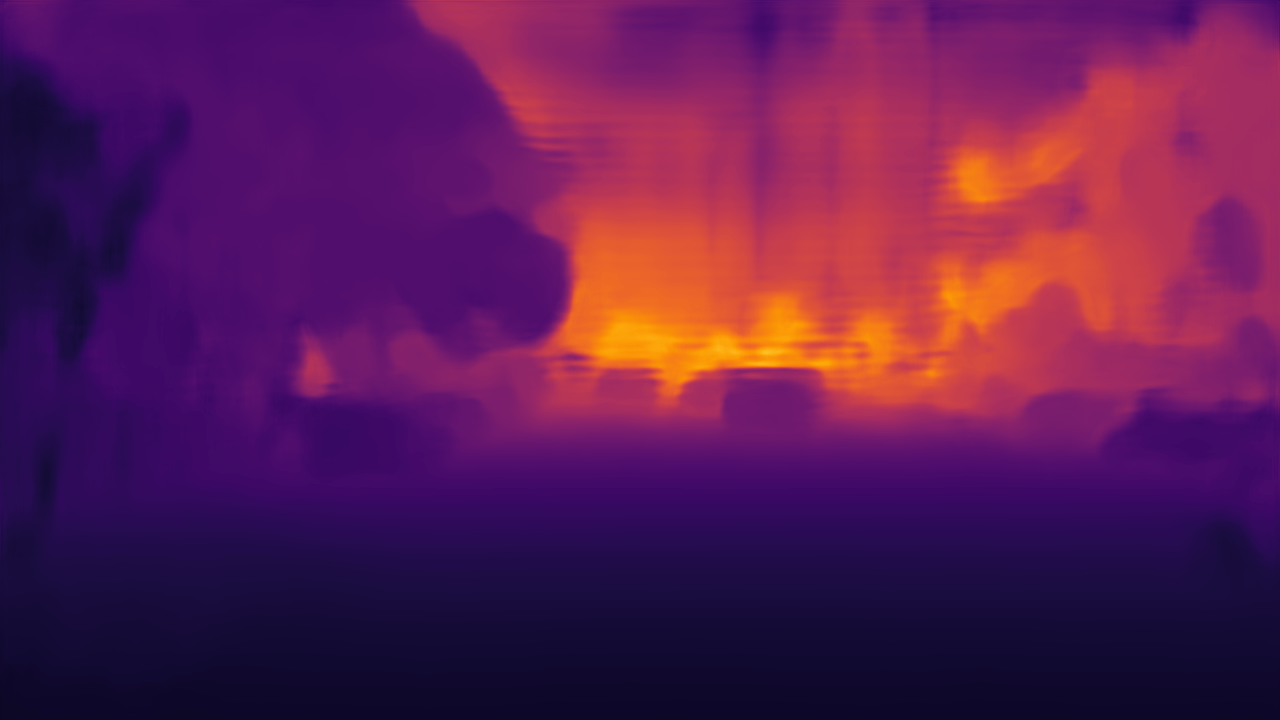
\includegraphics[width=0.475\linewidth]{mainmatter/figures/5_depth_transf/m3ed_cmp/predbf000198_M3.png} &
    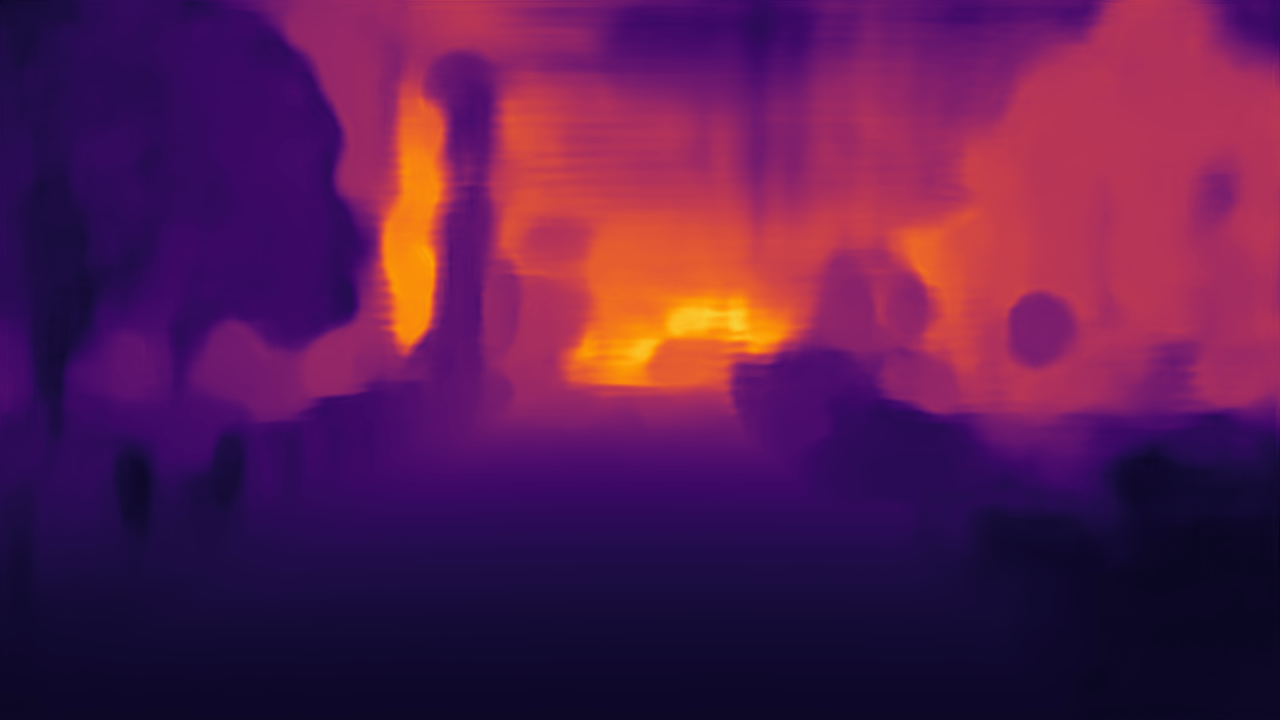
\includegraphics[width=0.475\linewidth]{mainmatter/figures/5_depth_transf/m3ed_cmp/predbf000518_M3.png} \\
    \raisebox{2cm}[0pt][0pt]{\rotatebox[origin=c]{90}{DELTA\textsubscript{SL\(\rightarrow\)M3}}} &
    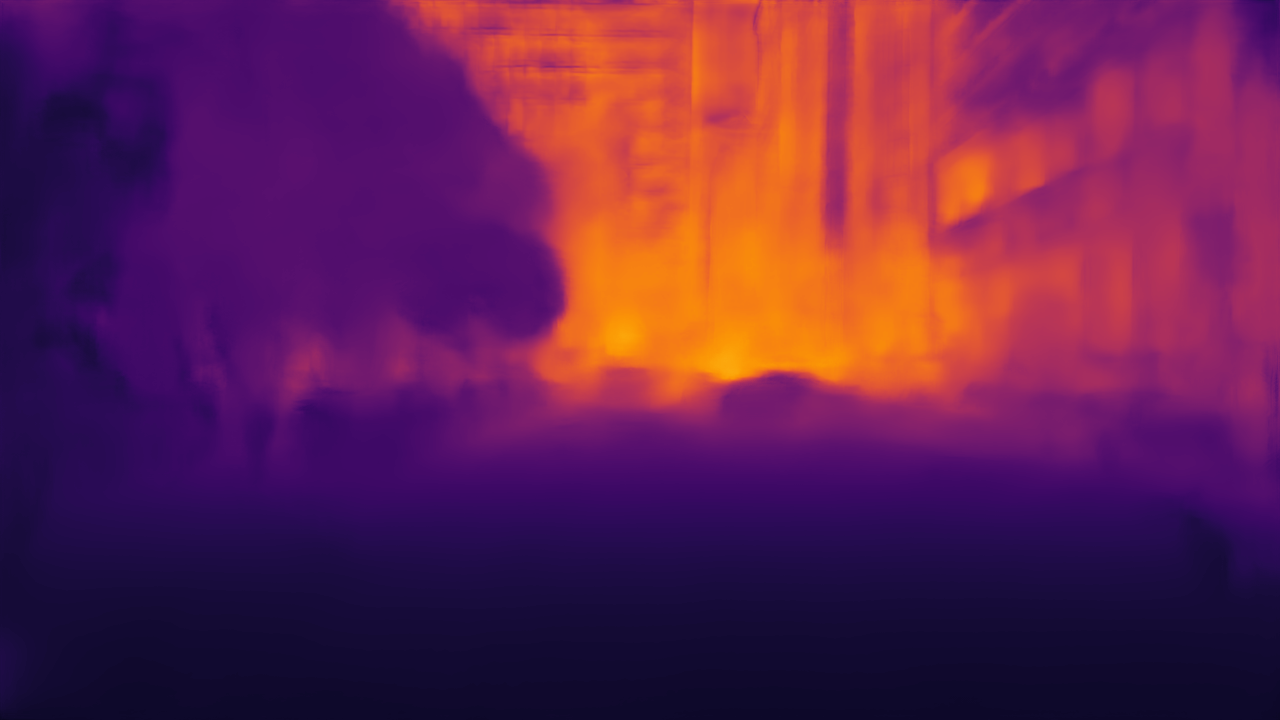
\includegraphics[width=0.475\linewidth]{mainmatter/figures/5_depth_transf/m3ed_cmp/predbf000198_SL_M3.png} &
    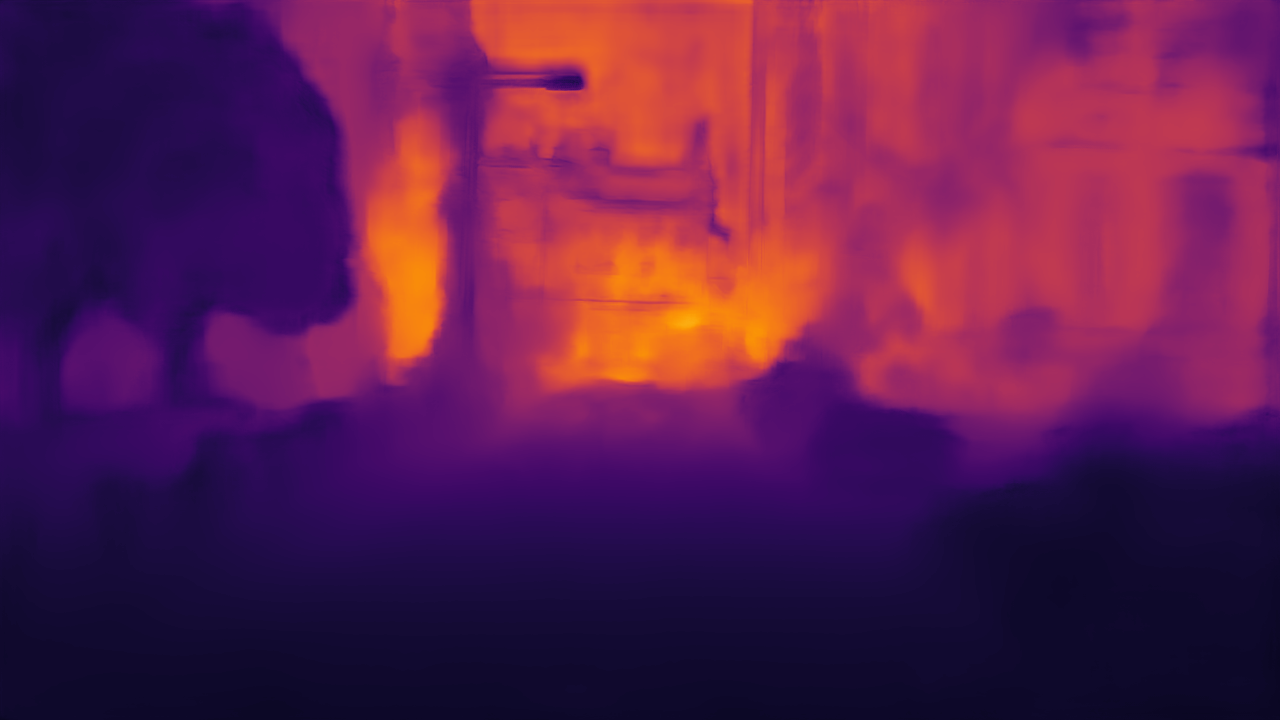
\includegraphics[width=0.475\linewidth]{mainmatter/figures/5_depth_transf/m3ed_cmp/predbf000518_SL_M3.png}
  \end{tabular}
  \cprotect\caption{Qualitative results for the \verb|city_hall_day| sequence from M3ED. The size of points for both the LiDAR projection and the ground truth was increased for a better visibility. Zoom on numerical version is required to see the scanline effect on DELTA\textsubscript{M3}.}\label{fig:delta:cmp_m3ed}
\end{figure}

If the reader is interested, more qualitative results are given in \cref{sec:appendix:delta:visual_results_m3ed}, and results in video format are available through the link given at the very beginning of this chapter (\cpageref{sec:delta}).

\subsection{Ablation Study}\label{sec:delta:eval:ablation}

\begin{figure}
  \centering

  % Defining the colors that will be used
  \definecolor{color_l}{RGB}{204,187,68}
  \definecolor{color_e}{RGB}{238,102,119}
  \definecolor{color_d}{RGB}{34,136,51}
  \definecolor{color_ca}{RGB}{68,119,170}
  \definecolor{color_sa}{RGB}{102,204,238}
  \definecolor{color_gru}{RGB}{187,187,187}
  \definecolor{color_sk}{RGB}{140,140,140}
  \definecolor{color_skd}{RGB}{170,51,119}

  \scalebox{0.55}{
    \shorthandoff{:!}
    \begin{tikzpicture}[every node/.style={inner sep=0.001,outer sep=0.001,font=\normalsize}]
      % Changing the font
      \fontfamily{cmss}\selectfont

      % Helping grid
      %\draw[help lines] (0,0) grid (22,-16);

      % LiDAR encoding
      \node[] (L) at (0,0) {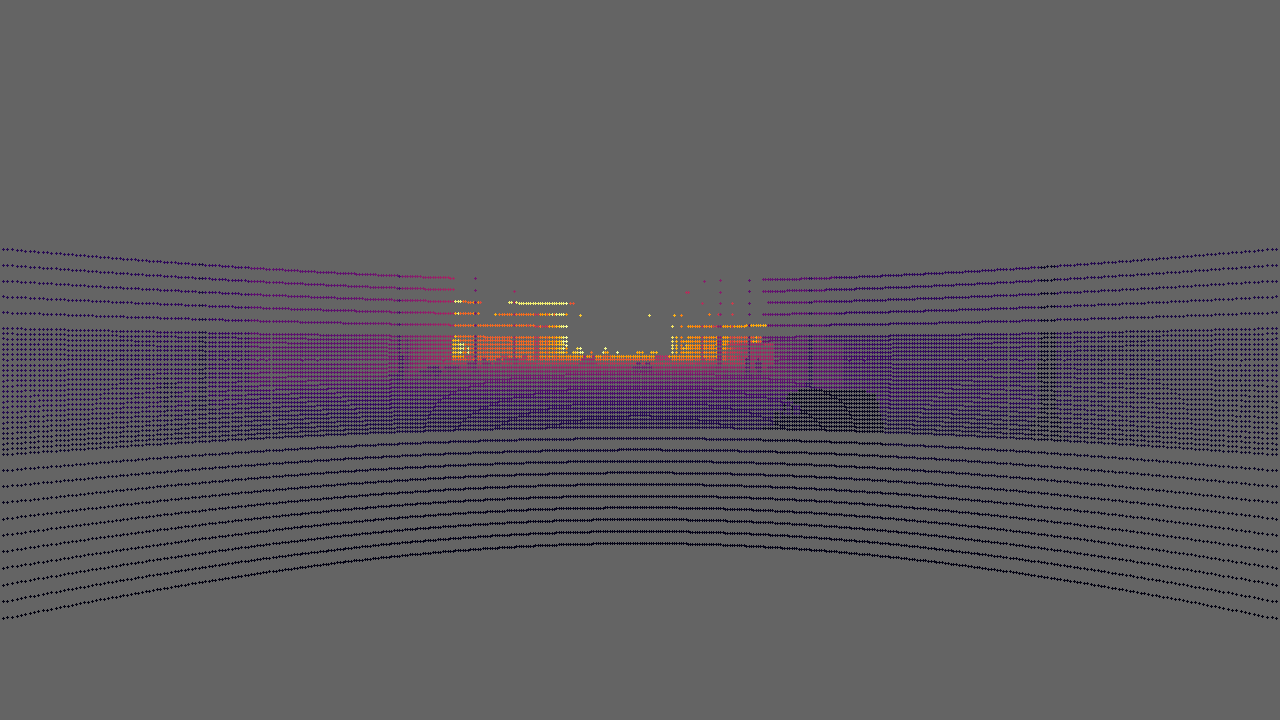
\includegraphics[height=2cm,cfbox=color_l 0.05cm 0pt]{mainmatter/figures/5_depth_transf/network/lidar005158_lightgray_fixed.png}};
      \node[above=0.1cm of L] (Ll) {\normalsize Input LiDAR};

      \node[draw, trapezium, minimum width=1.25cm, on grid, right=4.5cm of L, opacity=0.0] (tmplh) {};
      \node[draw, trapezium, fill=color_l, minimum width=1.25cm, rotate around={-90:(tmplh.center)}] (LH) at (tmplh) {};

      \node[draw, circle, minimum width=0.625cm, right=0.5cm of tmplh] (LP) {\Large +};

      \node[draw, fill=color_sa, rounded corners, minimum width=1cm, minimum height=1cm, right=2cm of LP] (LSA1) {SA};

      \node[draw, fill=color_sa, rounded corners, minimum width=1cm, minimum height=1cm, right=1.5cm of LSA1] (LSA2) {SA};

      % Events encoding + propagation memory
      \node[below=2.9cm of L] (E) {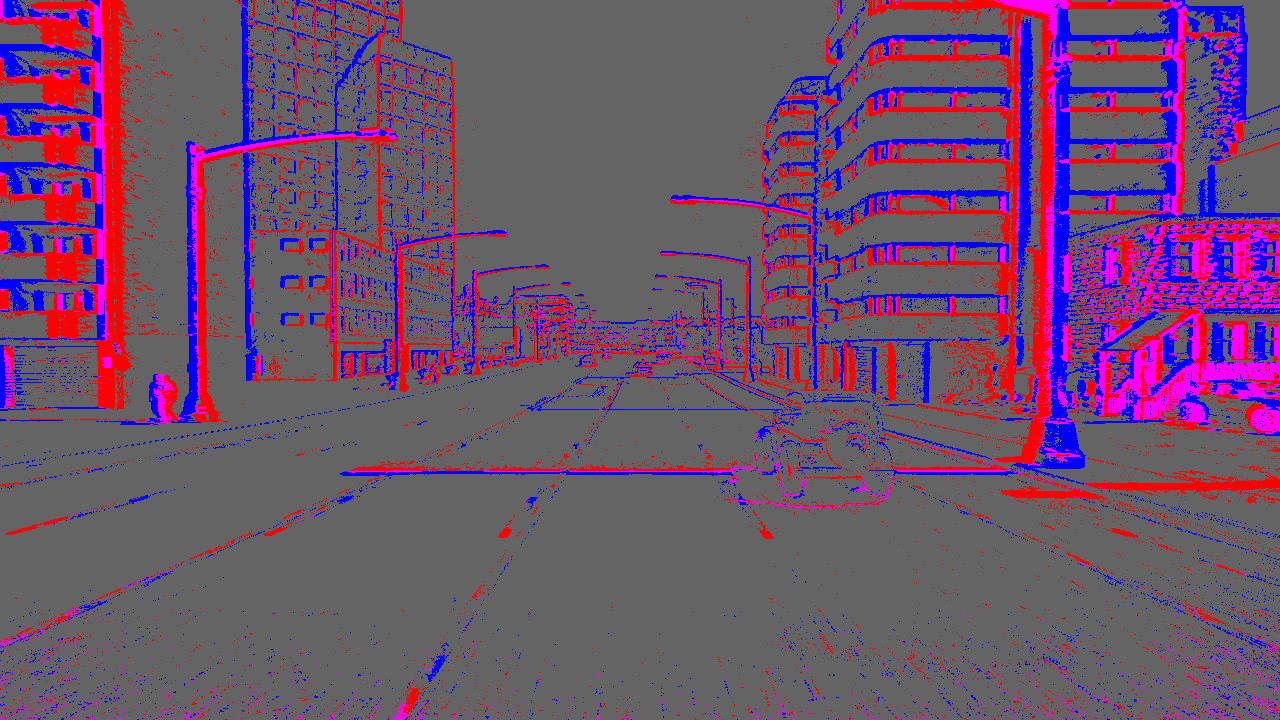
\includegraphics[height=2cm,cfbox=color_e 0.05cm 0pt]{mainmatter/figures/5_depth_transf/network/evts005158_lightgray_fixed.png}};
      \node[above=0.1cm of E] (El) {\normalsize Input Events};

      \node[draw, trapezium, minimum width=1.25cm, on grid, right=4.5cm of E, opacity=0.0] (tmpeh) {};
      \node[draw, trapezium, fill=color_e, minimum width=1.25cm, rotate around={-90:(tmpeh.center)}] (EH) at (tmpeh) {};

      \node[draw, circle, minimum width=0.625cm, right=0.5cm of tmpeh] (EP) {\Large +};

      \node[draw, fill=color_sa, rounded corners, minimum width=1cm, minimum height=1cm, right=2cm of EP] (ESA1) {SA};

      \node[draw, fill=color_sa, rounded corners, minimum width=1cm, minimum height=1cm, right=1.5cm of ESA1] (ESA2) {SA};

      % Positional encoding
      \node[draw, circle, minimum width=1cm, minimum height=1cm, between=LP and EP] (PE) {};
      \draw[thick] ($(PE)+(-0.5cm,0)$) sin ($(PE)+(-0.25cm,0.3cm)$) cos (PE) sin ($(PE)+(0.25cm,-0.3cm)$) cos ($(PE)+(0.5cm,0)$);

      % Central memory update
      \node[draw, fill=color_ca, rounded corners, minimum width=1cm, minimum height=1cm, below right=1.5cm and 0.75cm of LSA2] (MCA) {CA\textsubscript{F}};

      \node[draw, fill=color_gru, rounded corners, minimum width=1cm, minimum height=1cm, right=0.75cm of MCA] (MGRU) {GRU};

      \node[draw, minimum width=1cm, minimum height=1cm, right=0.75cm of MGRU, align=center] (M) {Cent.\\mem.};

      % Decoding
      \node[draw, fill=color_sa, rounded corners, minimum width=1cm, minimum height=1cm, on grid, below=3.5cm of ESA2] (DSA2) {SA};

      \node[draw, fill=color_sa, rounded corners, minimum width=1cm, minimum height=1cm, left=1.5cm of DSA2] (DSA1) {SA};

      \node[draw, trapezium, minimum width=1.25cm, left=3.13cm of DSA1, opacity=0.0] (tmpdh) {};
      \node[draw, trapezium, fill=color_d, minimum width=1.25cm, rotate around={-90:(tmpdh.center)}] (DH) at (tmpdh) {};

      \node[on grid, left=4.5cm of tmpdh] (D) {
        \begin{tikzpicture}
          \node[on grid] (Daf) {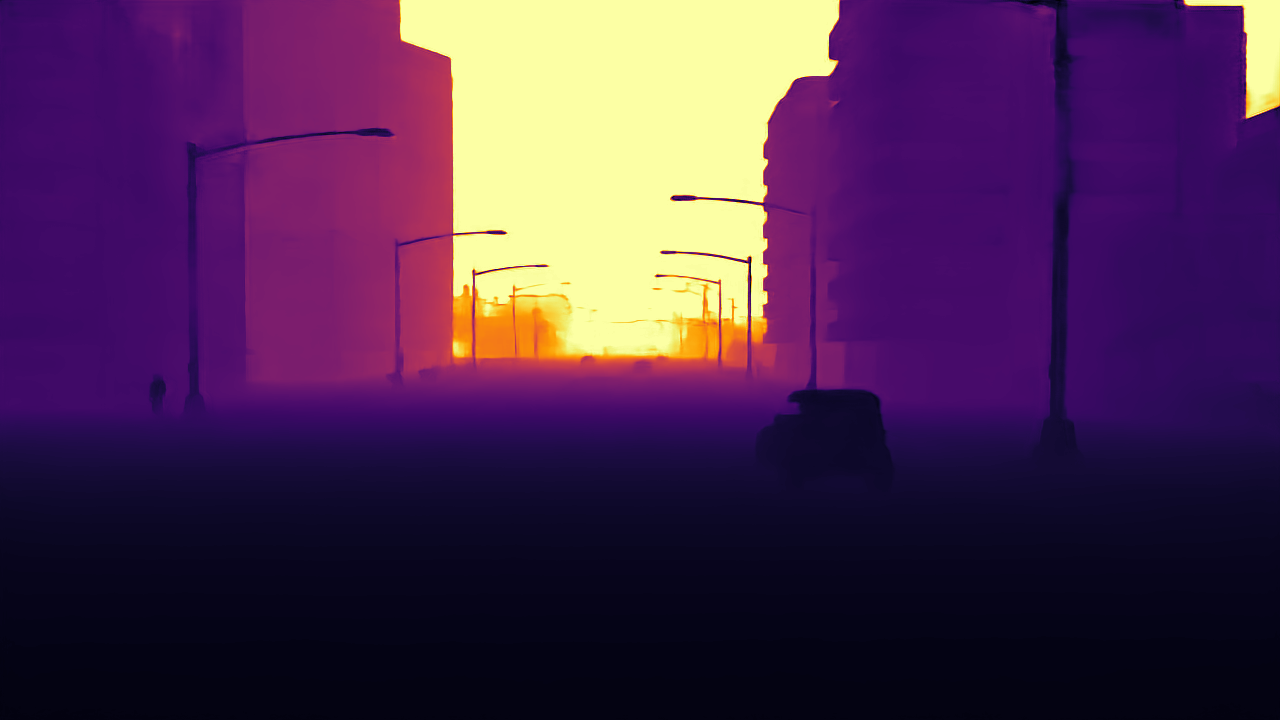
\includegraphics[height=1.85cm,cfbox=color_d 0.05cm 0pt]{mainmatter/figures/5_depth_transf/network/predaf005158.png}};
          \node[on grid, below left=0.25cm and 0.25cm of Daf] (Dbf) {\includegraphics[height=1.85cm,cfbox=color_d 0.05cm 0pt]{mainmatter/figures/5_depth_transf/network/predbf005158.png}};
        \end{tikzpicture}
      };
      \node[above=0.1cm of D] (Dl) {\normalsize Output Depth Maps};

      % Skip connections (SA)
      \node[draw, circle, color_sk, minimum width=0.625cm, below left=1.6875cm and 0.75cm of LSA1] (SP1a) {\Large +};
      \node[draw, circle, color_sk, minimum width=0.625cm, below left=1.6875cm and 0.75cm of LSA2] (SP2a) {\Large +};
      \node[draw, circle, color_sk, minimum width=0.625cm, left=0.25cm of DSA1] (SP1b) {\Large +};
      \node[draw, circle, color_sk, minimum width=0.625cm, left=0.25cm of DSA2] (SP2b) {\Large +};

      % Paths
      \draw[dashed, color_sk, ->, >=latex, line width=0.5mm] (ESA1.west -| SP1a) -- (SP1a);
      \draw[dashed, color_sk, ->, >=latex, line width=0.5mm] (ESA2.west -| SP2a) -- (SP2a);
      \draw[dashed, color_sk, ->, >=latex, line width=0.5mm] (LSA1.west -| SP1a) -- (SP1a);
      \draw[dashed, color_sk, ->, >=latex, line width=0.5mm] (LSA1.west -| SP2a) -- (SP2a);
      \draw[dashed, color_sk, ->, >=latex, line width=0.5mm] (SP1a) -| (SP1b);
      \draw[dashed, color_sk, ->, >=latex, line width=0.5mm] (SP2a) -| (SP2b);
      \draw[dashdotted, color_skd, ->, >=latex, line width=0.5mm] (EH) -- (DH);

      \draw[->,>=latex, line width=0.5mm, color_l] (L) -- node [above=0.1cm, midway] (al) {(B, H, W, 1)} (LH);
      \draw[->,>=latex, line width=0.5mm, color_l] (LH) -- (LP);
      \draw[->,>=latex, line width=0.5mm, color_l] (LP) -- (LSA1);
      \draw[->,>=latex, line width=0.5mm, color_l] (LSA1) -- (LSA2);
      \draw[->,>=latex, line width=0.5mm, color_l] (LSA2) -| node [left=0.1cm, pos=0.95] (amkv) {\color{color_ca} \textbf{K/V}} (MCA);

      \draw[->,>=latex, line width=0.5mm, color_e] (E) -- node [above=0.1cm, midway] (ae) {(B, H, W, 4)} (EH);
      \draw[->,>=latex, line width=0.5mm, color_e] (EH) -- (EP);
      \draw[->,>=latex, line width=0.5mm, color_e] (EP) -- (ESA1);
      \draw[->,>=latex, line width=0.5mm, color_e] (ESA1) -- (ESA2);
      \draw[->,>=latex, line width=0.5mm, color_e] (ESA2) -| node [left=0.1cm, pos=0.935] (amq) {\color{color_ca} \textbf{Q}} (MCA);

      \draw[->,>=latex, line width=0.5mm] (PE) -- (LP);
      \draw[->,>=latex, line width=0.5mm] (PE) -- (EP);

      \draw[->,>=latex, line width=0.5mm] (MCA) -- (MGRU);
      \draw[->,>=latex, line width=0.5mm] ([yshift=0.2cm] M.west) -- ([yshift=0.2cm] MGRU.east);
      \draw[->,>=latex, line width=0.5mm] ([yshift=-0.2cm] MGRU.east) -- ([yshift=-0.2cm] M.west);

      \draw[->,>=latex, line width=0.5mm, color_d] (M) |- (DSA2);
      \draw[->,>=latex, line width=0.5mm, color_d] (DSA2) -- (SP2b);
      \draw[->,>=latex, line width=0.5mm, color_d] (SP2b) -- (DSA1);
      \draw[->,>=latex, line width=0.5mm, color_d] (DSA1) -- (SP1b);
      \draw[->,>=latex, line width=0.5mm, color_d] (SP1b) -- (DH);
      \draw[->,>=latex, line width=0.5mm, color_d] (DH) -- node [above=0.1cm, midway] (ad) {(B, H, W, 2)} (D);
    \end{tikzpicture}
    \shorthandon{:!}
  }
  \caption{The alternative architecture without propagation memory, DELTA\textsuperscript{NPM}.}\label{fig:delta:network_alt_npm}

  \vspace{10mm}

  \scalebox{0.55}{
    \shorthandoff{:!}
    \begin{tikzpicture}[every node/.style={inner sep=0.001,outer sep=0.001,font=\normalsize}]
      % Changing the font
      \fontfamily{cmss}\selectfont

      % Helping grid
      %\draw[help lines] (0,0) grid (22,-16);

      % LiDAR encoding
      \node[] (L) at (0,0) {\includegraphics[height=2cm,cfbox=color_l 0.05cm 0pt]{mainmatter/figures/5_depth_transf/network/lidar005158_lightgray_fixed.png}};
      \node[above=0.1cm of L] (Ll) {\normalsize Input LiDAR};

      \node[draw, trapezium, minimum width=1.25cm, on grid, right=4.5cm of L, opacity=0.0] (tmplh) {};
      \node[draw, trapezium, fill=color_l, minimum width=1.25cm, rotate around={-90:(tmplh.center)}] (LH) at (tmplh) {};

      \node[draw, circle, minimum width=0.625cm, right=0.5cm of tmplh] (LP) {\Large +};

      \node[draw, fill=color_ca, rounded corners, minimum width=1cm, minimum height=1cm, right=2.25cm of LP] (LCA) {CA\textsubscript{P2}};

      \node[draw, fill=color_sa, rounded corners, minimum width=1cm, minimum height=1cm, right=3.25cm of LCA] (LSA1) {SA};

      \node[draw, fill=color_sa, rounded corners, minimum width=1cm, minimum height=1cm, right=1.5cm of LSA1] (LSA2) {SA};

      % Events encoding + propagation memory
      \node[below=2.9cm of L] (E) {\includegraphics[height=2cm,cfbox=color_e 0.05cm 0pt]{mainmatter/figures/5_depth_transf/network/evts005158_lightgray_fixed.png}};
      \node[above=0.1cm of E] (El) {\normalsize Input Events};

      \node[draw, trapezium, minimum width=1.25cm, on grid, right=4.5cm of E, opacity=0.0] (tmpeh) {};
      \node[draw, trapezium, fill=color_e, minimum width=1.25cm, rotate around={-90:(tmpeh.center)}] (EH) at (tmpeh) {};

      \node[draw, circle, minimum width=0.625cm, right=0.5cm of tmpeh] (EP) {\Large +};

      \node[draw, fill=color_ca, rounded corners, minimum width=1cm, minimum height=1cm, below=2.6667cm of LCA] (PCA) {CA\textsubscript{P1}};

      \node[draw, minimum width=1cm, minimum height=1cm, above=0.8cm of PCA, align=center] (P) {Prop.\\mem.};

      \node[draw, fill=color_sa, rounded corners, minimum width=1cm, minimum height=1cm, below right=0.3333cm and 3.25cm of PCA] (ESA1) {SA};

      \node[draw, fill=color_sa, rounded corners, minimum width=1cm, minimum height=1cm, right=1.5cm of ESA1] (ESA2) {SA};

      % Positional encoding
      \node[draw, circle, minimum width=1cm, minimum height=1cm, between=LP and EP] (PE) {};
      \draw[thick] ($(PE)+(-0.5cm,0)$) sin ($(PE)+(-0.25cm,0.3cm)$) cos (PE) sin ($(PE)+(0.25cm,-0.3cm)$) cos ($(PE)+(0.5cm,0)$);

      % Central memory update
      \node[draw, fill=color_ca, rounded corners, minimum width=1cm, minimum height=1cm, below right=1.5cm and 0.75cm of LSA2] (MCA) {CA\textsubscript{F}};

      % Decoding
      \node[draw, fill=color_sa, rounded corners, minimum width=1cm, minimum height=1cm, on grid, below=3.5cm of ESA2] (DSA2) {SA};

      \node[draw, fill=color_sa, rounded corners, minimum width=1cm, minimum height=1cm, left=1.5cm of DSA2] (DSA1) {SA};

      \node[draw, trapezium, minimum width=1.25cm, on grid, below=3.5cm of tmpeh, opacity=0.0] (tmpdh) {};
      \node[draw, trapezium, fill=color_d, minimum width=1.25cm, rotate around={-90:(tmpdh.center)}] (DH) at (tmpdh) {};

      \node[on grid, left=4.5cm of tmpdh] (D) {
        \begin{tikzpicture}
          \node[on grid] (Daf) {\includegraphics[height=1.85cm,cfbox=color_d 0.05cm 0pt]{mainmatter/figures/5_depth_transf/network/predaf005158.png}};
          \node[on grid, below left=0.25cm and 0.25cm of Daf] (Dbf) {\includegraphics[height=1.85cm,cfbox=color_d 0.05cm 0pt]{mainmatter/figures/5_depth_transf/network/predbf005158.png}};
        \end{tikzpicture}
      };
      \node[above=0.1cm of D] (Dl) {\normalsize Output Depth Maps};

      % Skip connections (SA)
      \node[draw, circle, color_sk, minimum width=0.625cm, below left=1.6875cm and 0.75cm of LSA1] (SP1a) {\Large +};
      \node[draw, circle, color_sk, minimum width=0.625cm, below left=1.6875cm and 0.75cm of LSA2] (SP2a) {\Large +};
      \node[draw, circle, color_sk, minimum width=0.625cm, left=0.25cm of DSA1] (SP1b) {\Large +};
      \node[draw, circle, color_sk, minimum width=0.625cm, left=0.25cm of DSA2] (SP2b) {\Large +};

      % Paths
      \draw[dashed, color_sk, ->, >=latex, line width=0.5mm] (ESA1.west -| SP1a) -- (SP1a);
      \draw[dashed, color_sk, ->, >=latex, line width=0.5mm] (ESA2.west -| SP2a) -- (SP2a);
      \draw[dashed, color_sk, ->, >=latex, line width=0.5mm] (LSA1.west -| SP1a) -- (SP1a);
      \draw[dashed, color_sk, ->, >=latex, line width=0.5mm] (LSA1.west -| SP2a) -- (SP2a);
      \draw[dashed, color_sk, ->, >=latex, line width=0.5mm] (SP1a) -| (SP1b);
      \draw[dashed, color_sk, ->, >=latex, line width=0.5mm] (SP2a) -| (SP2b);
      \draw[dashdotted, color_skd, ->, >=latex, line width=0.5mm] (EH) -- (DH);

      \draw[->,>=latex, line width=0.5mm, color_l] (L) -- node [above=0.1cm, midway] (al) {(B, H, W, 1)} (LH);
      \draw[->,>=latex, line width=0.5mm, color_l] (LH) -- (LP);
      \draw[->,>=latex, line width=0.5mm, color_l] (LP) -- node [above=0.1cm, pos=0.85] (aplq) {\color{color_ca} \textbf{Q}} (LCA);
      \draw[->,>=latex, line width=0.5mm, color_e] (LCA) -- (LSA1);
      \draw[->,>=latex, line width=0.5mm, dashed, color_l] (LCA) -- (LSA1);
      \draw[->,>=latex, line width=0.5mm, color_e] (LSA1) -- (LSA2);
      \draw[->,>=latex, line width=0.5mm, dashed, color_l] (LSA1) -- (LSA2);
      \draw[->,>=latex, line width=0.5mm, color_e] (LSA2) -| node [left=0.1cm, pos=0.95] (amkv) {\color{color_ca} \textbf{K/V}} (MCA);
      \draw[->,>=latex, line width=0.5mm, dashed, color_l] (LSA2) -| (MCA);

      \draw[->,>=latex, line width=0.5mm, color_e] (E) -- node [above=0.1cm, midway] (ae) {(B, H, W, 4)} (EH);
      \draw[->,>=latex, line width=0.5mm, color_e] (EH) -- (EP);
      \draw[->,>=latex, line width=0.5mm, color_e] (EP -| PCA) -- node [left=0.1cm, pos=0.7] (apkv) {\color{color_ca} \textbf{K/V}} (PCA);
      \draw[->,>=latex, line width=0.5mm, color_e] (EP) -- (ESA1);
      \draw[->,>=latex, line width=0.5mm, color_e] (ESA1) -- (ESA2);
      \draw[->,>=latex, line width=0.5mm, color_e] (ESA2) -| node [left=0.1cm, pos=0.935] (amq) {\color{color_ca} \textbf{Q}} (MCA);

      \draw[->,>=latex, line width=0.5mm] (PE) -- (LP);
      \draw[->,>=latex, line width=0.5mm] (PE) -- (EP);

      \draw[->,>=latex, line width=0.5mm, color_e] ([xshift=-0.2cm] P.south) -- node [left=0.1cm, pos=0.75] (apq) {\color{color_ca} \textbf{Q}} node [left=0.1cm, pos=0.3] (apq2) {(B, 128, D)} ([xshift=-0.2cm] PCA.north);
      \draw[->,>=latex, line width=0.5mm, color_e] ([xshift=0.2cm] PCA.north) -- node [right=0.1cm] (apo) {(B, 128, D)} ([xshift=0.2cm] P.south);
      \draw[->,>=latex, line width=0.5mm, color_e] (P) -- node [left=0.1cm, pos=0.7] (aplkv) {\color{color_ca} \textbf{K/V}} node [right=0.1cm] (aplkv2) {(B, 128, D)} (LCA);

      \draw[line width=0.5mm, color_d] (MCA) -- ($(MCA.east)+(1cm,0)$);
      \draw[->,>=latex, line width=0.5mm, color_d] ($(MCA.east)+(1cm,0)$) |- (DSA2);
      \draw[->,>=latex, line width=0.5mm, color_d] (DSA2) -- (SP2b);
      \draw[->,>=latex, line width=0.5mm, color_d] (SP2b) -- (DSA1);
      \draw[->,>=latex, line width=0.5mm, color_d] (DSA1) -- (SP1b);
      \draw[->,>=latex, line width=0.5mm, color_d] (SP1b) -- (DH);
      \draw[->,>=latex, line width=0.5mm, color_d] (DH) -- node [above=0.1cm, midway] (ad) {(B, H, W, 2)} (D);
    \end{tikzpicture}
    \shorthandon{:!}
  }
  \caption{The alternative architecture without central memory, DELTA\textsuperscript{NCM}.}\label{fig:delta:network_alt_ncm}

  \vspace{10mm}

  \scalebox{0.55}{
    \shorthandoff{:!}
    \begin{tikzpicture}[every node/.style={inner sep=0.001,outer sep=0.001,font=\normalsize}]
      % Changing the font
      \fontfamily{cmss}\selectfont

      % Helping grid
      %\draw[help lines] (0,0) grid (22,-16);

      % LiDAR encoding
      \node[] (L) at (0,0) {\includegraphics[height=2cm,cfbox=color_l 0.05cm 0pt]{mainmatter/figures/5_depth_transf/network/lidar005158_lightgray_fixed.png}};
      \node[above=0.1cm of L] (Ll) {\normalsize Input LiDAR};

      \node[draw, trapezium, minimum width=1.25cm, on grid, right=4.5cm of L, opacity=0.0] (tmplh) {};
      \node[draw, trapezium, fill=color_l, minimum width=1.25cm, rotate around={-90:(tmplh.center)}] (LH) at (tmplh) {};

      \node[draw, circle, minimum width=0.625cm, right=0.5cm of tmplh] (LP) {\Large +};

      \node[draw, fill=color_ca, rounded corners, minimum width=1cm, minimum height=1cm, right=2.25cm of LP] (LCA) {CA\textsubscript{P2}};

      \node[draw, fill=color_sa, rounded corners, minimum width=1cm, minimum height=1cm, right=3.25cm of LCA] (LSA1) {SA};

      \node[draw, fill=color_sa, rounded corners, minimum width=1cm, minimum height=1cm, right=1.5cm of LSA1] (LSA2) {SA};

      % Events encoding + propagation memory
      \node[below=2.9cm of L] (E) {\includegraphics[height=2cm,cfbox=color_e 0.05cm 0pt]{mainmatter/figures/5_depth_transf/network//evts005158_lightgray_fixed.png}};
      \node[above=0.1cm of E] (El) {\normalsize Input Events};

      \node[draw, trapezium, minimum width=1.25cm, on grid, right=4.5cm of E, opacity=0.0] (tmpeh) {};
      \node[draw, trapezium, fill=color_e, minimum width=1.25cm, rotate around={-90:(tmpeh.center)}] (EH) at (tmpeh) {};

      \node[draw, circle, minimum width=0.625cm, right=0.5cm of tmpeh] (EP) {\Large +};

      \node[draw, fill=color_ca, rounded corners, minimum width=1cm, minimum height=1cm, below=2.6667cm of LCA] (PCA) {CA\textsubscript{P1}};

      \node[draw, minimum width=1cm, minimum height=1cm, above=0.8cm of PCA, align=center] (P) {Prop.\\mem.};

      \node[draw, fill=color_sa, rounded corners, minimum width=1cm, minimum height=1cm, below right=0.3333cm and 3.25cm of PCA] (ESA1) {SA};

      \node[draw, fill=color_sa, rounded corners, minimum width=1cm, minimum height=1cm, right=1.5cm of ESA1] (ESA2) {SA};

      % Positional encoding
      \node[draw, circle, minimum width=1cm, minimum height=1cm, between=LP and EP] (PE) {};
      \draw[thick] ($(PE)+(-0.5cm,0)$) sin ($(PE)+(-0.25cm,0.3cm)$) cos (PE) sin ($(PE)+(0.25cm,-0.3cm)$) cos ($(PE)+(0.5cm,0)$);

      % Central memory update
      \node[draw, fill=color_gru, rounded corners, minimum width=1cm, minimum height=1cm, right=1.5cm of LSA2] (MGRUL) {GRU};

      \node[draw, fill=color_gru, rounded corners, minimum width=1cm, minimum height=1cm, right=1.5cm of ESA2] (MGRUE) {GRU};

      \node[draw, minimum width=1cm, minimum height=1cm, below right=1.5cm and 1cm of MGRUL, align=center] (M) {Cent.\\mem.};

      % Decoding
      \node[draw, fill=color_sa, rounded corners, minimum width=1cm, minimum height=1cm, on grid, below=3.5cm of ESA2] (DSA2) {SA};

      \node[draw, fill=color_sa, rounded corners, minimum width=1cm, minimum height=1cm, left=1.5cm of DSA2] (DSA1) {SA};

      \node[draw, trapezium, minimum width=1.25cm, on grid, below=3.5cm of tmpeh, opacity=0.0] (tmpdh) {};
      \node[draw, trapezium, fill=color_d, minimum width=1.25cm, rotate around={-90:(tmpdh.center)}] (DH) at (tmpdh) {};

      \node[on grid, left=4.5cm of tmpdh] (D) {
        \begin{tikzpicture}
          \node[on grid] (Daf) {\includegraphics[height=1.85cm,cfbox=color_d 0.05cm 0pt]{mainmatter/figures/5_depth_transf/network/predaf005158.png}};
          \node[on grid, below left=0.25cm and 0.25cm of Daf] (Dbf) {\includegraphics[height=1.85cm,cfbox=color_d 0.05cm 0pt]{mainmatter/figures/5_depth_transf/network/predbf005158.png}};
        \end{tikzpicture}
      };
      \node[above=0.1cm of D] (Dl) {\normalsize Output Depth Maps};

      % Skip connections (SA)
      \node[draw, circle, color_sk, minimum width=0.625cm, below left=1.6875cm and 0.75cm of LSA1] (SP1a) {\Large +};
      \node[draw, circle, color_sk, minimum width=0.625cm, below left=1.6875cm and 0.75cm of LSA2] (SP2a) {\Large +};
      \node[draw, circle, color_sk, minimum width=0.625cm, left=0.25cm of DSA1] (SP1b) {\Large +};
      \node[draw, circle, color_sk, minimum width=0.625cm, left=0.25cm of DSA2] (SP2b) {\Large +};

      % Paths
      \draw[dashed, color_sk, ->, >=latex, line width=0.5mm] (ESA1.west -| SP1a) -- (SP1a);
      \draw[dashed, color_sk, ->, >=latex, line width=0.5mm] (ESA2.west -| SP2a) -- (SP2a);
      \draw[dashed, color_sk, ->, >=latex, line width=0.5mm] (LSA1.west -| SP1a) -- (SP1a);
      \draw[dashed, color_sk, ->, >=latex, line width=0.5mm] (LSA1.west -| SP2a) -- (SP2a);
      \draw[dashed, color_sk, ->, >=latex, line width=0.5mm] (SP1a) -| (SP1b);
      \draw[dashed, color_sk, ->, >=latex, line width=0.5mm] (SP2a) -| (SP2b);
      \draw[dashdotted, color_skd, ->, >=latex, line width=0.5mm] (EH) -- (DH);

      \draw[->,>=latex, line width=0.5mm, color_l] (L) -- node [above=0.1cm, midway] (al) {(B, H, W, 1)} (LH);
      \draw[->,>=latex, line width=0.5mm, color_l] (LH) -- (LP);
      \draw[->,>=latex, line width=0.5mm, color_l] (LP) -- node [above=0.1cm, pos=0.85] (aplq) {\color{color_ca} \textbf{Q}} (LCA);
      \draw[->,>=latex, line width=0.5mm, color_e] (LCA) -- (LSA1);
      \draw[->,>=latex, line width=0.5mm, dashed, color_l] (LCA) -- (LSA1);
      \draw[->,>=latex, line width=0.5mm, color_e] (LSA1) -- (LSA2);
      \draw[->,>=latex, line width=0.5mm, dashed, color_l] (LSA1) -- (LSA2);
      \draw[->,>=latex, line width=0.5mm, color_e] (LSA2) -- (MGRUL);
      \draw[->,>=latex, line width=0.5mm, dashed, color_l] (LSA2) -- (MGRUL);

      \draw[->,>=latex, line width=0.5mm, color_e] (E) -- node [above=0.1cm, midway] (ae) {(B, H, W, 4)} (EH);
      \draw[->,>=latex, line width=0.5mm, color_e] (EH) -- (EP);
      \draw[->,>=latex, line width=0.5mm, color_e] (EP -| PCA) -- node [left=0.1cm, pos=0.7] (apkv) {\color{color_ca} \textbf{K/V}} (PCA);
      \draw[->,>=latex, line width=0.5mm, color_e] (EP) -- (ESA1);
      \draw[->,>=latex, line width=0.5mm, color_e] (ESA1) -- (ESA2);
      \draw[->,>=latex, line width=0.5mm, color_e] (ESA2) -- (MGRUE);

      \draw[->,>=latex, line width=0.5mm] (PE) -- (LP);
      \draw[->,>=latex, line width=0.5mm] (PE) -- (EP);

      \draw[->,>=latex, line width=0.5mm, color_e] ([xshift=-0.2cm] P.south) -- node [left=0.1cm, pos=0.75] (apq) {\color{color_ca} \textbf{Q}} node [left=0.1cm, pos=0.3] (apq2) {(B, 128, D)} ([xshift=-0.2cm] PCA.north);
      \draw[->,>=latex, line width=0.5mm, color_e] ([xshift=0.2cm] PCA.north) -- node [right=0.1cm] (apo) {(B, 128, D)} ([xshift=0.2cm] P.south);
      \draw[->,>=latex, line width=0.5mm, color_e] (P) -- node [left=0.1cm, pos=0.7] (aplkv) {\color{color_ca} \textbf{K/V}} node [right=0.1cm] (aplkv2) {(B, 128, D)} (LCA);

      \draw[->,>=latex, line width=0.5mm, color_e] ([xshift=0.2cm] M.north) |- ([yshift=0.2cm] MGRUL.east);
      \draw[->,>=latex, line width=0.5mm, dashed, color_l] ([xshift=0.2cm] M.north) |- ([yshift=0.2cm] MGRUL.east);
      \draw[->,>=latex, line width=0.5mm, color_e] ([yshift=-0.2cm] MGRUL.east) -| ([xshift=-0.2cm] M.north);
      \draw[->,>=latex, line width=0.5mm, dashed, color_l] ([yshift=-0.2cm] MGRUL.east) -| ([xshift=-0.2cm] M.north);

      \draw[->,>=latex, line width=0.5mm, color_e] ([xshift=-0.2cm] M.south) |- ([yshift=0.2cm] MGRUE.east);
      \draw[->,>=latex, line width=0.5mm, color_e] ([yshift=-0.2cm] MGRUE.east) -| ([xshift=0.2cm] M.south);

      \draw[line width=0.5mm, color_d] (M) -- ($(M.east)+(1cm,0)$);
      \draw[->,>=latex, line width=0.5mm, color_d] ($(M.east)+(1cm,0)$) |- (DSA2);
      \draw[->,>=latex, line width=0.5mm, color_d] (DSA2) -- (SP2b);
      \draw[->,>=latex, line width=0.5mm, color_d] (SP2b) -- (DSA1);
      \draw[->,>=latex, line width=0.5mm, color_d] (DSA1) -- (SP1b);
      \draw[->,>=latex, line width=0.5mm, color_d] (SP1b) -- (DH);
      \draw[->,>=latex, line width=0.5mm, color_d] (DH) -- node [above=0.1cm, midway] (ad) {(B, H, W, 2)} (D);

    \end{tikzpicture}
    \shorthandon{:!}
  }
  \caption{The alternative architecture without the central cross-attention, DELTA\textsuperscript{NCA}.}\label{fig:delta:network_alt_nca}
\end{figure}

In this final subsection, we investigate the importance of the two memories in the network, as well as the role of the central cross-attention module CA\textsubscript{1}. For that purpose, we propose three variants of \acrshort{delta}:
\begin{itemize}
  \item DELTA\textsuperscript{NPM}, with no propagation memory;
  \item DELTA\textsuperscript{NCM}, with no central memory;
  \item DELTA\textsuperscript{NCA}, with no central cross-attention module, and with a GRU module for each encoding branch.
\end{itemize}
We give an overview of the shape of these modified networks in \cref{fig:delta:network_alt_npm,fig:delta:network_alt_ncm,fig:delta:network_alt_nca}. For the evaluation, as was done for \cref{sec:delta:eval:results_sled}, we trained these modified versions of \acrshort{delta} on the \acrshort{sled} dataset, allowing for comparison with the proposed version of the network. The choice of doing this analysis on \acrshort{sled} was motivated by the fact that both the MVSEC and the M3ED datasets suffer from shortcomings in their respective ground truth, which could alter this ablation study.

\begin{table}[ht]
  \centering
  \resizebox{\linewidth}{!}{
    \begin{tabular}{@{}cccc@{\hspace{0.5\tabcolsep}}lc@{\hspace{0.5\tabcolsep}}lc@{\hspace{0.5\tabcolsep}}lc@{\hspace{0.5\tabcolsep}}lc@{\hspace{0.5\tabcolsep}}lc@{\hspace{0.5\tabcolsep}}l@{}}
      \toprule
      \multirow{2}[1]{*}{Cutoff} & \multicolumn{2}{c}{DELTA\textsubscript{SL}} & \multicolumn{4}{c}{DELTA\rlap{\textsubscript{SL}}\textsuperscript{NPM}} & \multicolumn{4}{c}{DELTA\rlap{\textsubscript{SL}}\textsuperscript{NCM}} & \multicolumn{4}{c}{DELTA\rlap{\textsubscript{SL}}\textsuperscript{NCA}} \\ \cmidrule(lr){2-3} \cmidrule(lr){4-7} \cmidrule(lr){8-11} \cmidrule(lr){12-15}
      & \(D_\text{bf}\) & \(D_\text{af}\) & \(D_\text{bf}\) & (rel.) & \(D_\text{af}\) & (rel.) & \(D_\text{bf}\) & (rel.) & \(D_\text{af}\) & (rel.) & \(D_\text{bf}\) & (rel.) & \(D_\text{af}\) & (rel.) \\
      \midrule
      10m & \textbf{0.57} & \textbf{0.58} & \underline{0.85} & (+0.28) & \underline{0.86} & (+0.28) & 0.91 & (+0.34) & 0.91 & (+0.33) & 0.95 & (+0.38) & 0.94 & (+0.36) \\
      20m & \textbf{1.29} & \textbf{1.33} & \underline{1.64} & (+0.35) & \underline{1.66} & (+0.33) & 1.71 & (+0.42) & 1.70 & (+0.37) & 1.80 & (+0.51) & 1.79 & (+0.46) \\
      30m & \textbf{1.91} & \textbf{1.96} & 2.24 & (+0.33) & 2.28 & (+0.32) & \underline{2.21} & (+0.30) & \underline{2.22} & (+0.26) & 2.40 & (+0.49) & 2.41 & (+0.45) \\
      100m & \textbf{3.44} & \textbf{3.52} & 3.73 & (+0.29) & 3.78 & (+0.26) & \underline{3.53} & (+0.09) & \underline{3.56} & (+0.04) & 3.85 & (+0.41) & 3.89 & (+0.37) \\
      200m & 5.09 & 5.11 & \underline{5.01} & (-0.08) & \underline{5.02} & (-0.09) & \textbf{4.49} & (-0.60) & \textbf{4.52} & (-0.59) & 5.03 & (-0.06) & 5.10 & (-0.01) \\
      \bottomrule
    \end{tabular}
  }
  \caption{Absolute and relative depth errors (in meters) on the full testing set of the SLED dataset, for alternative versions of DELTA (No Propagation Memory, No Central Memory, No Cross-Attention).}\label{tab:delta:results_ablation}
\end{table}

Results are presented in \cref{tab:delta:results_ablation}. The base variant DELTA\textsubscript{SL} produces the best results, except for the maximum 200m cutoff range, where it is beaten by the three other variants. The version without a propagation memory DELTA\rlap{\textsubscript{SL}}\textsuperscript{NPM} has a constant additional error of around 0.3m (except at the 200m range, where the errors are similar), highlighting the importance of temporally propagating the LiDAR data with the events. The version without the central memory DELTA\rlap{\textsubscript{SL}}\textsuperscript{NCM} also performs worse, albeit with an additional error that reduces the greater the cutoff distance is, beating DELTA\textsubscript{SL} by 0.6m at the maximum cutoff range. It should be noted however that the car which the sensors are mounted on in the \acrshort{sled} dataset rarely stops, and if it does, it is for very short periods of time. As explained in \cref{sec:method:memory}, since the main role of the central memory is to still provide accurate results in these cases, it only serves here its secondary role of being a stabilization medium, which is still valuable at close range given the numerical results. Finally, the version without the central cross-attention module DELTA\rlap{\textsubscript{SL}}\textsuperscript{NCA} is the worst performing variant, as it has the largest error across all cutoff ranges, only slightly beating DELTA\textsubscript{SL} at the 200m cutoff. As such, the central cross-attention module CA\textsubscript{1} is crucial for encoding the cross-relations between the encoded LiDAR and event data before updating the central memory.


\section{Conclusion and Discussions}\label{sec:delta:conclusion}
Throughout this chapter, a study on the estimation of sparse depths from sparse inputs was conducted, and a new attention-based network for fusing LiDAR and event data to construct dense depth maps was proposed, \acrshort{delta}. Thanks to the introduction of a propagation memory between cross-attentions, \acrshort{delta} is able to extrapolate LiDAR with events at higher rate for an optimal fusion. A \acrshort{gru} is also added between the encoding and decoding stages, allowing for a short-term central memory and more robust outputs. As \acrshort{aled} in \cref{sec:aled}, our \acrshort{delta} network predicts 2 depths: before and after the events occur, allowing for depth change map computation and for richer analysis of the scene dynamics. A thorough evaluation including an ablation study was conducted on three datasets of the state of the art to demonstrate the relevance of these propositions. On our synthetic \acrshort{sled} dataset, a significant improvement was achieved for short ranges, with the average error being reduced up to four times when compared to \acrshort{aled}. On the real MVSEC and the M3ED datasets, \acrshort{delta} remains competitive, with low errors across all cutoff ranges. This work is an increment for event and LiDAR processing using Transformers, still hard to apply well on these sparse modalities. We believe that the proposed architecture can serve as a basis for other applications or for fusion with other sensors.

In hindsight, further modifications could be brought to this work in order to improve its overall performance.
\begin{enumerate*}[label=\textbf{(\arabic*)}]
  \item As shown in \cref{sec:delta:eval}, the improvement of errors over short ranges is done at the cost of lower precision at longer ranges. Adapting the training procedure by introducing variable weights for every cutoff distance could be a solution to make sure all of them are optimized equally.
  \item Also, as noted in \cref{sec:delta:method:architecture}, \acrshort{delta} is a relatively large network, with over 180 million parameters. In comparison, \acrshort{aled} is composed of 26 million parameters. If required, further analysis could probably allow for a reduction in the number of parameters in our network, while retaining a similar accuracy.
  \item As for \acrshort{aled}, the choice of the input representations could also be re-examined. While the Event Volume~\cite{Zhu2019UnsupervisedEL} is a compact and standard representation of event-based data, it can lead to information being lost under fast motion or rapidly changing lighting conditions. As proposed by Zubi\'c \textit{et al.}~\cite{Zubic2023FromCC}, automatically optimizing the input event representation could allow for a better conservation of data. As for the LiDAR data, projecting it in the frame of the event camera also leads to a loss of information. While making the LiDAR densification problem more simple by already having the event and LiDAR data in the same frame of reference, more than half of the point cloud is discarded, even though it could provide precious information about the structure of the scene. Working with a different representation of the LiDAR data, or working directly in the 3D space as advocated by Cui \textit{et al.}~\cite{Cui2022DenseDE}, could both be solutions to this issue.
  \item Finally, we regret the lack of a real-life dataset with dense and high-resolution ground truth depth maps. Such a dataset would allow for a better training and a better baseline for comparison than the currently existing datasets.
\end{enumerate*}

Looking back at our initial goals described at the beginning of this chapter, improving the accuracy for close ranges has been successfully achieved, but the fully sparse aspect has remained unsuccessful. We believe that, in its current state, a fully sparse attention-based architecture is ill-suited for such a complex problem, especially due to the memory requirements even for small networks. Comparatively, a dense attention-based architecture relying on patches like \acrshort{delta} seems much more adapted in the general case, at the expense of the sparsity of data. One axis of improvement we did not have time to treat as part of the thesis but that we would like to explore further on was the idea of still keeping dense patch-based inputs, but having a sparse output. This way, the spatial and temporal patterns which are not easily identifiable in sparse inputs would still be recognized, with sparsity being introduced at decoding time. In the case of \acrshort{delta}, this approach would either require
\begin{enumerate*}[label=\textbf{(\arabic*)}]
  \item the addition of a small third encoding branch (for the sparse events), of a cross-attention module for making these encoded events query the central memory, and of a second sparse decoding branch (as still predicting also dense results would probably make the training easier); or
  \item a more in-depth redesign of the network.
\end{enumerate*}
